% ============================================================================
%  Playing with RISC-V: Assembly, C, and Retro Games on the PRG32 Platform
%  A textbook for Computer Architecture, Computer Programming, and first coding
%  Main document.  Compile with:  latexmk -pdf main.tex
% ============================================================================
\documentclass[11pt,twoside,openright]{book}
\usepackage{prg32style}

\lstset{
    inputencoding=utf8,
}

\begin{document}

% -------------------- FRONT MATTER --------------------
\frontmatter
% ---------------------------------------------------------------------------
%  Title page
% ---------------------------------------------------------------------------
\begin{titlepage}
\thispagestyle{empty}
\begin{tikzpicture}[remember picture,overlay]
  % top banner
  \fill[prgsteel] (current page.north west) rectangle ([yshift=-5.5cm]current page.north east);
  \fill[prgaccent] ([yshift=-5.5cm]current page.north west) rectangle ([yshift=-5.85cm]current page.north east);
  % a tiny "retro screen" motif in the banner
  \begin{scope}
    \clip ([xshift=1.4cm,yshift=-1.1cm]current page.north west) rectangle ([xshift=4.0cm,yshift=-3.0cm]current page.north west);
    \fill[prgink] ([xshift=1.4cm,yshift=-1.1cm]current page.north west) rectangle ([xshift=4.0cm,yshift=-3.0cm]current page.north west);
    \foreach \i in {0,...,7}{
      \fill[prggreen] ([xshift=1.55cm+\i*0.30cm,yshift=-2.65cm]current page.north west) rectangle ++(0.20cm,0.20cm);
    }
    \fill[prgamber]  ([xshift=2.45cm,yshift=-2.0cm]current page.north west) rectangle ++(0.55cm,0.30cm);
    \fill[prgred]    ([xshift=1.7cm,yshift=-1.5cm]current page.north west) rectangle ++(0.30cm,0.30cm);
  \end{scope}
  \node[anchor=north west,text=white,font=\sffamily\large] at ([xshift=4.6cm,yshift=-1.5cm]current page.north west){An open educational platform};
  \node[anchor=north west,text=white,font=\sffamily\Large\bfseries] at ([xshift=4.6cm,yshift=-2.2cm]current page.north west){PRG32 \textnormal{\large— RISC-V Gaming (32-bit)}};
  \node[anchor=north west,text=prgpaper,font=\sffamily\small] at ([xshift=4.6cm,yshift=-3.4cm]current page.north west){ESP32-C6 hardware \quad$\bullet$\quad ESP32-C3 QEMU emulation};
\end{tikzpicture}

\vspace*{6.5cm}

\begin{flushleft}
{\sffamily\bfseries\fontsize{30}{34}\selectfont\color{prgink}
Playing with \riscv}\\[4pt]
{\sffamily\fontsize{18}{22}\selectfont\color{prgsteel}
Assembly, C, and Retro Games on the PRG32 Platform}\\[18pt]
{\sffamily\large\color{prgaccent}
A Textbook for Computer Architecture and Computer Programming,\\ with a Blocks Track for Young Makers}
\end{flushleft}

\vfill

\begin{flushleft}
{\sffamily\normalsize\color{prgink}
Built on the PRG32 educational runtime\\
\textit{Platform for RISC-V Gaming development (32-bit)}}\\[10pt]
{\small Academic supervision: Raffaele Montella, University of Naples ``Parthenope''\\
Student contributors: Ivan Cafiero and Simone Boscaglia, University of Naples ``Parthenope''\\[10pt]
Every example in this book runs on both Espressif QEMU (desktop) and the physical ESP32-C6 board.}
\end{flushleft}

\vspace{1.2cm}
{\footnotesize\color{prgcomment} Companion repository: \url{https://github.com/riscv-prg32/PRG32}}
\end{titlepage}

% ---------------------------------------------------------------------------
%  Copyright / colophon
% ---------------------------------------------------------------------------
\thispagestyle{empty}
\vspace*{\fill}
\noindent
{\small
\textit{Playing with RISC-V: Assembly, C, and Retro Games on the PRG32 Platform.}\\
A course companion for the Computer Architecture (assembly language)
and Computer Programming (C language) curricula, with a block-based track for
young makers and their teachers.\par
\vspace{1em}

\noindent
This textbook is built around the \prg open educational platform, an
educational runtime for \riscv assembly and C games that targets the
ESP32\nobreakdash-C6 RISC\nobreakdash-V microcontroller for physical hardware
and an ESP32\nobreakdash-C3 Espressif QEMU target for desktop emulation. The
platform, its source code, and its documentation are distributed under the MIT
License by its authors.\par
\vspace{1em}

\noindent
The \prg software is the work of Raffaele Montella (academic supervisor and
project lead), Ivan Cafiero (student contributor) and Simone Boscaglia (student contributor) 
at the University of Naples ``Parthenope''. Readers who use \prg in coursework, reports, 
theses, or teaching material are asked to cite the project using the \fname{CITATION.cff} 
metadata shipped in the repository \citep{prg32repo}.\par
\vspace{1em}

\noindent
RISC\nobreakdash-V is a registered trademark of RISC\nobreakdash-V
International. ESP32, ESP32\nobreakdash-C3, ESP32\nobreakdash-C6, and ESP\nobreakdash-IDF are
products and trademarks of Espressif Systems. All other trademarks are the
property of their respective owners and are used here for identification only.\par
\vspace{1em}

\noindent
Edition compiled \today. Typeset in \LaTeX{} with Computer Modern.\par
}
\vspace*{\fill}
\clearpage

\tableofcontents
% ---------------------------------------------------------------------------
%  Preface
% ---------------------------------------------------------------------------
\chapter*{Preface}
\addcontentsline{toc}{chapter}{Preface}
\markboth{Preface}{Preface}

There is an old and stubborn problem in the first year of every computer science
and computer engineering degree. Two courses run in parallel, and they seem to
belong to two different universes. In the computer architecture course, students
meet registers, instructions, and the bare metal of a processor; the work is
precise, but the reward is often nothing more than a number printed on a
terminal. In the programming course, students meet variables, functions, and
the comfortable abstractions of a high-level language; the work feels powerful,
but the machine underneath has vanished from view. A student can pass both
courses and still not feel, in any concrete way, that the \texttt{addi}
instruction they traced by hand on Monday is the same machine that ran their C
program on Thursday.

This book was written to dissolve that separation, and it does so with a
deliberately old-fashioned trick: it makes a game move on a screen. When a
white rectangle slides left because a student set a bit in a register, the
distance between the instruction and the consequence collapses to nothing. The
screen is honest in a way a grade is not. If the paddle leaves the viewport, the
boundary check was wrong, and no amount of confident explanation will put it
back. Retro game development turns the abstract machinery of a processor into
something a beginner can see, hear, and argue about.

The platform that makes this possible is \prg, an open educational runtime for
\riscv assembly and C games \citep{prg32repo}. \prg is deliberately not a CPU
emulator that hides the processor behind a comfortable layer. Student code runs
\emph{natively} as 32-bit \riscv machine code, either on a real ESP32\nobreakdash-C6
board on the desk or on Espressif's QEMU build on a laptop. The same three
functions \code{init}, \code{update} and \code{draw} structure every
example, whether it is written in hand-tuned assembly or in plain C. Because the
two language tracks call exactly the same runtime, a teacher can show the same
game logic at two altitudes: as a C function that reads almost like prose, and as
a sequence of \riscv instructions whose every register can be traced. That dual
view is the pedagogical heart of this book.

Two practical commitments run through every chapter. First, every example is
designed to work on \emph{both} QEMU and the physical ESP32\nobreakdash-C6 board, so a
student without hardware is never locked out and a student with hardware is never
limited to simulation. Second, the work is incremental and visible. The intended
rhythm, borrowed directly from the \prg learning path, is small and concrete:
change one thing, run it, observe the result, and write down what changed.
Nothing in this book asks a beginner to type a hundred lines of assembly before
seeing a single pixel.

A word on why the processor at the centre of this book matters beyond the
classroom. \riscv is an open instruction set architecture, free of the licensing
restrictions that govern the proprietary architectures that have dominated
computing for decades. For Europe in particular, that openness has become a
matter of strategic technological sovereignty, and the introduction that follows
makes the case for treating \riscv literacy as an investment, not a curiosity.
Teaching a first-year student to read and write \riscv is, in a small way,
participation in that larger project.

The book is organised so that the two courses it serves can use it independently
or together. The computer architecture track and the computer programming track
occupy separate parts and never depend on each other's internals, exactly as the
\prg teaching guide recommends \citep{prg32teaching}. A short shared foundation at
the start, and a short reunion at the end, are the only places the two paths
touch. The appendices collect the reference material: the full runtime API, the
performance-measurement workflow, complete worked examples, the use of GitHub,
and the construction of the physical board. This way, the chapters can stay
focused on teaching.

This edition widens the book in three directions, following the platform as it
has grown. First, downwards in age: a new track, built on the PRG32 Construction
Kit, lets children from about seven years old build the same kind of game from
blocks, on the same runtime, and lets them see the C their blocks become
\citep{prg32kit}; a chapter for their teachers accompanies it. Second, outwards
to an audience: a chapter on the Cartridge Store follows a game from a source
file to a reviewed, public catalogue entry, from the points of view of visitors,
registered users, editors, and administrators \citep{prg32store}. Third, inwards
to the machine: PRG32-QT runs the same cartridges on almost any device and adds
a debugger that can stop between two instructions \citep{prg32qt}. The book's
repository also now carries two slide decks per chapter, a lecture and a
laboratory, for those who teach from it.

I hope that by the last page a student will not merely have passed two courses,
but will have built something that moves, makes noise, and runs on a chip they
can hold in their hand, and will understand, instruction by instruction, why it
works.

% ---------------------------------------------------------------------------
%  How to read this book
% ---------------------------------------------------------------------------
\chapter*{How to Read This Book}
\addcontentsline{toc}{chapter}{How to Read This Book}
\markboth{How to Read This Book}{How to Read This Book}

\section*{Three tracks, one runtime}

This book contains three courses that share a single platform. Part~II is the
\textbf{Computer Architecture track}, written entirely in \riscv assembly.
Part~III is the \textbf{Computer Programming track}, written entirely in C.
Part~IV is the \textbf{Young Makers track}, for children from about seven years
old, in which games are built from blocks in the PRG32 Construction Kit; its
last chapter is addressed to their teachers. The tracks are independent: none
requires you to have read another, and they deliberately solve some of the same
problems so that they can be compared. If you are following only one course,
read the shared foundation in Part~I, then your own track, and consult the
appendices as needed. Part~V brings the paths together: a short chapter that
puts assembly and C side by side, and a chapter on publishing a finished
cartridge on the Cartridge Store, which every track eventually reaches.

\begin{center}
\begin{tikzpicture}[node distance=8mm and 6mm,
  every node/.style={font=\sffamily\small},
  box/.style={rounded corners=2pt,draw=prgsteel,fill=prgpanel,minimum height=9mm,minimum width=32mm,align=center},
  acc/.style={rounded corners=2pt,draw=prggreen,fill=prggreen!8,minimum height=9mm,minimum width=32mm,align=center},
  cbox/.style={rounded corners=2pt,draw=prgamber,fill=prgamber!8,minimum height=9mm,minimum width=32mm,align=center},
  kbox/.style={rounded corners=2pt,draw=prgviolet,fill=prgviolet!8,minimum height=9mm,minimum width=32mm,align=center},
  ar/.style={-{Stealth[length=2mm]},draw=prgink!60}]
  \node[box] (found) {Part~I\\Foundations};
  \node[cbox,below=of found] (c) {Part~III\\C track};
  \node[acc,left=of c] (asm) {Part~II\\Assembly track};
  \node[kbox,right=of c] (k) {Part~IV\\Young Makers (Blocks)};
  \node[box,below=of c] (join) {Part~V\\Together; publishing};
  \draw[ar] (found) -- (asm);
  \draw[ar] (found) -- (c);
  \draw[ar] (found) -- (k);
  \draw[ar] (asm) -- (join);
  \draw[ar] (c) -- (join);
  \draw[ar] (k) -- (join);
\end{tikzpicture}
\end{center}

\begin{center}
\begin{tabularx}{\linewidth}{@{}lX@{}}
\toprule
If you are\dots & Read \\
\midrule
a computer architecture student & Part~I, Part~II, Chapters~\ref{ch:join} and \ref{ch:store} \\
a programming student & Part~I, Part~III, Chapters~\ref{ch:join} and \ref{ch:store} \\
a young maker (7+) & Chapters~\ref{ch:kids1}--\ref{ch:kids3}, with a grown-up \\
a school teacher & Chapters~\ref{ch:platform}, \ref{ch:kitteach}, and \ref{ch:store}; then the pupil chapters \\
a lecturer or lab assistant & everything; the slide decks in \fname{presentations/} follow the chapters \\
\bottomrule
\end{tabularx}
\end{center}

\section*{The recurring boxes}

Throughout the book a small set of coloured boxes carries specific kinds of
information. Learning to recognise them at a glance will speed up your reading.

\begin{prgconcept}
A \textbf{Concept} box states an idea you should be able to explain in your own
words before moving on. Concepts are the things an exam, or a colleague, will ask
you about.
\end{prgconcept}

\begin{prgtry}
A \textbf{Try It Yourself} box is a small, concrete task. The book is built on the
principle that you learn by changing one thing and observing the result, so these
boxes appear often and are meant to be done, not merely read.
\end{prgtry}

\begin{prgcheck}
A \textbf{Checkpoint} box lists what should be true if the preceding section
worked. If a checkpoint fails, stop and fix it before continuing; later sections
assume the earlier ones succeeded.
\end{prgcheck}

\begin{prgwarn}
A \textbf{Watch Out} box flags a mistake that beginners reliably make. Reading
these will save you hours of confusion at the workbench.
\end{prgwarn}

\begin{prgmission}
A \textbf{Mission} box, in the Young Makers track, is a set of numbered steps to
do at the computer, with the blocks to build drawn in colour.
\end{prgmission}

\begin{prgteacher}
A \textbf{For the Teacher} box (and its sibling, \textbf{With a Grown-Up})
speaks over the pupil's shoulder to the adult in the room.
\end{prgteacher}

\begin{prgaside}
A \textbf{Historical Note} box steps back to place an idea in its context: why a
convention exists, where a technique came from, or what an old machine did. These
are enrichment; skipping them costs you nothing technical.
\end{prgaside}

\section*{Both targets, every time}

Every program in this book is designed to run on two targets without changing a
single line of game code: Espressif's \textbf{QEMU} emulator on your laptop, and
the physical \textbf{ESP32\nobreakdash-C6} board. When a section gives build commands, it
gives them for both. The QEMU target uses an ESP32\nobreakdash-C3 emulator profile because
that is the \riscv graphics path Espressif maintains, while the hardware target
is the ESP32\nobreakdash-C6; the \riscv calling convention and the \prg interface are
identical across the two \citep{prg32qemu}. Wherever a feature exists only on real
hardware (physical buttons, the RGB status light, Wi\nobreakdash-Fi cartridge
upload) the text says so plainly. A third host, the PRG32-QT application of
Chapter~\ref{ch:qt}, runs the very same portable cartridges on desktops, tablets,
phones, and televisions, and adds an instruction-level debugger.

\section*{What you need}

To follow the book you need a computer running Windows, Linux, or macOS, and the
free, open-source toolchain described in Chapter~\ref{ch:firstbuild}. To follow
the optional hardware exercises you also need an ESP32\nobreakdash-C6 development
board and a small collection of inexpensive parts listed in
Appendix~\ref{app:hw}. The Young Makers track needs only a web browser and one
computer running the Construction Kit. Nothing in this book is proprietary or
paid.

\section*{Slides for teaching}

The \fname{presentations/} folder of the book's repository contains two slide
decks for every chapter: a \emph{lecture} deck for about forty-five minutes of
front teaching, and a \emph{lab} deck that leads a class through forty-five
minutes of practical, step-by-step work. Each deck is pitched at the audience of
its chapter.


% -------------------- MAIN MATTER --------------------
\mainmatter

% Part I --- Foundations
\part{Foundations}
\chapter[Why a Game, Why RISC-V, Why Now]{Why a Game, Why \riscv, Why Now}
\label{ch:intro}

\section{The problem this book solves}

A first-year student of computing is, in a sense, asked to believe two stories at
once. The first story is told in the computer architecture course: a processor is
a finite collection of registers and a small repertoire of instructions, and
everything a computer does is, at bottom, a long sequence of those instructions
moving numbers between registers and memory. The second story is told in the
programming course: software is built from variables, functions, loops, and the
clean abstractions of a high-level language, and the machine underneath is a
detail best left to compilers. Both stories are true. The difficulty is that a
beginner is rarely given a single object in which both stories are visibly the
same object seen from two sides.

This book provides that object: a small retro video game running on a real
\riscv processor. In the assembly track you will write the game one instruction
at a time and watch a rectangle move because you set a bit. In the C track you
will write the same game as ordinary functions and watch the same rectangle move.
Because both tracks compile to native \riscv machine code and run on the same
platform, the gap between the two stories closes. The compiler stops being a
black box and becomes a translator whose output you can read.

\begin{prgconcept}
The central pedagogical claim of this book is that a visible, audible, native
program collapses the distance between an instruction and its consequence. A
grade is an opinion; a paddle that leaves the screen is a fact. We will use facts.
\end{prgconcept}

\section{The platform in one paragraph}

The platform is \prg, an open educational runtime for \riscv assembly and C games
\citep{prg32repo}. It is important to understand what \prg is \emph{not}: it is
not a CPU instruction emulator that interprets your code on top of another
machine. Your code runs natively, as 32-bit \riscv machine code, either on a
physical ESP32\nobreakdash-C6 board or on Espressif's QEMU firmware target. Games are
distributed as small \emph{cartridges}, files with the extension \fname{.prg32},
which the resident firmware loads and runs through three functions you will write
yourself: an \code{init} called once, and an \code{update} and a \code{draw}
called once per frame. That three-function shape is the entire contract between
your game and the machine, and it is identical whether you write in assembly or
in C. We will return to it in Chapter~\ref{ch:platform}; for now it is enough to
know that the platform is deliberately thin, so that the processor it runs on is
never far out of view.

\section[RISC-V as strategic European intellectual property]{\riscv as strategic European intellectual property}

It would be possible to teach this material on any number of processors. We have
chosen \riscv deliberately, and the reason reaches well beyond the classroom.

For most of the history of modern computing, the instruction set architecture, which is
the fundamental contract that defines what a processor's instructions mean, has
been proprietary. The dominant architectures of the desktop, server, and mobile
eras were owned by a small number of companies, and designing a competitive
processor meant either licensing one of those architectures under restrictive
terms or being shut out entirely. An instruction set is the deepest layer of a
computing stack at which a nation or a region can exercise genuine technological
independence, and for decades that layer was not open.

\riscv changed the terms of the question. It is an open standard instruction set
architecture, built on established reduced-instruction-set principles and
governed as a shared specification rather than a private product
\citep{riscvisa}. Anyone may design, manufacture, and sell a \riscv processor
without paying a licensing fee for the architecture itself. That openness is not
merely a convenience for hobbyists; it has become a matter of explicit industrial
strategy, and nowhere more visibly than in Europe.

\begin{prgaside}
The name ``\riscv'', pronounced ``risk-five'', marks the fifth generation of
reduced-instruction-set computing research at the University of California,
Berkeley, where the architecture began as an academic project. That it grew from
a teaching and research instruction set into a strategic industrial standard is a
useful reminder that the line between a classroom exercise and a national
technology base is thinner than it looks.
\end{prgaside}

The European Union has come to treat \riscv as a strategic lever for
technological sovereignty and for greater competition in a global semiconductor
market worth on the order of seven hundred billion United States dollars
\citep{hipeac2026uap}. Europe currently accounts for roughly a tenth of that
market, and the 2023 European Chips Act sets the explicit goal of doubling that
share to a fifth by the end of the decade \citep{hipeac2026uap}. Achieving such a
goal on borrowed, proprietary architectures would leave the continent's most
strategic hardware dependent on decisions made elsewhere; building it on an open
architecture does not.

This is not aspiration on paper alone. Through the EuroHPC Joint Undertaking,
Europe has launched the DARE project: ``Digital Autonomy with \riscv in
Europe'', a multi-year, multi-partner effort, backed by funding on the order of
two hundred and forty million euros, to design European processors and
accelerators for high-performance computing and artificial intelligence on a
\riscv foundation \citep{eurohpcdare,daremedium}. DARE builds on a lineage of
earlier European programmes, including the European Processor Initiative, and is
paralleled by industrial efforts such as the TRISTAN project under the Chips
Joint Undertaking, whose partners have assembled Europe's first comprehensive
collection of verified, industry-ready \riscv intellectual property
\citep{hipeac2026uap}. The recurring word in all of these announcements is
\emph{sovereignty}: the capacity to build strategic computing technology without
asking permission.

\begin{prgconcept}
\riscv is open intellectual property: a freely usable instruction set rather than
a licensed product. Europe has made it a centrepiece of its strategy for
technological sovereignty, funding processor and high-performance-computing
programmes built on it. Learning to read and write \riscv is therefore not only a
foundational computing skill but a small act of participation in that strategy.
\end{prgconcept}

For a first-year student the lesson is concrete and encouraging. The instructions
you will trace by hand in Chapter~\ref{ch:asm1}: \texttt{addi}, \texttt{lw},
\texttt{sw} and \texttt{beqz} are not a teaching dialect invented for a course.
They are the same instructions that European industry and academia are using to
build the processors that the continent intends to depend on. The skill transfers
directly, and it transfers to a technology whose importance is still increasing.

\section{Why retro games, and what \emph{Ready Player One} understood}

If \riscv answers the question ``which processor,'' retro game development
answers the question ``which kind of program.'' The choice is, again, deliberate.

Retro games occupy a pedagogical sweet spot. They are small enough that a
beginner can hold an entire program in their head, yet rich enough to exercise
every concept a first course needs: state stored in memory, input read from the
world, arithmetic that updates that state, branches that make decisions, and a
loop that ties it all together at a fixed frame rate. A game written for a
320-by-200 retro viewport, with a handful of moving rectangles, is simultaneously
a complete and satisfying artefact and a transparent specimen for study. Crucially,
a game gives \emph{immediate, honest feedback}. A sorting routine that is subtly
wrong may still print plausible numbers; a game that is subtly wrong puts the ball
through the paddle, and the error announces itself.

There is also a cultural argument, and it is here that Ernest Cline's novel
\emph{Ready Player One} is more than a passing reference \citep{cline2011}. The
novel imagines a future in which fluency with the games, machines, and idioms of
an earlier computing era becomes the most valuable literacy of all: the key, in
the story quite literally, to a vast inheritance. Stripped of its science-fiction
framing, the book captures something true about computing as a discipline: the
foundational layers do not become obsolete so much as they become invisible, and
the people who can still see them retain a kind of power. The student who
understands how a sprite is drawn pixel by pixel, how a collision is detected with
a few comparisons, and how a frame is timed, understands the substrate on which
all the comfortable modern abstractions are built. Retro game development is, in
this sense, a way of preserving and transmitting exactly the literacy that
\emph{Ready Player One} treats as priceless.

\begin{prgaside}
The aesthetic of this book: the 320-by-200 viewport, the chunky rectangles, the
single-channel beep, the cartridge that you ``insert'' by uploading a
\fname{.prg32} file, is a faithful homage to the home computers and consoles of
the late twentieth century. The constraints are not nostalgia for its own sake.
A tight memory budget and a simple display force a beginner to understand what is
actually happening, in a way that a modern engine with gigabytes of memory and a
forgiving runtime never would.
\end{prgaside}

\section{Both targets, no compromise}

A practical commitment shapes every example in this book: it must run on both the
desktop emulator and the physical board. The emulator, Espressif's QEMU build,
lets you compile, run, and debug graphics on a laptop with no hardware at all; it
is ideal for checking layout, movement, timing, and for stepping through code
with a debugger. The physical ESP32\nobreakdash-C6 board is where the program meets the
real world: real buttons, a real display, a real loudspeaker, and wireless cartridge
upload \citep{prg32qemu}. The QEMU target is configured as an ESP32\nobreakdash-C3 emulator
profile because that is the \riscv graphics path Espressif maintains, while the
hardware is the ESP32\nobreakdash-C6; the \riscv calling convention and the \prg interface
do not change between them, so the same source builds for both.

\begin{prgtargets}
\textbf{Both targets, every example.} Throughout the book this badge marks code
that has been designed to run unchanged on QEMU and on the ESP32\nobreakdash-C6. Where a
feature is hardware-only (physical buttons, the status light, Wi-Fi upload) or
emulator-only (host-side debugging conveniences), the text says so explicitly.
\end{prgtargets}

\section{How the rest of the book is arranged}

Part~I, which this chapter opens, sets the foundation. Chapter~\ref{ch:platform}
introduces game design principles and the \prg framework in detail; it is the one
chapter that every reader, on either track, should read before going further.

Part~II is the computer architecture track, in \riscv assembly. It begins with
your first program, builds through state and input, develops a complete graphical
game, and ends with a capstone you assemble yourself.

Part~III is the computer programming track, in C. It is structured to parallel
Part~II without depending on it: the same three-function shape, the same runtime,
the same two targets, expressed in a high-level language.

Part~IV is the Young Makers track. Three short chapters, written for children
from about seven years old, build games from blocks in the PRG32 Construction
Kit, on the same three-function shape and the same runtime; a fourth chapter
gives their teachers the installation, lesson plans, and assessment they need.
University readers should at least skim it: the C that the Kit generates from a
child's blocks is an excellent first reading exercise.

Part~V is the reunion. Having written games in both languages, you will look
at the two side by side and see, concretely, what a compiler does; and you will
take a finished cartridge through review to publication on the Cartridge Store.

The appendices are the reference shelf: the complete runtime interface,
the performance-measurement workflow, full annotated example programs, a guide to
using GitHub for your coursework, and instructions for building the physical
board. The chapters send you to the appendices rather than interrupting the
narrative with reference tables.

\section{The ecosystem around the runtime}

\prg began as a runtime and a cartridge format. Around them four companion
projects have grown, and this book uses all of them \citep{prg32repo,prg32store,prg32kit,prg32qt}.

\begin{center}
\begin{tabularx}{\linewidth}{@{}lXl@{}}
\toprule
Project & Role & In this book \\
\midrule
\prg & resident firmware, cartridge ABI, \code{python3 -m prg32} tooling, examples & everywhere \\
Cartridge Store & catalogue with editorial review; scores, metrics, multiplayer relay & Chapter~\ref{ch:store} \\
PRG32-Construction-Kit & Blocks editor, browser simulator, sprite editor, C generator, publisher & Part~IV \\
PRG32-QT & portable host for desktop, mobile, and TV, with an RV32IMAC debugger & Chapter~\ref{ch:qt} \\
\bottomrule
\end{tabularx}
\captionof{table}{The \prg ecosystem.}
\label{tab:ecosystem}
\end{center}

\begin{center}
\begin{tikzpicture}[font=\sffamily\scriptsize,node distance=6mm,
  s/.style={rounded corners=2pt,draw=prgsteel,fill=prgpanel,minimum height=10mm,minimum width=27mm,align=center},
  h/.style={rounded corners=2pt,draw=prggreen,fill=prggreen!10,minimum height=8mm,minimum width=27mm,align=center},
  ar/.style={-{Stealth[length=2mm]},draw=prgink!70}]
  \node[s] (kit) {Construction Kit\\blocks $\to$ C};
  \node[s,below=of kit] (src) {hand-written\\assembly or C};
  \node[s,right=10mm of $(kit)!0.5!(src)$] (tool) {\code{prg32} tooling\\\code{.prg32} cartridge};
  \node[s,right=10mm of tool] (store) {Cartridge Store\\review, catalogue};
  \node[h,right=10mm of store,yshift=11mm] (b) {ESP32-C6 board};
  \node[h,right=10mm of store] (q) {Espressif QEMU};
  \node[h,right=10mm of store,yshift=-11mm] (t) {PRG32-QT};
  \draw[ar] (kit) -- (tool); \draw[ar] (src) -- (tool); \draw[ar] (tool) -- (store);
  \draw[ar] (store) -- (b.west); \draw[ar] (store) -- (q.west); \draw[ar] (store) -- (t.west);
\end{tikzpicture}
\captionof{figure}{How the pieces fit. Every path ends in the same portable
cartridge, and every host runs it.}
\label{fig:ecosystem}
\end{center}

\begin{prgcheck}
Before continuing, you should be able to explain, in a sentence or two each: why
this book uses a game as its teaching object; what it means to say \riscv is an
open instruction set and why Europe treats it as strategic; and what it means
that every example runs on both QEMU and the ESP32\nobreakdash-C6.
\end{prgcheck}

\chapter{Game Design Principles and the \prg Framework}
\label{ch:platform}

This is the one chapter that belongs to both tracks. Whether you are here for
assembly or for C, you need a shared mental model of two things: how a small game
is structured as a program, and how the \prg framework turns that structure into
something you can see and hear. Read it once now; you will return to it often.

\section{What a game actually is}

Strip away the graphics and a game is a very old idea: a loop that never ends
until you tell it to. Each turn around the loop is called a \emph{frame}. In a
single frame the machine does three things, always in the same order. It
\emph{reads} the state of the world: which buttons are pressed, how much time has
passed. It \emph{updates} an internal model of the game, moves the ball, checks
for collisions, adjusts the score. And it \emph{draws} the new state to the
screen. Then it does it again, fast enough that the eye perceives motion rather
than a slideshow.

\begin{prgconcept}
A game is a loop over frames. In each frame the program reads input, updates its
state, and draws the result. ``State'' is simply the set of variables that
describe the game right now: positions, velocities, scores, lives. Everything
interesting a game does is a rule for turning this frame's state into next
frame's state.
\end{prgconcept}

It is worth dwelling on the discipline this imposes, because it is the discipline
\prg enforces. Update and draw are kept separate on purpose. Update is allowed to
change state but should not draw; draw is allowed to read state and put pixels on
the screen but should not change the game's logic. A beginner who mixes the two
ends up with games where, for instance, a collision is detected only when an
object happens to be drawn, and bugs of that kind are maddening to find. Keeping
the phases separate is not bureaucracy; it is the single most effective habit for
writing games that behave predictably.

\begin{center}
\begin{tikzpicture}[font=\sffamily\small,node distance=6mm,
  phase/.style={rounded corners=3pt,draw=prgsteel,fill=prgpanel,minimum width=26mm,minimum height=11mm,align=center},
  once/.style={rounded corners=3pt,draw=prggreen,fill=prggreen!10,minimum width=26mm,minimum height=11mm,align=center},
  ar/.style={-{Stealth[length=2.2mm]},draw=prgink!70,thick}]
  \node[once] (init) {\textbf{init}\\\scriptsize once at start};
  \node[phase,right=14mm of init] (read) {\textbf{read input}\\\scriptsize buttons, time};
  \node[phase,right=10mm of read] (update) {\textbf{update}\\\scriptsize change state};
  \node[phase,right=10mm of update] (draw) {\textbf{draw}\\\scriptsize render state};
  \draw[ar] (init) -- (read);
  \draw[ar] (read) -- (update);
  \draw[ar] (update) -- (draw);
  \draw[ar] (draw.south) .. controls ([yshift=-9mm]draw.south) and ([yshift=-9mm]read.south) .. (read.south)
     node[midway,below,font=\scriptsize\itshape]{next frame};
\end{tikzpicture}
\captionof{figure}{The frame loop. \prg calls your \code{init} once, then your
\code{update} and \code{draw} once per frame, forever.}
\label{fig:frameloop}
\end{center}

\section{The three-function contract}

\prg expresses the frame loop as a contract of exactly three functions that you
provide and the framework calls \citep{prg32teaching}. Every example in this
book, in either language, exports the same three entry points, distinguished only
by a prefix that names the game:

\begin{lstlisting}[style=plain,caption={The universal shape of a \prg game. The prefix changes; the structure never does.}]
<prefix>_init     -- runs once when the game (cartridge) is selected
<prefix>_update   -- runs once per frame; changes game state
<prefix>_draw     -- runs once per frame; renders the current state
\end{lstlisting}

For a Pong game written in assembly the prefix is \code{pong\_graphics}, so the
symbols are \code{pong\_graphics\_init}, \code{pong\_graphics\_update}, and
\code{pong\_graphics\_draw}. For the C version the prefix is \code{pong\_c}. The
framework does not care which language produced the symbols; it only needs the
three of them.

\begin{prgconcept}
The entire interface between your game and \prg is three functions:
\code{init}, \code{update}, and \code{draw}. Learn this shape once and every
example in the book, assembly or C, emulator or hardware, becomes a variation
on it.
\end{prgconcept}

\section{The screen, the colours, and the coordinate system}

\prg presents a display that is 320 pixels wide and 240 pixels tall, but games
draw into a centred \emph{viewport} of 320 by 200, leaving thin bands at the top
and bottom for status information \citep{prg32repo}. The coordinate origin
$(0,0)$ is the top-left corner; $x$ increases to the right and $y$ increases
\emph{downward}. This downward-$y$ convention surprises newcomers who remember
graphs from mathematics, where $y$ goes up, and it is one of the most common
sources of early confusion.

\begin{prgwarn}
On the screen, $y$ grows \emph{downward}. A larger $y$ means lower on the
display. If your object moves up when you expected it to move down, you have very
likely confused the sign of a $y$ change. This is normal; check it first.
\end{prgwarn}

\begin{center}
\begin{tikzpicture}[font=\sffamily\scriptsize,scale=0.95]
  % full 320x240 frame
  \draw[draw=prgink!50,fill=prgink!4] (0,0) rectangle (8,6);
  % top and bottom bands
  \fill[prgsteel!25] (0,5.5) rectangle (8,6);
  \fill[prgsteel!25] (0,0) rectangle (8,0.5);
  % viewport 320x200 centered
  \draw[draw=prgaccent,thick,fill=prgaccent!6] (0,0.5) rectangle (8,5.5);
  % origin marker
  \fill[prgred] (0,5.5) circle (1.4pt);
  \node[anchor=south west,text=prgred] at (0.05,5.55){(0,0)};
  % axes
  \draw[-{Stealth[length=2mm]},prgink] (0.3,5.2) -- (2.3,5.2) node[right]{$x \to$};
  \draw[-{Stealth[length=2mm]},prgink] (0.3,5.2) -- (0.3,3.6) node[below right]{$y \downarrow$};
  \node[text=prgaccent] at (4,3){game viewport \textbf{320 $\times$ 200}};
  \node[text=prgsteel] at (4,5.75){top status band};
  \node[text=prgsteel] at (4,0.25){bottom status band};
  \node[anchor=north west] at (0,-0.15){\itshape Full display: 320 $\times$ 240};
\end{tikzpicture}
\captionof{figure}{The \prg display. Framework screens use the full
$320\times240$; your game draws into the centred $320\times200$ viewport.}
\label{fig:screen}
\end{center}

Colours are expressed in the \textbf{RGB565} format: a 16-bit number that packs
five bits of red, six of green, and five of blue. You rarely need to compute these
by hand, because the framework defines names for the common ones: \code{PRG32\_COLOR\_BLACK}
is \code{0x0000}, \code{PRG32\_COLOR\_WHITE} is \code{0xffff},
\code{PRG32\_COLOR\_YELLOW} is \code{0xffe0}, and so on \citep{prg32repo}. When you
see the literal \code{65535} in an assembly example, it is simply white written
in decimal.

\begin{prgaside}
RGB565 was the natural pixel format of countless devices in the era this book
celebrates, precisely because it fits a pixel in two bytes while still giving the
eye enough colour. The extra green bit reflects the fact that human vision is most
sensitive to green. The format is a small, elegant compromise between memory and
fidelity: exactly the kind of constraint that makes retro programming
instructive.
\end{prgaside}

\section{Reading the player: the input bitmask}

\prg reports all the buttons at once as a single integer, a \emph{bitmask}, in
which each button is one bit \citep{prg32repo}. Reading input is a single call,
\code{prg32\_input\_read}, that returns this integer. To find out whether a
particular button is pressed, you test its bit with a bitwise AND.

\begin{center}
\begin{tabular}{@{}llr@{}}
\toprule
Constant & Button & Bit value \\
\midrule
\code{PRG32\_BTN\_LEFT}   & left  & \code{0x01} \\
\code{PRG32\_BTN\_RIGHT}  & right & \code{0x02} \\
\code{PRG32\_BTN\_UP}     & up    & \code{0x04} \\
\code{PRG32\_BTN\_DOWN}   & down  & \code{0x08} \\
\code{PRG32\_BTN\_A}      & A     & \code{0x10} \\
\code{PRG32\_BTN\_B}      & B     & \code{0x20} \\
\code{PRG32\_BTN\_START} & start / select & \code{0x40} \\
\bottomrule
\end{tabular}
\captionof{table}{Player-one button bits. Player two uses the same layout shifted
into higher bits (\code{PRG32\_P2\_*}).}
\label{tab:buttons}
\end{center}

The board has a single Start/Select button, so \code{PRG32\_BTN\_SELECT} is
another name for the same bit. The reason a bitmask is used, rather than seven separate variables, is that it
mirrors how the hardware actually presents the buttons: as bits in a register. A
student who understands the input bitmask understands, in miniature, how a
processor reads any memory-mapped peripheral. We will use this fact in both
tracks.

\begin{prgwarn}
Test a button with bitwise AND (\code{\&}), not equality (\code{==}). The mask may
hold several pressed buttons at once, so \code{input \& PRG32\_BTN\_LEFT} asks
``is the left bit set, regardless of the others?'', which is what you want.
Writing \code{input == PRG32\_BTN\_LEFT} would only be true when \emph{exactly}
left and nothing else is pressed.
\end{prgwarn}

\section{Drawing: the graphics calls you will use most}

The framework offers a small drawing interface, and a beginner needs only a
handful of its functions. Each of the calls below works identically in assembly
(passing arguments in registers) and in C (passing arguments normally), and each
works identically on QEMU and on the ESP32\nobreakdash-C6 \citep{prg32qemu}.

\begin{center}
\begin{tabularx}{\linewidth}{@{}lX@{}}
\toprule
Call & What it does \\
\midrule
\code{prg32\_gfx\_clear(color)} & fill the whole viewport with one colour \\
\code{prg32\_gfx\_pixel(x,y,color)} & set a single pixel \\
\code{prg32\_gfx\_rect(x,y,w,h,color)} & draw a filled rectangle \\
\code{prg32\_gfx\_text8(x,y,s,fg,bg)} & draw a string of text \\
\code{prg32\_gfx\_present()} & show the finished frame on the display \\
\code{prg32\_sprite\_hitbox(\dots)} & test whether two rectangles overlap \\
\bottomrule
\end{tabularx}
\captionof{table}{The core drawing and collision calls. The full graphics
interface is catalogued in Appendix~\ref{app:api}.}
\label{tab:gfxcore}
\end{center}

The rectangle call, \code{prg32\_gfx\_rect}, is the workhorse of early examples:
a paddle is a wide rectangle, a ball is a small square, a wall is a tall thin
rectangle. The collision call, \code{prg32\_sprite\_hitbox}, takes the position
and size of two rectangles and returns a non-zero value when they overlap, which
is exactly the test a beginner needs for ``did the ball hit the paddle?''

\section{Sound: a note when something happens}

Audio in \prg starts as simply as it can. One call,
\code{prg32\_audio\_note(channel, instrument, note, volume, ms)}, asks the
runtime's mixer to play a musical note for a number of milliseconds and returns
immediately, so the game loop is never held up \citep{prg32abi}. The note is a
MIDI number (60 is middle~C, 69 is the A above it at 440\,Hz); the mixer has
eight channels, so a sound effect on one channel does not cut off music on
another. On the board the mixer drives a small I2S amplifier and loudspeaker; on
QEMU and PRG32-QT the same samples are played through the host computer.

Older examples, including several reproduced in this book, use the legacy helper
\code{prg32\_buzzer\_tone(hz, ms, duty)}, which pulses a passive buzzer at a
frequency. It still exists and still builds, but the current reference board has
no buzzer fitted, so on that board it is silent. Read it when you meet it, and
prefer \code{prg32\_audio\_note} in anything new.

The framework's own advice, which this book repeats, is to play a sound only on
an \emph{event}: a collision, a score, a button press. A note restarted thirty
times a second is an unpleasant buzz, not a sound effect.

\begin{prgwarn}
Do not start a sound every frame. Trigger it on events only. A note in
\code{update} that fires whenever the ball is in flight will play continuously;
one that fires only in the frame where a collision is \emph{newly} detected will
sound like a game.
\end{prgwarn}

\section{Two ways to name a colour}

Besides direct RGB565 colours, the runtime offers a \emph{palette} of 256
entries. The call \code{prg32\_palette\_set} assigns a colour to an index, and
the indexed drawing calls, whose names end in \code{\_indexed}, draw with an
index instead of a colour (Appendix~\ref{app:api} lists them). On the board the game framebuffer stores one byte per
pixel, an index, and the palette turns indices into colours as the picture is
sent to the display; that is why a full $320\times200$ screen fits in 64\,000
bytes of a microcontroller's memory. For first games the two styles are
interchangeable; palettes become interesting when you want to change many
pixels' colour at once by changing a single palette entry.

\section{Cartridges: how a game reaches the machine}

A finished \prg game is packaged as a \emph{cartridge}: a file ending in
\fname{.prg32} that contains your compiled \riscv code together with a small
header \citep{prg32cartfmt}. The resident firmware, flashed onto the board once,
at the start of the course, knows how to load a cartridge and call its three
functions. This separation is what lets you iterate quickly: you flash the
firmware a single time, then upload cartridge after cartridge without reflashing,
either over the board's own Wi-Fi network or, on the emulator, by staging the
cartridge into the QEMU flash image.

\begin{center}
\begin{tikzpicture}[font=\sffamily\scriptsize,node distance=4mm,
  s/.style={rounded corners=2pt,draw=prgsteel,fill=prgpanel,minimum height=10mm,minimum width=24mm,align=center},
  ar/.style={-{Stealth[length=2mm]},draw=prgink!70}]
  \node[s] (src) {\code{game.S}\\ or \code{game.c}};
  \node[s,right=8mm of src] (tc) {\riscv\\toolchain};
  \node[s,right=8mm of tc] (cart) {\code{.prg32}\\cartridge};
  \node[s,right=8mm of cart] (rt) {\prg\\runtime};
  \node[s,right=8mm of rt] (loop) {init / update\\/ draw};
  \draw[ar] (src) -- (tc);
  \draw[ar] (tc) -- (cart);
  \draw[ar] (cart) -- (rt);
  \draw[ar] (rt) -- (loop);
\end{tikzpicture}
\captionof{figure}{From source to running game. The same pipeline serves
assembly and C, hardware and emulator \citep{prg32repo}.}
\label{fig:pipeline}
\end{center}

The cartridge header begins with the magic bytes \code{PRG2} and records, among
other things, the offsets of the \code{init}, \code{update}, and \code{draw}
functions, so the firmware knows where to jump \citep{prg32cartfmt}. You will not
write this header by hand; \code{python3 -m prg32 cartridge build} builds it for you,
and Chapter~\ref{ch:firstbuild} shows the build workflow. For now the
important idea is conceptual: a cartridge is your three functions, compiled to
native code, wrapped in just enough metadata for the firmware to run them.

Three properties of the current format are worth knowing from the start.

\emph{Cartridges are portable.} A cartridge does not contain the addresses of
the firmware functions it calls. It reaches them through a numbered table, the
\emph{cartridge ABI} (version 1.6 at the time of writing, with 139 entries), and
its header records a hash of the table it was built for. Any runtime that offers
a compatible table can run it, and one that cannot refuses it with a clear
message rather than crashing. This is why the same file runs on the board, on
QEMU, and in PRG32-QT, and why you do not rebuild your games when the firmware
is updated.

\emph{Cartridges live in slots.} The firmware keeps four persistent slots,
\code{cart0} to \code{cart3}. One cartridge is in executable memory at a time;
the others wait in flash. With one stored cartridge the board starts it at
power-on; with several it starts the default you chose, and holding A and B
during boot opens the setup menu.

\emph{Cartridges have a size budget.} The default profile gives a cartridge
64\,KiB of executable memory for its code, data, and variables; a 32\,KiB
classroom profile and a 128\,KiB extended profile exist, and the build tool
checks your cartridge against the limit you name with \code{--cart-ram-kib}
\citep{prg32profiles}. A complete Pong is about 3\,KiB. Constraints of this kind
are the point of the exercise.

A cartridge may also carry, after its code, an audio block of samples and
music, and a metadata trailer with a title, an icon, and credits; these are what
the Cartridge Store displays, and Chapter~\ref{ch:store} returns to them.

\section{The two targets, concretely}

Every game in this book is built for two targets: the physical ESP32\nobreakdash-C6
board and the QEMU emulator. The source code is the same for both; only the build
directory and profile differ \citep{prg32qemu}. (Chapter~\ref{ch:qt} adds a third
host, PRG32-QT, which needs no firmware build at all.)

The physical board uses \fname{build-esp32c6} and the ESP32\nobreakdash-C6 configuration.
QEMU uses \fname{build-qemu} and the ESP32\nobreakdash-C3 emulator target, because the
Espressif QEMU graphics path is mature for that chip. The two targets are different
hardware, but from your game's point of view the framework interface stays the same.

For the detailed workflow and the exact build commands, see the environment and
build instructions in Chapter~\ref{ch:firstbuild}.

\begin{prgwarn}
Keep the two build directories strictly separate. Flashing a \fname{build-qemu}
image to a real board can fail because the emulator build targets a different
display path than the hardware. If the board shows nothing, the first thing to
check is that you built in \fname{build-esp32c6}, not \fname{build-qemu}
\citep{prg32qemu}.
\end{prgwarn}

\begin{prgaside}
The emulator uses ESP32\nobreakdash-C3 while the board uses ESP32\nobreakdash-C6, but both are
\riscv microcontrollers running the same 32-bit instruction set. The framework
keeps the calling convention and game interface identical, so the difference is
largely an implementation detail.
\end{prgaside}

\section{Design principles for first games}

The \prg learning path distils years of classroom experience into a few rules,
and they are worth stating plainly because beginners who follow them succeed and
beginners who ignore them struggle \citep{prg32repo,prg32tutorial}.

The first rule is \emph{start with returns that do nothing}. Write \code{init},
\code{update}, and \code{draw} so that each simply returns immediately, build it,
and confirm the framework runs without crashing. You now have a skeleton that
compiles and runs; everything after is addition.

The second rule is \emph{add one thing at a time}. One variable for position.
Then draw one object at that position. Then read input and change the position.
Then add one boundary check. Then one collision. Each step is small enough to
verify by eye before the next begins.

The third rule is \emph{sound comes last}. Get the core loop working and visible
before adding audio, because a beep that fires at the wrong time is a symptom, not
a feature, and you want the visual logic solid first.

\begin{prgconcept}
The intended rhythm of work is small and visible: change one thing, run it,
observe the result, and write down what changed \citep{prg32repo}. This is not
merely advice for beginners; it is how experienced systems programmers actually
work when the machine is unforgiving.
\end{prgconcept}

\section{A pedagogical map of the example games}

The platform ships with a family of complete example games, each provided in
three forms: an ASCII assembly version, a graphics assembly version, and a C
version \citep{prg32repo}. They are arranged, roughly, from simplest to richest,
and this book draws its worked examples from them in that order.

\begin{center}
\begin{tabularx}{\linewidth}{@{}lX@{}}
\toprule
Example & What it teaches first \\
\midrule
\code{pong} & state, input, boundaries, one collision \\
\code{breakout} & arrays of objects, removing objects on hit \\
\code{space\_invaders} & many moving objects, simple enemy waves \\
\code{pacman} & grid movement, a tile map \\
\code{asteroids} & wrap-around motion, rotation \\
\code{tetris} & falling pieces, a fixed grid, line clears \\
\code{platformer} & tile flags, gravity, camera follow \\
\code{raycaster} & fixed-point arithmetic, a pseudo-3D corridor \\
\code{wing\_commander} & two layered playfields, a cockpit \\
\code{frogger} & lanes of moving obstacles, timing a crossing \\
\code{prg32\_bounce} & the smallest moving-object demo; a first read \\
\bottomrule
\end{tabularx}
\captionof{table}{The example games, ordered by the concepts they introduce. This
book builds Pong from scratch in both tracks and uses the others as references
\citep{prg32repo,prg32teaching}.}
\label{tab:games}
\end{center}

We will build Pong together, line by line, in both the assembly track
(Chapters~\ref{ch:asm1}--\ref{ch:asmcap}) and the C track
(Chapters~\ref{ch:c1}--\ref{ch:ccap}), because it is the smallest game that still
contains every essential idea. The richer examples then become readable: once you
have written Pong, the Breakout source is Pong with an array of bricks, and the
platformer source is Pong with gravity and a tile map.

\begin{prgcheck}
Before starting a track, make sure you can answer these without looking back:
What are the three functions every \prg game provides? In which direction does
$y$ grow on the screen? How do you test whether one button is pressed? What is a
cartridge? Why must the QEMU and board builds use separate directories?
\end{prgcheck}

\chapter{Setting Up Your Development Environment}
\label{ch:firstbuild}

This chapter helps you get a built, runnable \prg on Windows,
Linux, or macOS. The instructions follow the platform's own setup guides
\citep{prg32repo}. The common foundation on every operating system is the same:
install Espressif's ESP-IDF, the development framework for these \riscv
microcontrollers, then build the firmware for your chosen target. Pick your
operating system's section, then read the shared sections on QEMU and the build
commands.

\section{The one idea behind every setup}

Whatever your operating system, the toolchain is ESP-IDF version 5.4 or newer,
configured for the \code{esp32c3} and \code{esp32c6} targets: the first for the
QEMU emulator, the second for the physical board \citep{prg32repo,prg32qemu}. Once
ESP-IDF is installed and ``sourced'' (made active in your shell), the platform's
own tool, \code{python3 -m prg32}, builds, flashes, packages, and runs everything
by driving ESP-IDF's \code{idf.py} for you. Almost every setup problem
reduces to ESP-IDF not being active in the current shell.

\begin{prgwarn}
ESP-IDF must be activated in \emph{each new terminal} before \code{idf.py} works.
If you see \code{idf.py: command not found} or a missing \code{riscv32-esp-elf-gcc},
ESP-IDF is simply not sourced in that shell. This is the single most common
setup error, and the fix is always the same: re-run the export step
\citep{prg32repo}.
\end{prgwarn}

\section{Environment installation}

Install ESP-IDF and any platform prerequisites first. After ESP-IDF is active,
\code{idf.py} becomes available in the shell and the rest of this workflow can
run.

\subsection{Windows}

The platform recommends a classroom path built on Visual Studio Code with the
Espressif ESP-IDF extension, which installs the toolchain for you, plus the
PlatformIO and Microsoft C/C++ and Python extensions \citep{prg32repo}. There is
also a standalone path using the official ESP-IDF Tools Installer, after which you
work from the "ESP-IDF PowerShell" shortcut it creates.

\lstinputlisting[
    style=bash,
    caption={%\fname{windows\_setup.sh} \protect\
       Windows standalone path, run from the ESP-IDF PowerShell shortcut.}
]{scripts/setup/windows_setup.sh}

\begin{prgwarn}
On Windows, use the ESP-IDF PowerShell or ESP-IDF Command Prompt, not a plain
terminal where \code{idf.py} has not been exported. If flashing fails, check Device
Manager for the board's serial port and pass it explicitly with \code{-p COMx}; if
the monitor cannot open the port, close every other program using it (Arduino
Serial Monitor, other ESP-IDF monitors, and so on) \citep{prg32repo}.
\end{prgwarn}

\subsection{Linux}

On Debian or Ubuntu, install the build prerequisites with the system package
manager, then ESP-IDF as above \citep{prg32repo}. Other distributions use their own
package names for the equivalent libraries.

\lstinputlisting[
    style=bash,
    caption={%\fname{linux\_prereqs.sh} \protect\
       Linux (Debian/Ubuntu) prerequisites, then ESP-IDF.}
]{scripts/setup/linux_prereqs.sh}

\subsection{macOS}

The platform's macOS path, tested on Apple Silicon, installs the prerequisites with
Homebrew and then ESP-IDF \citep{prg32repo}.

\lstinputlisting[
    style=bash,
    caption={%\fname{macos\_setup.sh} \protect\
       macOS setup with Homebrew and ESP-IDF.}
]{scripts/setup/macos_setup.sh}

A convenient habit is an alias so a single word activates ESP-IDF in any shell
\citep{prg32repo}.

\lstinputlisting[
    style=bash,
    caption={%\fname{alias\_activate\_idf.sh} \protect\
       A quality-of-life alias for activating ESP-IDF.}
]{scripts/setup/alias_activate_idf.sh}

\section{Physical board install}

The physical ESP32\nobreakdash-C6 board uses the ESP-IDF toolchain for the
\code{esp32c6} target. Make sure your board is connected, ESP-IDF is active, and
you have serial-port access configured for your OS.

\subsection{Windows}

Use the ESP-IDF PowerShell or ESP-IDF Command Prompt created by the installer.
Once ESP-IDF is active, the same firmware build and flash commands work.

\subsection{Linux}

To flash a real board, your user must be allowed to use the serial port. Add
yourself to the \code{dialout} group, then log out and back in
\citep{prg32repo}.

\lstinputlisting[
    style=bash,
    caption={%\fname{linux\_serial\_access.sh} \protect\
       Granting serial-port access on Linux.}
]{scripts/setup/linux_serial_access.sh}

\begin{prgaside}
ESP32\nobreakdash-C6 boards usually appear as \fname{/dev/ttyACM0}, while USB-bridge boards may
appear as \fname{/dev/ttyUSB0} \citep{prg32repo}. If flashing fails although the
board is visible, the cause is almost always the \code{dialout} membership not yet
taking effect. Log out and back in after adding yourself to the group.
\end{prgaside}

\subsection{macOS}

On macOS, once ESP-IDF is active the physical board flash workflow is the same as
on the other platforms. Use the native serial device exposed by the board and
flash it from an active ESP-IDF shell.

\subsection{Build and flash}

With ESP-IDF active, build and flash the firmware for the physical board using the
following commands. On the \textbf{physical board}, the resident firmware starts its own Wi-Fi access
point named \code{PRG32}. You connect your computer to that network and upload the
cartridge over HTTP; the firmware stores it and runs it, no reflashing required.

\lstinputlisting[
    style=bash,
    caption={%\fname{flash\_board.sh} \protect\
       Building and flashing for the physical ESP32\nobreakdash-C6 board.}
]{scripts/setup/flash_board.sh}

\section{QEMU install}

Installing QEMU lets you run the PRG32 platform on the desktop using the
\code{esp32c3} target.

Linux and MacOS hosts need a few native libraries for the QEMU display window
\citep{prg32qemu}.

\subsection{macOS}

\lstinputlisting[
    style=bash,
    caption={%
       QEMU window libraries for MacOS.}
]{scripts/setup/qemu_window_libs_macos.sh}

\subsection{Linux}

\lstinputlisting[
    style=bash,
    caption={%
       QEMU window libraries for Linux.}
]{scripts/setup/qemu_window_libs_linux.sh}

\subsection{Install the Risc-V QEMU tool}

Install Espressif's \riscv QEMU after ESP-IDF, then re-activate ESP-IDF so the
new tool is on the path \citep{prg32qemu}.

\lstinputlisting[
    style=bash,
    caption={%\fname{install\_qemu.sh} \protect\
       Installing the RISC-V QEMU tool and re-activating ESP-IDF.}
]{scripts/setup/install_qemu.sh}

\section{Build and run}

You will build every game for two targets. The commands differ only in a build
directory and a configuration profile; the source does not change at all
\citep{prg32qemu}. Make sure that ESP-IDF 
is active by sourcing \code{export.sh} in the \code{esp-idf} directory.

For the \textbf{physical ESP32\nobreakdash-C6 board}, the build uses a directory named
\fname{build-esp32c6} and the board configuration profile. 

\lstinputlisting[
    style=bash,
    caption={%
        \fname{building\_and\_flashing\_esp32c6.sh} \protect\\
        Building and flashing for the physical board (abbreviated; see Chapter~\ref{ch:firstbuild}).%
    }
]{scripts/setup/building_and_flashing_esp32c6.sh}

For the \textbf{QEMU emulator}, the build uses \fname{build-qemu} and the QEMU
profile, and targets the ESP32\nobreakdash-C3 emulator. On \textbf{QEMU} there is
no Wi-Fi to upload over, so you \emph{stage} a cartridge directly into the
emulator's flash image with \code{python3 -m prg32 qemu upload}, then start the
emulator. Close QEMU before staging \citep{prg32qemu}.

\begin{prgwarn}
QEMU reads the keyboard from the \emph{terminal that launched it}, not from the
window that shows the screen. Click the terminal, then use the arrow keys (or
\kbtn{W}\,\kbtn{A}\,\kbtn{S}\,\kbtn{D}), \kbtn{Z} or \kbtn{J} for A, \kbtn{X} or
\kbtn{K} for B, and \kbtn{Enter} or \kbtn{Space} for Start/Select.
\end{prgwarn}

\subsection{Windows}

\lstinputlisting[
    style=bash,
    caption={%
        \fname{building\_and\_flashing\_qemu\_windows.ps1} \protect\\
        Building and running for the QEMU emulator on Windows.%
    }
]{scripts/setup/building_and_flashing_qemu_windows.ps1}

\subsection{Linux and MacOS}

\lstinputlisting[
    style=bash,
    caption={%
        \fname{building\_and\_flashing\_qemu\_shell.sh} \protect\\
        Building and running for Linux or MacOS.%
    }
]{scripts/setup/building_and_flashing_qemu_shell.sh}

\begin{prgwarn}
Keep the two build directories strictly separate. Flashing a \fname{build-qemu}
image to a real board produces a black screen, because the emulator build uses a
virtual display panel that does not exist on real hardware. If your board shows
nothing, the first thing to check is that you built in \fname{build-esp32c6}, not
\fname{build-qemu} \citep{prg32qemu}.
\end{prgwarn}

\begin{prgaside}
Why does the emulator target an ESP32\nobreakdash-C3 while the board is an ESP32\nobreakdash-C6? Both
are \riscv microcontrollers from the same family, and both run the same 32-bit
\riscv instructions. Espressif maintains a mature QEMU graphics path for the
ESP32\nobreakdash-C3, so \prg uses it for desktop emulation, while the physical kits are
built around the newer ESP32\nobreakdash-C6 \citep{prg32qemu}. From your game's point of
view the difference is invisible: the calling convention and the framework
interface are identical.
\end{prgaside}

\section{Confirming it works}

A healthy board boot logs the firmware entering \code{app\_main}, the configured
display pins, and finally "PRG32 runtime initialized," then shows the splash
\citep{prg32tutorial}. The tooling includes a \code{doctor} command that checks
that ESP-IDF is active, that the \riscv compiler is on the path, and that the
partition table with its four cartridge slots can be read. The sequence below
uses it and then exercises the whole workflow: firmware build, cartridge build,
inspection, QEMU staging, and run \citep{prg32repo}.

\lstinputlisting[
    style=bash,
    caption={%\fname{smoke\_test.sh} \protect\
       An end-to-end check of the environment.}
]{scripts/setup/smoke_test.sh}

\section{Cartridge memory profiles}

The firmware reserves a fixed window of executable memory for the cartridge it
is running. The default, \emph{extended} profile is 64\,KiB, for both the board
and QEMU; an optional \emph{classroom} profile is 32\,KiB and leaves more heap
to the runtime; an optional 128\,KiB profile exists for large games on the
physical board \citep{prg32profiles}. The host tools refuse to build or stage a
cartridge that would not fit: \code{cartridge build} assumes 64\,KiB unless you
pass \code{--cart-ram-kib}, and \code{esp32c6 upload} asks the board itself.
Nothing in this book comes near the limit, but the error message is worth
recognising when one of your own games eventually does.

\section{Running without a toolchain}

A student who only needs to \emph{run} cartridges (to play a classmate's game,
or to step through one in a debugger) can skip this chapter entirely and install
PRG32-QT (Chapter~\ref{ch:qt}). A child or teacher following the Young Makers
track needs only a browser (Chapter~\ref{ch:kitteach}).

\begin{prgcheck}
Your environment is ready when, on your operating system, \code{python3 -m prg32
doctor} passes in an ESP-IDF shell, the QEMU build opens a virtual screen reaching "PRG32 runtime
initialized," and, if you have a board, the firmware flashes and shows its
splash. With that in place, every chapter and every example in this book is
buildable on your machine.
\end{prgcheck}

\chapter{A Third Target: Playing and Debugging with PRG32-QT}
\label{ch:qt}

The two targets of Chapter~\ref{ch:firstbuild} run your code \emph{natively}: on
the ESP32\nobreakdash-C6 itself, or on Espressif's QEMU model of a sibling chip.
This chapter introduces a third way to run a cartridge, and it is different in
kind. \textbf{PRG32-QT} is a desktop, mobile, and television application that
reads a portable \fname{.prg32} file and \emph{interprets} its \riscv
instructions one at a time \citep{prg32qt}. Because it executes each instruction
itself, it can do something neither native target can do comfortably: stop
between any two instructions and show you every register. For a course about
computer architecture, that is a microscope.

\section{Three ways to run one cartridge}

It helps to have the three targets side by side before choosing one for a task.

\begin{center}
\begin{tabularx}{\linewidth}{@{}lXXX@{}}
\toprule
 & ESP32-C6 board & Espressif QEMU & PRG32-QT \\
\midrule
How code runs & natively on the chip & natively on an emulated ESP32-C3 &
  interpreted RV32IMAC guest \\
Needs ESP-IDF & yes & yes & no (to play) \\
Cartridge arrives by & Wi-Fi upload, Store & staging into flash image &
  file import, Store, HTTP upload \\
Sound & I2S amplifier & host audio over UART & host audio \\
Instruction stepping & with JTAG and GDB & with GDB & built-in debugger \\
Runs on & the kit & Windows, Linux, macOS & desktop, Raspberry Pi, iOS,
  Android, TV \\
\bottomrule
\end{tabularx}
\captionof{table}{The three hosts of a \prg cartridge. The cartridge file is the
same in every column.}
\label{tab:threehosts}
\end{center}

\begin{prgconcept}
A \emph{portable} cartridge does not contain the addresses of the firmware it
will meet. It calls the runtime through a numbered table, the cartridge ABI, and
any host that provides that table can run it. The board's firmware is one such
host; QEMU running the same firmware is a second; PRG32-QT, which implements the
table in C++, is a third.
\end{prgconcept}

The preface said that \prg ``is deliberately not a CPU emulator,'' and that
remains true of the platform's reference targets: the measurements of
Appendix~\ref{app:perf} are taken on real silicon. PRG32-QT does not replace
that; it complements it. Use the board when you want the truth about time, and
PRG32-QT when you want the truth about a register.

\section{Installing and first run}

Students who only want to \emph{play and debug} do not need a compiler at all:
each PRG32-QT release publishes installers for Windows, macOS (Apple Silicon and
Intel), Linux, and Raspberry Pi OS, an Android package, and builds for iOS and
television devices \citep{prg32qt}. On first launch the application shows the
same Setup screen the firmware shows, pointed at the public Cartridge Store. From
there you can browse the catalogue, download a cartridge, and run it, or import a
\fname{.prg32} file you built yourself.

\begin{center}
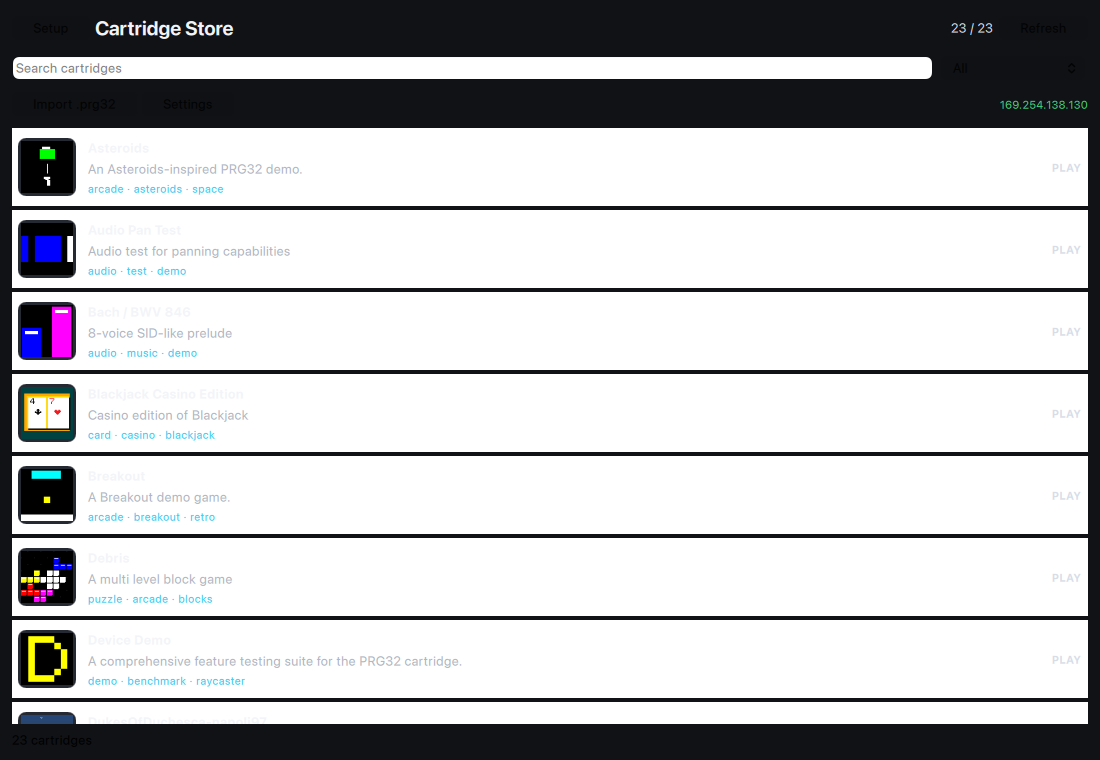
\includegraphics[width=0.78\linewidth]{figures/prg32qt-store.png}
\captionof{figure}{The Cartridge Store browser inside PRG32-QT. Downloads are
architecture-aware: the application asks the Store for a variant it can run
\citep{prg32qt}.}
\label{fig:qtstore}
\end{center}

The controls mirror the kit. On a keyboard the arrow keys (or
\kbtn{W}\,\kbtn{A}\,\kbtn{S}\,\kbtn{D}) are the joystick, \kbtn{Z} or \kbtn{J} is
button~A, \kbtn{X} or \kbtn{K} is button~B, and \kbtn{Enter} or \kbtn{Space} is
Start/Select. A USB or Bluetooth game controller is recognised when it is plugged
in; phones and tablets show touch controls instead.

Students who want to study the host itself can build its Qt-free core, which
contains the cartridge parser, the RV32IMAC interpreter, and the ABI
implementation, and run its test suite without installing Qt at all.

\lstinputlisting[style=bash,
  caption={Building and testing the portable runtime core of PRG32-QT.}
]{scripts/prg32qt/build_core.sh}

\section{Three performance profiles}

An interpreter on a laptop is far faster than a 160\,MHz microcontroller, so a
cartridge that is comfortable in PRG32-QT might crawl on the board. To keep
students honest, the application offers three profiles in its Settings.

\begin{center}
\begin{tabularx}{\linewidth}{@{}lX@{}}
\toprule
Profile & Behaviour \\
\midrule
Accurate (default) & charges each instruction class and each ABI call a
  deterministic cost at the reference 160\,MHz clock and 33\,ms frame cadence;
  reports frames that would have been late on the board \\
Optimal & paces the game at 30 frames per second \\
Unlimited & runs as fast as the host allows \\
\bottomrule
\end{tabularx}
\captionof{table}{PRG32-QT performance profiles \citep{prg32qt}.}
\end{center}

\begin{prgwarn}
Accurate mode is a \emph{model}, not a measurement. It reproduces behaviour that
is visible to a portable cartridge; it is not a cycle-exact simulation of the
ESP32\nobreakdash-C6. Treat its ``late frame'' counter as an early warning, and
confirm any performance claim on real hardware with the method of
Appendix~\ref{app:perf}.
\end{prgwarn}

\section{The debugger: a microscope for the frame loop}

Open Settings, enable \emph{Run cartridges in RISC-V debug mode}, and run a
cartridge. The player stays on the left and remains playable; on the right a
panel shows the disassembled cartridge, the thirty-two integer registers, and a
window onto guest memory.

\begin{center}
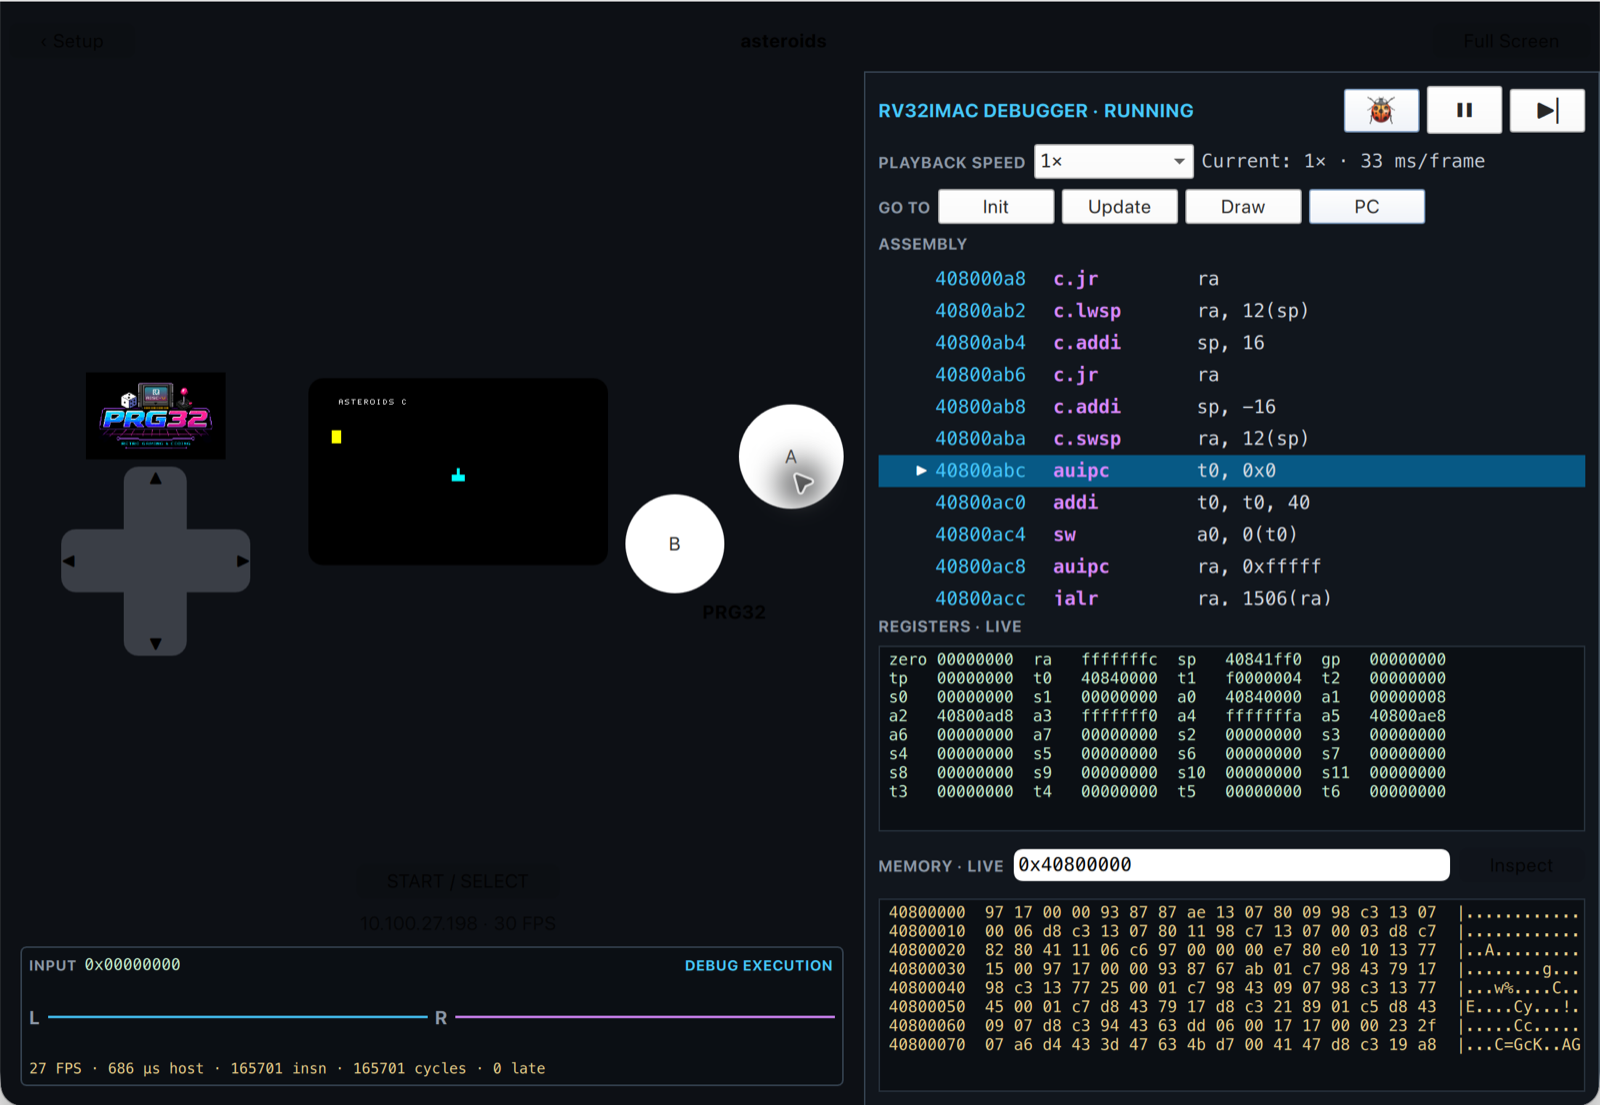
\includegraphics[width=\linewidth]{figures/prg32qt-debugger.png}
\captionof{figure}{The PRG32-QT debugger: the running game, the live assembly
listing with the next instruction highlighted, the registers, and a memory dump
\citep{prg32qt}.}
\label{fig:qtdebugger}
\end{center}

\begin{center}
\begin{tabularx}{\linewidth}{@{}lX@{}}
\toprule
Control & What it does \\
\midrule
Pause / Resume & stop and continue the cartridge; game input is frozen while
  paused \\
Step & execute exactly the highlighted instruction and stay paused \\
Speed & slow motion or fast forward, from $0.01\times$ to $4\times$ \\
Init / Update / Draw & jump the listing to that entry point without executing
  anything \\
PC & follow the live program counter \\
Gutter click & set or clear a breakpoint on that instruction \\
Memory address & show 128 bytes of guest memory in hexadecimal and ASCII \\
\bottomrule
\end{tabularx}
\captionof{table}{The debugger controls.}
\label{tab:qtdebug}
\end{center}

Everything the assembly track asks you to imagine becomes something you can
watch. Chapter~\ref{ch:asm1} says that \code{call} writes the return address into
\reg{ra}; step over a \code{call} and see \reg{ra} change. Chapter~\ref{ch:asm2}
says the input bitmask arrives in \reg{a0}; set a breakpoint after
\code{call prg32\_input\_read}, hold the left arrow, resume, and read
\code{0x00000001} in \reg{a0}. The cartridge is loaded at address
\code{0x40800000}, so a variable declared in \code{.data} can be found by typing
its address into the memory field and watching the bytes change as you play.

\begin{prgtry}
Build the complete C Pong of Appendix~\ref{app:worked} and import it into
PRG32-QT in debug mode. Select \textbf{Update}, set a breakpoint on its first
instruction, and resume. When execution stops, step until you pass the call to
\code{prg32\_input\_read}. Record \reg{a0} three times: with no key held, with
the left arrow held, and with left and \kbtn{Z} held together. Explain the three
values using Table~\ref{tab:buttons}.
\end{prgtry}

\begin{prgaside}
The home computers this book admires shipped with a ``monitor'': a tiny built-in
program that let the owner stop the machine, inspect memory, and change it by
hand. A generation of programmers learned how a processor works by pressing a
freeze button in the middle of a game. A debugger that pauses a running
cartridge and shows its registers is the same idea, forty years on.
\end{prgaside}

\section{Driving PRG32-QT from the toolchain}

While it runs, PRG32-QT announces itself on the local network as
\code{\_prg32.\_tcp.local.} and serves the same small HTTP interface as the
board, so the upload command you already know works against it. It adds one
route the constrained firmware does not have, \code{/api/debug}, and the \prg
tooling wraps that route in a \code{debug} command \citep{prg32repo,prg32qt}.

\lstinputlisting[style=bash,
  caption={Deploying a cartridge to a running PRG32-QT and controlling its
  debugger from a script.}
]{scripts/prg32qt/deploy_and_debug.sh}

This turns the debugger into a laboratory instrument. A script can pause a
cartridge, step a fixed number of instructions, read the registers as JSON, and
compare them with the values a student predicted on paper.

\begin{prgwarn}
The device API is meant for a trusted classroom network. It accepts uploads and
debugger commands from anyone who can reach the port. Do not expose it to the
open Internet.
\end{prgwarn}

\section{Choosing the right target}

A sensible working rhythm uses all three hosts. Develop and debug in PRG32-QT,
where a build takes seconds and a wrong branch can be watched as it is taken.
Confirm in QEMU, which runs the real firmware and therefore the real loader,
status bands, and setup menu. Finish on the board, where time, sound, and the
feel of the joystick are real.

\begin{prgcheck}
You are ready to continue when you can run a Store cartridge in PRG32-QT, import
one you built yourself, pause it, single-step an instruction, and say which
register changed. You should also be able to explain why a frame rate observed
in PRG32-QT is not evidence about the board.
\end{prgcheck}


% Part II --- The Computer Architecture Track (Assembly)
\part{The Computer Architecture Track: RISC-V Assembly}
\chapter{First Contact: Registers, Memory, and the Call}
\label{ch:asm1}

This chapter begins the computer architecture track. By its end you will have a
running \riscv assembly program on both QEMU and, if you have one, the physical
board: a program that clears a console, prints text, and makes a sound. More
importantly, you will understand the three ideas on which everything else rests:
what a register is, how a value lives in memory, and what happens when you call a
function. We build these ideas on the smallest possible game, the ASCII version
of Pong, exactly as the platform's own tutorial does \citep{prg32tutorialascii}.

\section{The machine you are programming}

A \riscv processor of the kind in your board is, from the programmer's point of
view, astonishingly simple. It has thirty-two registers, each holding a 32-bit
value, and it executes instructions that, with few exceptions, do one of three
things: an arithmetic or logical operation between registers, a transfer of a
value between a register and memory, or a change in which instruction runs next.
That is very nearly the whole machine. The richness of computing comes not from a
large instruction set but from combining a small one in long sequences.

\begin{prgconcept}
A register is a tiny, extremely fast storage location inside the processor that
holds one 32-bit value. The processor can only compute on values that are in
registers. To work on a value stored in memory, you must first \emph{load} it
into a register; to keep a result, you must \emph{store} it back to memory.
\end{prgconcept}

The thirty-two registers have conventional roles, fixed not by the hardware but
by an agreement called the \emph{calling convention} or \emph{ABI}. Following the
convention is what lets your assembly code and the framework's C code call each
other. Table~\ref{tab:registers} shows the registers you will actually use; the
full convention is in Appendix~\ref{app:api}.

\begin{center}
\begin{tabularx}{\linewidth}{@{}llX@{}}
\toprule
Register & Name & Role in this book \\
\midrule
\reg{a0}--\reg{a7} & arguments & values passed into and out of calls; \reg{a0} also holds the return value \\
\reg{t0}--\reg{t6} & temporaries & scratch values; a call may destroy them \\
\reg{s0}--\reg{s11} & saved & values a call promises to preserve \\
\reg{ra} & return address & where a \code{ret} jumps back to \\
\reg{sp} & stack pointer & top of the stack; kept 16-byte aligned \\
\reg{zero} & zero & always reads as 0 \\
\bottomrule
\end{tabularx}
\captionof{table}{The \riscv registers you will use, and their agreed roles
\citep{prg32abi}.}
\label{tab:registers}
\end{center}

\begin{prgconcept}
The \textbf{calling convention} is an agreement about which registers carry
arguments (\reg{a0}--\reg{a7}), which carry results (\reg{a0}), and which survive
a function call (\reg{s0}--\reg{s11}, but not \reg{t0}--\reg{t6}). \prg follows the
standard \riscv convention, which is exactly why an assembly game can call a C
helper such as \code{prg32\_gfx\_clear} \citep{prg32tutorial}.
\end{prgconcept}

\section{The smallest program that runs}

Recall the three-function contract from Chapter~\ref{ch:platform}. The smallest
legal \prg game provides \code{init}, \code{update}, and \code{draw} that each do
nothing but return. In \riscv assembly, ``return'' is the instruction \code{ret},
and ``do nothing else'' is simply not writing anything else. We name our game
\code{hello} and give every symbol that prefix.

\lstinputlisting[
    style=asm,
    caption={%
        \fname{hello\_world\_asm.S} \protect\\
        The smallest \prg assembly game: three functions that return immediately.
        Build it, confirm it runs, then add to it.%
    }
]{examples/asm_first_contact/hello_world_asm.S}

A few details deserve explanation. The directive \code{.option norelax} tells the
assembler not to apply an optimisation that can interfere with the way \prg
cartridges are linked; every example begins with it \citep{prg32tutorialgraphic}.
The \code{.section .text} directive says that what follows is executable code, as
opposed to data. The \code{.global} directives make the three symbols visible to
the framework, which must find them by name. Without \code{.global}, your
functions would exist but the loader could not see them.

\begin{prgcheck}
Build this skeleton for QEMU and confirm it runs without crashing. You will see
no game yet: that is correct. The achievement is that the framework found your
three functions, called them, and survived. Chapter~\ref{ch:firstbuild} has the exact
build commands for your operating system; Appendix~\ref{app:worked} shows this
skeleton wired into the firmware.
\end{prgcheck}

\section{Cartridge building and uploading}

The repository contains a quick-start guide in \fname{README.md} and documentation
in the \fname{docs/} folder. For convenience, scripts and tools are provided to
build cartridges, stage them for QEMU, or upload them to a board over Wi\-Fi.

\subsection{ESP32-C6 hardware}

To upload a cartridge to a real board, build it first and then use the included
Python tool. Note that the board IP is \code{192.168.4.1} by default.

\begin{lstlisting}[style=bash,caption={Build and upload a portable cartridge to the board}]
python3 -m prg32 cartridge build examples/games/pong/graphics/game.S \
  --portable --entry-prefix pong_graphics --name pong \
  --architecture esp32c6 --out build-esp32c6/pong.prg32
python3 -m prg32 esp32c6 upload build-esp32c6/pong.prg32 \
  --url http://192.168.4.1
\end{lstlisting}

\subsection{QEMU}

To stage a cartridge for QEMU, build it, inject it into the image, and then
launch the emulator.

\begin{lstlisting}[style=bash,caption={Build and stage a portable cartridge for QEMU}]
python3 -m prg32 cartridge build examples/games/pong/graphics/game.S \
  --portable --entry-prefix pong_graphics --name pong \
  --architecture qemu --out build-qemu/pong.prg32
python3 -m prg32 qemu upload build-qemu/pong.prg32
python3 -m prg32 qemu run
\end{lstlisting}

These commands work on both macOS and Linux. For additional details, see
\fname{README.md} and the files in \fname{docs/} (for example \fname{docs/usage/qemu.md}).

\begin{prgtargets}
\textbf{Both targets.} The cartridge format is identical; what changes is the
architecture label you pass (\code{esp32c6} versus \code{qemu}) and the
delivery (\code{upload} over Wi-Fi versus \code{qemu upload} into the flash
image). Your game source is byte-for-byte the same in both cases
\citep{prg32qemu}.
\end{prgtargets}

\begin{prgwarn}
Always pass \code{--portable}. A portable cartridge reaches the framework through
the numbered ABI table instead of fixed firmware addresses, so it keeps working
when the firmware is rebuilt. Older, firmware-specific cartridges were linked
against one particular firmware image; the current tool refuses to build them.
If a runtime rejects your cartridge, read the message: it names the ABI hash or
the feature it was missing.
\end{prgwarn}

\section{Simple instructions and program structure}

A working program is built from a few very small operations. These
operations are provided by the RISC-V Instruction Set Architecture \citep{riscvisa}.
We will now introduce the foundational operations you need for writing
your first programs.

\subsection{Arithmetic and bit operations}

The first group is the arithmetic and bitwise instructions. In a real program
these are used to update counters, combine values, compute flags, and prepare
arguments for later work. They all read values from registers and write the
result back into a register. The result is stored in the first register.

\begin{center}
\begin{tabularx}{\linewidth}{@{}lXl@{}}
\toprule
Instruction & What it does & Example \\
\midrule
\code{add} & Add two registers & \code{add t0, t1, t2} \\
\code{sub} & Subtract one register from another & \code{sub t0, t1, t2} \\
\code{xor} & Bitwise exclusive-or of two registers & \code{xor t0, t1, t2} \\
\code{or} & Bitwise OR of two registers & \code{or t0, t1, t2} \\
\code{and} & Bitwise AND of two registers & \code{and t0, t1, t2} \\
\bottomrule
\end{tabularx}
\end{center}

The RISC-V ISA also provides immediate forms of many of these operations.
These instructions take one register operand and one small constant, which is
useful for adding a fixed amount or applying a fixed mask in one step.

\begin{center}
\begin{tabularx}{\linewidth}{@{}lXl@{}}
\toprule
Instruction & What it does & Example \\
\midrule
\code{addi} & Add a register and a constant & \code{addi t0, t1, 4} \\
\code{xori} & Exclusive-or a register with a constant & \code{xori t0, t1, 1} \\
\code{ori} & OR a register with a constant & \code{ori t0, t1, 0xff} \\
\code{andi} & AND a register with a constant & \code{andi t0, t1, 7} \\
\bottomrule
\end{tabularx}
\end{center}

\subsection{Load and store word}

A second group of instructions moves whole 32-bit values between memory and
registers. In a real program these are the only instructions that touch the
state stored in the program data; they let the program remember values
from one frame to the next.

\begin{center}
\begin{tabularx}{\linewidth}{@{}lXl@{}}
\toprule
Instruction & What it does & Example \\
\midrule
\code{lw} & Load a 32-bit word from memory into a register & \code{lw t0, 0(t1)} \\
\code{sw} & Store a 32-bit word from a register into memory & \code{sw t0, 0(t1)} \\
\bottomrule
\end{tabularx}
\end{center}

Each load or store combines a register holding a memory address with a small
constant offset. That makes it easy to access fields inside a data structure or
variables laid out in memory. You can use a zero offset when you don't need it.

\subsection{Pseudo-instructions}

The final group is the pseudo-instructions. They are not separate hardware
operations; instead, they are convenient shortcuts that the assembler expands 
into one or more real instructions. In everyday code they make assembly 
easier to read and write.

\begin{center}
\begin{tabularx}{\linewidth}{@{}lXl@{}}
\toprule
Pseudo & What it does & Example \\
\midrule
\code{la} & Load the address of a symbol into a register & \code{la a0, title} \\
\code{li} & Load a constant value into a register & \code{li t0, 42} \\
\code{mv} & Copy one register to another & \code{mv t0, t1} \\
\code{not} & Bitwise complement of a register & \code{not t0, t1} \\
\bottomrule
\end{tabularx}
\end{center}

In practice, \code{la} is used whenever a program needs the address of a string
or a data variable. \code{li} is used to load a number directly into a register
without first storing it in memory. \code{mv} is simply a copy, and \code{not}
computes the one’s complement of a register value.

With these instruction families, the RISC-V ISA provides the basic operations a
program needs: arithmetic and bitwise logic, memory load/store, and the
pseudo-instructions that make assembly manageable. The next section shows how
this instruction set is used when your assembly calls into the framework.

\section{Calling a C helper: the stack frame}
A game that only returns is not interesting for long. The first useful thing we
can do is print text, using the framework's console. The console is written in C,
so calling it means crossing the boundary between your assembly and the
framework's C, and that boundary has one rule a beginner must internalise.

When you execute \code{call}, the processor records, in the register \reg{ra},
the address it should return to. But the C function you are calling will itself
use \reg{ra} for its own calls, overwriting yours. If you do nothing to protect
your \reg{ra}, then when your function tries to \code{ret}, it will jump to the
wrong place and your program will misbehave or crash. The solution is to save
\reg{ra} on the \emph{stack} before the call and restore it afterwards.

\begin{prgconcept}
The \textbf{stack} is a region of memory that grows downward and is used to save
values across function calls. Before calling a C helper, an assembly function
lowers the stack pointer \reg{sp} to make room, stores \reg{ra} there, makes its
call, then loads \reg{ra} back and raises \reg{sp}. This save/restore pair is the
single most important habit in \riscv assembly.
\end{prgconcept}

Here is the pattern, which you will repeat in nearly every function:

\lstinputlisting[
    style=asm,
    caption={%
        \fname{print\_asm.S} \protect\\
        The stack-frame idiom. Save \reg{ra}, do work that may call C, restore \reg{ra}, return.%
    }
]{examples/asm_first_contact/print_asm.S}


Read this slowly, because it contains five distinct ideas. The \code{addi sp, sp,
-16} subtracts sixteen from the stack pointer, reserving sixteen bytes; we use a
multiple of sixteen because the convention requires \reg{sp} to stay 16-byte
aligned across calls \citep{prg32abi}. The \code{sw ra, 12(sp)} stores the word in
\reg{ra} at an offset of twelve bytes above the new stack top. The \code{la a0,
title} loads the \emph{address} of our string into \reg{a0}, because the
convention puts the first argument in \reg{a0} and the console function expects a
pointer. The two \code{call} instructions invoke C helpers. Finally the load and
\code{addi} undo the save and the reservation, in the reverse order, before
\code{ret}.

\begin{prgwarn}
Forgetting \code{sw ra} before a \code{call}, or \code{lw ra} after it, is the
classic first bug. The symptom is a function that ``returns to the wrong place'':
the program jumps somewhere unexpected, often crashing. If your assembly behaves
strangely around a call, check the \reg{ra} save/restore pair first
\citep{prg32tutorialascii}.
\end{prgwarn}

\begin{prgaside}
Why does the stack grow \emph{downward}, toward smaller addresses? It is a
convention almost as old as the stored-program computer, and it lets the stack
and the program's data grow toward each other from opposite ends of memory,
making the most of a fixed address space. Subtracting from \reg{sp} to allocate,
and adding to free, follows directly from that choice.
\end{prgaside}

\section{Assembly sections: the anatomy of a program}

When writing assembly, you must explicitly tell the assembler how to categorize different 
parts of your program using directives. The \code{.section} keyword is the switch that selects 
where the following code or data belongs: \code{.data} for mutable state, \code{.rodata} for constants, 
and \code{.text} for executable instructions. The \code{.data} section is for mutable state—variables 
like our counter that the program must modify during execution. Conversely, \code{.rodata} stands for 
``read-only data'' and is reserved for constants, such as our game title string. On physical hardware, 
placing constants in \code{.rodata} allows the toolchain to keep them safely locked in flash memory so 
they cannot be accidentally overwritten by a bug.

The very first directive in a PRG example is often \code{.option norelax}. That tells the assembler 
not to apply its relaxation pass, so it does not rewrite certain branch or symbol addresses later. 
For PRG32 cartridges, the exact layout of code and data matters, and \code{.option norelax} helps keep 
that layout predictable.

While section directives dictate \emph{where} data lives in memory, the \code{.global} directive 
dictates \emph{who} can see it. By default, every label you define in an assembly file is strictly 
private to that file. By marking a label as \code{.global}, you export it into the project's global 
symbol table. This step is what bridges your assembly code to the rest of the ecosystem, explicitly 
giving the game framework permission to locate, link against, and jump into your functions from the outside.

\section{Values in memory: the \code{.data} section}

A game must remember things between frames: where the ball is, what the score
is. In assembly, persistent values live in the \code{.data} section, each given a
label and an initial value. This is the assembly equivalent of a global variable.
For ASCII Pong, the platform's example declares its state exactly this way
\citep{prg32repo}:

\lstinputlisting[
    style=asm,
    caption={%
        \fname{game\_state\_data.S} \protect\\
        Game state in \code{.data}. Each label names a memory location holding one 32-bit word.%
    }
]{examples/asm_first_contact/game_state_data.S}

To use such a value you do two things, and the distinction between them is the
crux of understanding memory. First you load the \emph{address} of the label into
a register with \code{la}. Then you load the \emph{value} at that address with
\code{lw}, or store a new value with \code{sw}.

\lstinputlisting[
    style=asm,
    caption={%
        \fname{load\_modify\_store.S} \protect\\
        The load--modify--store cycle: read a value from memory, change it in a register, write it back.%
    }
]{examples/asm_first_contact/load_modify_store.S}

\begin{prgconcept}
A label such as \code{hello\_x} names a \emph{location} in memory. \code{la t0,
hello\_x} puts that location's address in \reg{t0}; \code{lw t1, 0(t0)} reads the
\emph{contents} of that location into \reg{t1}. The processor computes only on
contents, in registers, then writes results back. This load--modify--store cycle
is how every variable in every program ultimately works.
\end{prgconcept}

\begin{prgwarn}
Keep the two clearly apart in your mind: \reg{t0} holds an \emph{address}, \reg{t1}
holds a \emph{value}. Confusing them, using an address where a value belongs, or
vice versa, produces wrong numbers and is one of the most common beginner errors.
A useful habit, used throughout the platform's examples, is to comment each
register with whether it holds an address or a value.
\end{prgwarn}

\section{Putting it together: a console game that ticks}

We now have every piece needed for a minimal but genuine program: an \code{init}
that prints a title, an \code{update} that advances a counter each frame, and a
\code{draw} that prints the score to screen.
We also included a short beep sound that works with the \code{prg32\_audio\_beep} call.
\citep{prg32tutorialascii}.

\lstinputlisting[
    style=asm,
    caption={%
        \fname{counter.S} \protect\\
        A counter example that displays an incrementing score.%    
    }
]{examples/asm_first_contact/counter.S}

This short program demonstrates the core design pattern of every game on this platform. 
Notice how the work is split across distinct phases: \code{counter\_update} handles the logic 
by modifying our variable in memory, while \code{counter\_draw} focuses purely on presentation. 
This separation of concerns is fundamental; it ensures that your game mechanics remain entirely 
independent of how or when the screen is drawn.

The program also highlights how data types behave at the machine level through our choice 
of console helpers. While \code{prg32\_console\_write} requires the memory address of a null-terminated 
ASCII string, \code{prg32\_console\_hex32} takes a raw 32-bit numeric value directly in \reg{a0}. It 
reads the content of the register itself and formats that raw integer into human-readable text 
on the fly. Confusing these two---passing a raw number where an address is expected---is a classic 
recipe for a crash.

Finally, look at the entry and exit points of all three functions. Every single one opens 
with an identical prologue to lower \reg{sp} and save \reg{ra}, and closes with a matching 
epilogue to restore them. Because every function here uses a \code{call} instruction to hand 
off work to the framework, they would all overwrite their own return path without this defensive 
housekeeping.

\begin{prgtargets}
\textbf{Both targets.} On QEMU you will see the title on the serial monitor. The
beep uses the legacy buzzer helper: it is audible only on a board that has a
passive buzzer fitted, and silent on QEMU and on the current reference board,
which uses an I2S amplifier instead. Chapter~\ref{ch:asmcap} shows the mixer
call that replaces it and sounds on every host. The
\emph{source is identical}; only the build directory and configuration profile
differ, as shown in Chapter~\ref{ch:platform}.
\end{prgtargets}

\begin{prgtry}
Change the beep frequency from \code{440} to \code{880} and rebuild. On the board,
the tone rises by an octave. Then change the increment in \code{hello\_update}
from \code{1} to \code{2} and predict, before running, what the counter does.
Verify your prediction. This ``change one thing, predict, verify'' loop is the
method of the entire book \citep{prg32repo}.
\end{prgtry}

\begin{prgcheck}
You should now be able to build and run an assembly program on at least QEMU;
explain why \reg{ra} must be saved before a \code{call}; explain the difference
between \code{la} and \code{lw}; and describe what the \code{.data}, \code{.text},
and \code{.rodata} sections are for. If any of these is shaky, re-read the
relevant section before Chapter~\ref{ch:asm2}; everything ahead builds on them.
\end{prgcheck}

\chapter{State and Input: Branches, Bitmasks, and Boundaries}
\label{ch:asm2}

In Chapter~\ref{ch:asm1} a counter advanced on its own. A game, though, responds
to a player. This chapter teaches the assembly you need to read the controller
and to make decisions: the input bitmask, the bitwise \code{andi} test, and the
conditional branch. By the end you will move an object with the joystick and keep
it on the screen: the core interactive loop of every game in this book. We follow
the structure of the platform's ASCII Pong update routine, which was written to be
read by first-year students \citep{prg32tutorialascii,prg32repo}.

\section{Decisions: the conditional branch}

So far our instructions ran in a straight line. To respond to the player, a
program must choose: if a button is pressed, move; otherwise, do not. In \riscv
this choice is a \emph{conditional branch}, an instruction that jumps to a label
only when a condition holds.

\begin{prgconcept}
A \textbf{conditional branch} compares registers and jumps to a label only if the
comparison is true; otherwise execution simply continues to the next instruction.
The branch is how a processor makes every decision, from ``is this button
pressed?'' to ``has the ball hit the wall?''
\end{prgconcept}

The branches you will use most are few. \code{beqz t, label} jumps if \reg{t} is
zero; \code{bltz t, label} jumps if \reg{t} is negative; \code{ble a, b, label}
jumps if \reg{a} $\le$ \reg{b}; and the unconditional \code{j label} always jumps.
A common idiom, which surprises beginners, is to branch on the \emph{opposite} of
what you want: to do something ``if the button is pressed,'' you test the button
bit and \code{beqz}, branch away, when it is \emph{not} pressed, letting the
movement code run only when it is. This reads backwards at first but becomes
natural quickly.

\begin{prgaside}
Local labels written as a bare number followed by a colon, like \code{1:}, and
referenced as \code{1f} (the next \code{1} ``forward'') or \code{1b} (``backward''),
are an assembler convenience for short jumps that need no memorable name. The
platform's examples use them heavily for the small skips inside an update routine
\citep{prg32repo}.
\end{prgaside}

\section{Reading the controller}

Recall from Chapter~\ref{ch:platform} that \prg returns all buttons at once as a
bitmask. In assembly you obtain it by calling \code{prg32\_input\_read}; the
result arrives, by convention, in \reg{a0}. The very first thing to do is copy it
somewhere safe, because the next \code{call} you make would overwrite \reg{a0}.

\lstinputlisting[
    style=asm,
    caption={%
        \fname{get\_input.S} \protect\\
        Read the input bitmask and keep it. The copy to a temporary is essential, because later calls reuse \reg{a0}.%    
    }
]{examples/asm_state_and_input/get_input.S}

\begin{prgwarn}
Copy the input mask out of \reg{a0} immediately. \reg{a0} is the argument and
return register; the moment you call another function, its old contents are gone.
The platform's examples copy the mask into a temporary on the very next line for
exactly this reason \citep{prg32tutorialascii}.
\end{prgwarn}

To test a single button you isolate its bit with \code{andi}, the
``and-immediate'' instruction, using the bit value from
Table~\ref{tab:buttons}. The result is non-zero exactly when that button is
pressed.

\lstinputlisting[
    style=asm,
    caption={%
        \fname{button\_test.S} \protect\\
        Testing one button. \code{andi} keeps only the chosen bit; \code{beqz} skips the body when that bit is clear.%    
    }
]{examples/asm_state_and_input/button_test.S}

\begin{prgconcept}
\code{andi t3, t0, 1} computes the bitwise AND of the input mask with the
constant \code{1}, leaving in \reg{t3} the value of bit~0 alone. If LEFT is
pressed, \reg{t3} is non-zero; if not, it is zero. Testing a button is therefore
``mask the bit, then branch on whether the result is zero.''
\end{prgconcept}

\section{Moving an object with the joystick}

We now assemble a complete \code{update} that moves an object left and right with
the joystick. The state is a single word in \code{.data}, exactly as in
Chapter~\ref{ch:asm1}. The routine reads input, tests LEFT and RIGHT, and updates
the position. For now, we limit the draw to displaying the position on screen.
    In the future, the position will make a graphics object move 
    
    \citep{prg32repo}.

    \lstinputlisting[
        style=asm,
        caption={%
            A full update: read input, move on LEFT/RIGHT, store the result. 
            Compare with the platform's \texttt{pong\_ascii\_update}.%
        }
    ]{examples/asm_state_and_input/input_read.S}

Trace it once by hand. Suppose \code{game\_x} holds \code{20} and the player
holds RIGHT. The input read returns a mask with bit~1 set. The LEFT test
(\code{andi ... 1}) yields zero, so \code{beqz} skips the left move. The RIGHT
test (\code{andi ... 2}) yields non-zero, so the right move runs and \reg{t2}
becomes \code{21}. The store writes \code{21} back. Next frame it becomes
\code{22}, and so on. The object slides right as long as RIGHT is held. This kind
of by-hand trace is the most valuable debugging skill you will build in this
course.

The code also introduces a tiny performance trick. Instead of redrawing the
screen on every update, it stores a small flag in \code{text\_update} whenever
LEFT or RIGHT actually changes \code{game\_x}. The draw routine checks this
flag and skips the clear/write sequence when nothing moved. In the previous
chapter, the example redrew continuously, but a real game should avoid doing
work when the state does not change.

There is also something to notice about the numbers on screen. If you move
left past zero, the value underflows and the display shows \code{0xffffffff} instead
of a normal count. If you move right past \code{9}, the console printer keeps
counting in hexadecimal, so \code{10} appears as \code{a}, \code{11} as
\code{b}, and so on. That is because we are displaying the 
32 bit score word is displayed as an hexadecimal value.

\section{Staying on the screen: the boundary clamp}

Left unchecked, our object will slide right off the edge of the screen and
vanish. The fix is a \emph{clamp}: after computing the new position, force it back
into the legal range. For the 40-column ASCII console the legal range is 0 to 39;
for the 320-pixel graphics viewport it will be 0 to a value that accounts for the
object's width. The logic is identical either way.

\lstinputlisting[
    style=asm,
    caption={%
        \fname{x\_clamping.S} \protect\\
        Clamping x to the range [0, 39]. Negative values snap to 0; values past the edge snap to the maximum.% %
    }
]{examples/asm_state_and_input/x_clamping.S}

\begin{prgconcept}
A \textbf{boundary clamp} keeps a value inside a legal range: if it went below the
minimum, set it to the minimum; if above the maximum, set it to the maximum;
otherwise leave it alone. Almost every off-screen bug in a beginner's game is a
missing or wrong clamp. When an object disappears, suspect the clamp first.
\end{prgconcept}

\begin{prgwarn}
The maximum is not the screen width; it is the screen width minus the object's
own size. A 64-pixel-wide paddle on a 320-pixel screen may go no further right
than $320-64 = 256$, or its right edge would leave the viewport. The platform's
graphics Pong clamps the paddle to exactly \code{256} for this reason
\citep{prg32repo}.
\end{prgwarn}

\begin{prgtry}
Add the clamp above to your \code{update}. Write
one sentence explaining which comparison protects the right edge. This
break-and-fix exercise is taken directly from the platform's labs
\citep{prg32tutorialgraphic}.
\end{prgtry}

\section{Debugging like a systems programmer}

When an assembly game misbehaves, the platform's guidance is explicit and worth
adopting as a discipline: do not guess, trace state \citep{prg32tutorial}. Ask, in
order, which register held the last correct value, which instruction changed it,
whether a \code{call} overwrote a temporary you expected to keep, and whether a
branch skipped the code that updates memory. Reduce the program to the smallest
version that still shows the bug. Nine times in ten the answer is one of three
things: a missing \reg{ra} save, an address-versus-value confusion, or a branch
that goes the wrong way.

\begin{prgcheck}
You should now be able to read the input bitmask into a register; test an
individual button with \code{andi} and \code{beqz}; move a value in \code{.data}
in response to the joystick; and clamp that value to a legal range. With these,
you have written the interactive core of a game. Chapter~\ref{ch:asm3} adds the
one missing ingredient: drawing it on the screen.
\end{prgcheck}

\chapter{Drawing the Game: Graphics, Collision, and the Frame}
\label{ch:asm3}

You can now move an object with the joystick and keep it on the screen. This
chapter gives that object a body. We move from the text console to the
320-by-200 graphics viewport, draw rectangles for a paddle and a ball, detect
when they touch, and tie the three functions together into a complete, playable
graphical Pong game. \citep{prg32qemu,prg32tutorialgraphic}.

\section{A blank frame}

We start with a \code{draw} that clears the screen to black and does nothing else: confirm it runs.

\lstinputlisting[
    style=asm,
    caption={%
        \fname{hello\_world\_graphics.S} \protect\\
       A \code{draw} that clears the frame. Build this first and confirm%
       a black screen before drawing anything on it.%
    }
]{examples/asm_graphics_game/hello_world_graphics.S}

\section{Drawing a rectangle}

The mental model from ASCII based programs is unchanged: state lives in \code{.data},
\code{update} changes it, \code{draw} renders it. What changes is the drawing
call. Instead of \code{prg32\_console\_write}, we use \code{prg32\_gfx\_clear} to
erase the frame and \code{prg32\_gfx\_rect} to draw a filled rectangle.

To draw a rectangle, we use the call \code{prg32\_gfx\_rect(x, y, w, h, color)}. 
In assembly the five arguments go, in order, into \reg{a0} through \reg{a4}, 
following the calling convention. The colour in \reg{a4} is an RGB565 value; 
you may write it as a named constant in C,
but in assembly it is usually a plain number: \code{65535} for white,
\code{65504} for yellow, \code{0} for black \citep{prg32repo}.

\begin{prgwarn}
The five arguments of \code{prg32\_gfx\_rect} occupy \reg{a0}=x, \reg{a1}=y,
\reg{a2}=width, \reg{a3}=height, \reg{a4}=colour. Getting an argument into the
wrong register draws the wrong rectangle: a vivid, immediate way to see what the
calling convention actually means.
\end{prgwarn}

In the next full example we will draw a white paddle near the bottom of the viewport,  
at a position read from \code{.data}. The other dimensions are constant: we will draw
a 64-by-8 white bar at $y=188$. Wide enough to be easy to see in the emulator and
perfect for recreating the old classic Pong. \citep{prg32repo}. Here is what
the paddle draw section will look like:

\lstinputlisting[
    style=asm,
    caption={%
        \fname{paddle\_draw.S} \protect\\
       Drawing the paddle from a stored position. The five arguments fill \reg{a0}--\reg{a4} in order.%
    }
]{examples/asm_graphics_game/paddle_draw.S}

\section{The ball: position, velocity, and the bounce}

Now we need a ball. The ball needs four words of state: its $x$ and $y$ position
and its $x$ and $y$ velocity (which the examples call \code{dx} and \code{dy}).
Each frame, the velocity is added to the position; when the ball reaches an edge,
the velocity is negated so it travels back the other way. \citep{prg32repo}.

\lstinputlisting[
    style=asm,
    caption={%
        \fname{ball\_motion.S} \protect\\
       Autonomous ball motion on the x and y axis with edge bounce.%
    }
]{examples/asm_graphics_game/ball_motion.S}

\begin{prgconcept}
\textbf{Velocity} is just a number added to position each frame. A \emph{bounce}
is negating that number when the object reaches a boundary: \code{neg t4, t4}
turns $+2$ into $-2$, so the next frames move the ball back the way it came. With
this one idea: add velocity and negate at the edges, you can make anything bounce.
\end{prgconcept}

\section{Did they touch? Rectangle collision}

A ball that passes straight through the paddle is no fun. We need to know when
the ball's rectangle overlaps the paddle's rectangle. The framework provides
exactly this test: \code{prg32\_sprite\_hitbox(ax, ay, aw, ah, bx, by, bw, bh)}
takes the position and size of two rectangles and returns non-zero when they
overlap \citep{prg32tutorialgraphic}. In assembly the eight arguments fill
\reg{a0} through \reg{a7}.

\lstinputlisting[
    style=asm,
    caption={%
        \fname{collision\_detection.S} \protect\\
       Testing ball-versus-paddle overlap. A non-zero result in \reg{a0} means they touched this frame.%
    }
]{examples/asm_graphics_game/collision_detection.S}

Two rectangles overlap when they intersect on \emph{both} axes at once: the $x$
ranges overlap \emph{and} the $y$ ranges overlap. \code{prg32\_sprite\_hitbox}
performs this two-axis test for you and returns the answer as a single value, so
collision becomes one call followed by one branch.

\begin{prgconcept}
Notice that the bounce reuses the clamp from Chapter~\ref{ch:asm2}, with one
addition: where the clamp merely stopped the object at the edge, the bounce also
negates the velocity. The platform's examples keep the clamp so the ball never
visibly leaves the screen even for a single frame, then negate so it returns. Good
game feel often comes from such small combinations of simple rules.
\end{prgconcept}

\section{Assembling the complete game}

We now have every part: a paddle moved by input and clamped, a ball that moves
and bounces, and a collision test. Putting them in the three functions gives a
complete graphical game whose structure exactly matches the platform's
\code{pong\_graphics} example \citep{prg32repo}. The \code{update} moves the 
paddle from input,  advances and bounces the ball, and applies collision; 
the \code{draw} clears the frame and renders the paddle and ball.

\lstinputlisting[
    style=asm,
    caption={%
        \fname{pong\_skeleton.S} \protect\\
       The \code{draw} of the complete game. Compare it line for line%
        with \code{pong\_graphics\_draw} in the repository.%
    }
]{examples/asm_graphics_game/pong_skeleton.S}

A brief stylistic note: earlier chapters tended to use simple numeric 
labels for branch targets; in this chapter we switch to descriptive, 
named labels for different sections of control flow. This is a readability 
improvement only; it does not change program behaviour but makes the 
structure and intent of each labelled section easier to follow.

\begin{prgtargets}
\textbf{Both targets.} Develop and watch this on the QEMU virtual screen, 
where the ball bounces and the paddle responds to injected input. Then 
build the identical source for the ESP32\nobreakdash-C6 to play it with 
a real joystick and hear the beep. Because QEMU's defaults disable the 
physical GPIO buttons, the paddle may sit still in the emulator unless 
input is injected; the ball still moves, so the render path is fully 
verified on the desktop \citep{prg32qemu}.
\end{prgtargets}

\section{Step-by-step: how this game was built}

It is worth making explicit the pedagogical order in which a game like this is
constructed, because it is the order the platform recommends and the order in
which the example games in \code{examples/games} were themselves written
\citep{prg32tutorial,prg32tutorialgraphic}.

First, write \code{init}, \code{update}, and \code{draw} that only return, 
and confirm the framework runs them. Second, add one \code{.data} variable.
Third, read input in \code{update} and move the objects, then add clamping. 
Fourth, add the collision test. Only then, fifth, add sound on the collision 
event. Each step is buildable and observable on its own; if a step breaks, 
the bug is in the few lines you just added, not hidden in a wall of untested code.

\begin{prgtry}
Build the game incrementally in exactly these five steps, rebuilding and running
after each. Keep a short log: after each step, write one line saying what you
added and what you saw. This log is not busywork: it is the written form of the
``change one thing, observe, record'' method, and it will make the difference
between a frustrating afternoon and a productive one \citep{prg32repo}.
\end{prgtry}

\begin{prgcheck}
You can now clear the frame, draw rectangles from stored state, move the ball
with velocity and bounces, and detect collisions with one call. You have, in
other words, built a complete graphical game in \riscv assembly that runs on both
targets. Chapter~\ref{ch:asmcap} turns this into a capstone you extend and
package as a cartridge.
\end{prgcheck}

\chapter{Capstone: Extending and Shipping an Assembly Game}
\label{ch:asmcap}

A program that runs only when embedded in the firmware is a lab exercise; a
program packaged as a cartridge is a game you can hand to someone. This closing
chapter of the assembly track does two things. First, it extends the Pong of
Chapter~\ref{ch:asm3} into a fuller game by reading, not rewriting, the
platform's richer examples. Second, it ships your work: it builds your source
into a \fname{.prg32} cartridge and deploys it to both QEMU and the physical
board without reflashing the firmware \citep{prg32tutorial,prg32cartfmt}.

\section{Reading is a skill: Breakout as Pong with bricks}

You will spend far more of your career reading code than writing it, and the
platform's example games are designed to be read. Once you have written Pong, the
Breakout example is legible at a glance: it is Pong with an extra piece of
state, a row of bricks, and one extra rule: removing a brick when the ball hits
it \citep{prg32repo}. The Breakout source even stores its bricks as a small bitmask,
the same bitmask idea you learned for the input in Chapter~\ref{ch:asm2}, now
repurposed so that each set bit means ``this brick is still present.''

\begin{prgconcept}
A bitmask is not only for input. Breakout packs a row of bricks into the bits of a
single word: bit $i$ set means brick $i$ is intact, clear means it has been
knocked out. Testing a brick is \code{andi}; clearing one is a bitwise AND with
the complement of its bit. The same instruction you used to read a button now
manages a row of bricks.
\end{prgconcept}

\begin{prgtry}
Open \fname{examples/games/breakout/graphics/game.S} and find the line that
declares the brick state (it is a single \code{.word} near the top, holding a
small mask). Then find, in \code{update}, where a brick is removed. Write two
sentences: one naming the register that holds the brick mask, and one explaining
which bitwise operation clears a brick. You are now reading assembly the way a
maintainer does \citep{prg32repo}.
\end{prgtry}

\section{Extending your own game}

Before packaging, extend the Pong you built in Chapter~\ref{ch:asm3} with one new
feature of your choosing. The platform's suggested progression, one moving
object, one collision, one score counter, then sound, means the natural next
features are a score that increases on a successful bounce, a second collision
surface, or a beep on the event \citep{prg32tutorial}. Add exactly one, build it,
and confirm it on QEMU. Resist the urge to add three features at once; the whole
method of this book is that a single change is easy to verify and a triple change
is not.

A score is the gentlest extension and reinforces the load--modify--store cycle
from Chapter~\ref{ch:asm1}. In \code{update}, when the collision test succeeds,
read the score word, add one, and store it back. In \code{draw}, render it with
\code{prg32\_gfx\_text8}, whose arguments are the position, the string, and a
foreground and background colour. Because turning a number into a string is
fiddly in pure assembly, a good first version simply draws a fixed label such as
\code{"SCORE"} and proves the text path works; printing the digits can come later
with the console's \code{prg32\_console\_hex32} helper, which displays a value in
hexadecimal without any string conversion on your part \citep{prg32repo}.

\begin{prgwarn}
Increment the score on the \emph{event}, not every frame. The collision test is
true for as long as the rectangles overlap, which may be several frames, so a
naive ``add one whenever overlapping'' counts a single hit many times. The robust
pattern is to act on the \emph{transition} into overlap; a simple version remembers
whether the ball was overlapping last frame and scores only when it newly
overlaps. This is the same ``act on the event'' discipline as the beep warning in
Chapter~\ref{ch:platform}.
\end{prgwarn}

\section{Sound that works everywhere: the mixer call}

The beeps in the earlier chapters used the legacy buzzer helper. The call below
uses the runtime's mixer, which sounds on the board's amplifier, on QEMU, and in
PRG32-QT alike. It also shows a pattern worth learning for its own sake:
detecting the \emph{edge} of a button, the frame in which it goes from released
to pressed, by comparing this frame's bitmask with the previous one.

\lstinputlisting[style=asm,
  caption={\fname{examples/asm\_capstone/audio\_note\_event.S}: one note per new
  press of A. Five arguments, in \reg{a0}--\reg{a4}.}
]{examples/asm_capstone/audio_note_event.S}

\begin{prgtry}
Run this cartridge in the PRG32-QT debugger (Chapter~\ref{ch:qt}). Put a
breakpoint on the \code{beqz}. Hold A and resume twice. Explain, from the values
of \reg{s0} and \reg{t1}, why the note plays on the first stop and not on the
second.
\end{prgtry}

\section{Building a cartridge}

When your firmware has been flashed once and your game source is ready, the
command \code{python3 -m prg32 cartridge build} compiles and packages it into a
\fname{.prg32} cartridge. The tool needs your source file, the \code{--portable}
flag, the entry-point prefix that names your three functions, a human-readable
name, and an output path \citep{prg32tutorial}. It no longer needs the firmware
itself: a portable cartridge calls the framework through the ABI table.

\begin{lstlisting}[style=bash,caption={Building, inspecting, and running your assembly game.}]
python3 -m prg32 cartridge build work/mygame/game.S \
  --portable --entry-prefix mygame --name mygame \
  --out work/mygame/mygame.prg32
python3 -m prg32 cartridge summary work/mygame/mygame.prg32
python3 -m prg32 qemu upload work/mygame/mygame.prg32
python3 -m prg32 qemu run
\end{lstlisting}

The \code{summary} command prints what the firmware will read: the ABI version
and hash, the import model, the code and memory sizes, and the feature bits. It
is the quickest way to confirm that a cartridge is what you think it is.

\begin{prgconcept}
A cartridge bundles your three compiled functions with a small header that the
firmware reads to find them. The \code{--entry-prefix} you pass is how the tool
knows which symbols are your \code{init}, \code{update}, and \code{draw}; it must
exactly match the prefix in your \code{.global} directives. A mismatch here is a
common build-time error, and the message names the symbol it could not find.
\end{prgconcept}

\section{When it goes wrong}

The platform ships a self-check command that verifies your toolchain
prerequisites and the partition layout before you spend time chasing an error
\citep{prg32repo}. If a cartridge upload to QEMU fails, the usual cause is a
missing or invalid QEMU flash image file; run QEMU once to create it, then stage
again. If the board shows a black screen, the usual cause is targeting the
wrong firmware variant, as warned in Chapter~\ref{ch:platform}. These are not
exotic failures; they are the everyday friction of embedded work, and learning
to read the error and apply the known fix is itself part of the curriculum.

\begin{prgcheck}
The assembly track is complete. You can read a register-level game written by
someone else; you can extend a game by one well-tested feature; and you can
package your work as a cartridge and deploy it to both the emulator and real
hardware. You have, end to end, written and shipped a native \riscv program.
Appendix~\ref{app:worked} contains the full annotated source of the games
referenced here, and Appendix~\ref{app:api} is your reference for every framework
call you have used.
\end{prgcheck}


% Part III --- The Computer Programming Track (C)
\part{The Computer Programming Track: The C Language}
\chapter{First Contact: Functions, Variables, and the Game Loop in C}
\label{ch:c1}

This chapter begins the computer programming track. It is independent of the
assembly track: you need not have read Part~II, only the shared foundation in
Part~I. Here you will write a complete retro game in C, running on both QEMU and
the ESP32\nobreakdash-C6. The same three-function shape from Chapter~\ref{ch:platform}
organises the work, but where assembly exposed registers and the stack, C lets you
write the game's logic almost as plainly as you would describe it in words
\citep{prg32tutorialc}.

\section{Why C, and why the same platform}

C occupies a deliberate middle ground. It is a high-level language, you write
functions, name variables, and use \code{if} and \code{while}, yet it stays close
enough to the machine that nothing important is hidden. A C variable is a named
box in memory; a C function compiles to the very calling convention you would
write by hand in assembly. By learning C on the same platform, the same display,
and the same two targets used for the architecture course, you keep your attention
on the language and the game logic rather than on a new toolchain
\citep{prg32teaching}. If you later read Part~IV, you will see your C compiled into exactly the same assembly idioms used in Part~II.

\begin{prgconcept}
The platform runs C and assembly games through the identical \code{init},
\code{update}, \code{draw} contract and the identical framework interface. The
only thing that changes between the two tracks is the language you express the
logic in. This is why the platform can serve both a computer architecture course
and a computer programming course from one codebase \citep{prg32teaching}.
\end{prgconcept}

\section{The three functions, in C}

In C, the three entry points are ordinary functions returning \code{void}, named
with your game's prefix. The framework calls \code{<prefix>\_init} once and then
\code{<prefix>\_update} and \code{<prefix>\_draw} once per frame, exactly as in the
assembly track \citep{prg32tutorialc}. To use the framework, include one header.

\lstinputlisting[
    style=c,
    caption={%
        \fname{hello\_world\_c.c}: The smallest C game. Three functions that do nothing yet: the C counterpart of the assembly skeleton in Chapter~\ref{ch:asm1}.%
    }]{examples/c_first_contact/hello_world_c.c}

The single \code{\#include "prg32.h"} gives you every framework function and every
named constant: the button bits, the colours, and the screen dimensions that you
met in Chapter~\ref{ch:platform}. You never declare these yourself; the header does
it for you. For a complete list, you can check Appendix~\ref{app:api}.

\begin{prgcheck}
Build this skeleton for QEMU and confirm it runs without crashing and shows a
blank screen. As in the assembly track, an empty screen is the correct first
result: the framework has found and called your three functions.
\end{prgcheck}

\section{State: variables that persist between frames}

A game remembers things between frames. In assembly that meant the \code{.data}
section; in C it means variables declared outside the functions, at file scope,
so they keep their values from one frame to the next. The platform's C Pong
declares its paddle and ball state exactly this way \citep{prg32repo}.

\lstinputlisting[
    style=c,
    caption={%
        \fname{pong\_c\_state.c} \protect\\
       Game state as file-scope variables. Declared outside the functions, they persist across frames. \texttt{static} keeps them private to this file.}
]{examples/c_first_contact/pong_c_state.c}

The \code{init} function is where you can set the starting values of the variables.
In the pong example, this is where the initial position and velocities are set.

\lstinputlisting[
    style=c,
    caption={%
        \fname{pong\_c\_init.c} \protect\\
       Initialising state in \code{init}. This runs once, before the first frame.}
]{examples/c_first_contact/pong_c_init.c}

\begin{prgconcept}
File-scope variables in C play the role that labelled words in \code{.data} play
in assembly: they are the game's persistent state. \code{init} gives them their
opening values; \code{update} changes them each frame; \code{draw} reads them to
render. Keeping state in named variables, rather than recomputing it, is what
makes a game a game rather than a static picture.
\end{prgconcept}

\section{Reading input: the bitmask in C}

Input works just as it did in Chapter~\ref{ch:platform}: one call returns a
bitmask, and you test a button with bitwise AND against a named constant. In C the
call returns a value you store in a variable, and the test is an \code{if}.

\lstinputlisting[
    style=c,
    caption={%
        \fname{pong\_c\_update.c} \protect\\
       Reading input and moving the paddle. Note the bitwise \texttt{\&}, not \texttt{==}, exactly as warned in Chapter~\ref{ch:platform}.}
]{examples/c_first_contact/pong_c_update.c}

\begin{prgwarn}
Use \code{input \& PRG32\_BTN\_LEFT}, with a single ampersand for bitwise AND, not
\code{input == PRG32\_BTN\_LEFT}. The mask may hold several buttons at once; the
bitwise test asks ``is the left bit set, regardless of the others,'' which is what
you want. This is the same warning as in the assembly track, and it catches
beginners in both languages \citep{prg32tutorialc}.
\end{prgwarn}

The two clamps at the end are the boundary check from Chapter~\ref{ch:asm2},
written in C. The maximum is the screen width minus the paddle's own width, so the
paddle's right edge never leaves the viewport. In C the clamp is two short
\code{if} statements; the logic is identical to the assembly version, only more
compact.

\section{The ball: velocity and bounce, in C}

The ball moves by adding its velocity to its position each frame and bounces by
negating its velocity at the edges: the same rule as in
Chapter~\ref{ch:asm3}, now in three lines of C \citep{prg32repo}.

\lstinputlisting[
    style=c,
    caption={%
        \fname{pong\_c\_ball\_motion.c} \protect\\
        Ball motion and edge bounce. Adding velocity moves the ball; negating it at the boundary turns it around.}
]{examples/c_first_contact/pong_c_ball_motion.c}

\section{Collision: one call, one decision}

To bounce the ball off the paddle, ask the framework whether their rectangles
overlap. \code{prg32\_sprite\_hitbox} takes the position and size of two
rectangles and returns non-zero when they touch, so collision is a single call
inside an \code{if} \citep{prg32repo}.

\lstinputlisting[
    style=c,
    caption={%
        \fname{pong\_c\_paddle\_collision.c} \protect\\
        Bouncing the ball off the paddle. The hitbox test returns non-zero on overlap.}
]{examples/c_first_contact/pong_c_paddle_collision.c}

\begin{prgconcept}
Collision detection in C is one function call and one \code{if}. The framework
does the geometric work of testing overlap on both axes; you decide what happens
when the answer is yes. This separation, the engine answers ``did they touch,''
your code decides ``so what'', is a pattern you will meet throughout game
programming.
\end{prgconcept}

\section{Drawing the frame}

The \code{draw} function clears the viewport and renders each object as a coloured
rectangle, using the named colour constants from the header. The \code{draw} function 
reads the state variables but does not change them; all logic stays in \code{update}.
We do this to follow the phase separation from Chapter~\ref{ch:platform}.
\citep{prg32tutorialc}.

\lstinputlisting[
    style=c,
    caption={%
        \fname{pong\_c\_draw.c} \protect\\
        Rendering the frame. \code{draw} only reads state and puts pixels; it changes nothing.}
]{examples/c_first_contact/pong_c_draw.c}

Now we can look at the full Pong example, built in C. If you followed the assembly course,
you can compare it line by line with the previous version.

\lstinputlisting[
    style=c,
    caption={%
        \fname{pong\_skeleton.c} \protect\\
        Rendering the frame. \code{draw} only reads state and puts pixels; it changes nothing.}
]{examples/c_first_contact/pong_skeleton.c}

\begin{prgtargets}
\textbf{Both targets.} This complete C Pong runs unchanged on QEMU and the
ESP32\nobreakdash-C6. On the emulator you watch the ball bounce and verify the layout; on
the board you play it with a real joystick.
\end{prgtargets}

\begin{prgtry}
Change the paddle colour from \code{PRG32\_COLOR\_WHITE} to
\code{PRG32\_COLOR\_CYAN} and the ball size from \code{8} to \code{12}, then
rebuild. Both changes should be visible immediately. Next, the platform's
break-and-fix exercise: delete the \code{paddle\_x > 256} clamp, rebuild, hold
RIGHT until the paddle leaves the screen, then restore the clamp and explain in one
sentence which condition protects the boundary \citep{prg32tutorialc}.
\end{prgtry}

\begin{prgcheck}
You can now write a complete C game: persistent state in file-scope variables,
input read as a bitmask and tested with \code{\&}, motion by velocity with
boundary clamps, bounce by negation, collision by one call, and rendering kept
separate in \code{draw}. Chapter~\ref{ch:c2} scales these ideas up with the C
features, arrays and structs, that let a game hold many objects and a whole
world.
\end{prgcheck}

\chapter{A Bigger World: Arrays, Structs, and Tile Maps}
\label{ch:c2}

The Pong of Chapter~\ref{ch:c1} held a handful of separate variables. Real games
hold many things at once: rows of bricks, swarms of enemies, a whole landscape of
ground and platforms. This chapter introduces the two C features that make such
games manageable: the \emph{array}, which holds many values of the same kind, and
the \emph{struct}, which groups related values into one named thing, and applies
them to a tile-based platform game built on the platform's own example
\citep{prg32repo,prg32tutorialc}.

\section{Arrays: many values under one name}

An array is a numbered row of values of the same type. Where Pong needed one
paddle position, Breakout needs a position, or simply a present/absent flag, for
each of many bricks, and writing a separate variable for each would be absurd. An
array lets you store them together and reach any one by its index.

\lstinputlisting[
    style=c,
    caption={%\fname{brick\_flags.c} \protect\
       An array of brick flags. Index $i$ holds whether brick $i$ is still present.}
]{examples/c_structs_and_tiles/brick_flags.c}

\begin{prgconcept}
An array stores many values of one type in a numbered sequence; \code{bricks[i]}
is the value at index \code{i}, counting from zero. A \code{for} loop visits every
element in turn. Together, the array and the loop replace dozens of separate
variables and the repetitive code that would manage them.
\end{prgconcept}

The framework itself uses small arrays to describe artwork. An 8-by-8 tile: a
patch of ground, a coin or a hazard, is stored as an array of eight bytes, one per
row, where each bit is a pixel. The platformer example defines its tiles exactly
this way \citep{prg32repo}.

\lstinputlisting[
    style=c,
    caption={%
        \fname{coin\_tile.c} \protect\\
         An 8-by-8 tile as an array of eight bytes. Each byte is one row; each bit is one pixel. This is the platformer's coin tile.}
]{examples/c_structs_and_tiles/coin_tile.c}

\begin{prgaside}
Reading the bits of \code{tile\_coin} as ones and zeros, top to bottom, sketches a
small round coin: the rows are narrow at top and bottom and wide in the middle.
Defining graphics as bit patterns in arrays is exactly how the home computers of
the retro era stored their character sets and sprites, with artists working in
hexadecimal on grid paper. The technique is old, compact, and still perfectly
legible.
\end{prgaside}

\section{Structs: grouping what belongs together}

A moving character has several attributes that always travel together: its
position, its velocity, its size, its state. Keeping them in separate arrays that
must be kept in step is error-prone. A \emph{struct} bundles them into a single
named value, so the whole character is one thing you can pass around. The framework
defines such a struct for platform-game characters, \code{prg32\_platform\_actor\_t}.
This is used in the platformer example, which can be found in \fname{examples/games/platformer/c/game.c}
\citep{prg32repo}.

\lstinputlisting[
    style=c,
    caption={%\fname{platform\_actor\_struct.c} \protect\
       The framework's actor struct (from \texttt{prg32.h}). Position, velocity, size, and state, grouped into one value.}
]{examples/c_structs_and_tiles/platform_actor_struct.c}

\begin{prgconcept}
A struct groups related values into one named type. With
\code{prg32\_platform\_actor\_t player;} you create a single \code{player} whose
position is \code{player.x}, velocity \code{player.vx}, and so on. Passing one
struct is cleaner and safer than passing six loose variables, and it scales: an
array of structs is a crowd of characters.
\end{prgconcept}

\section{A tile map: the world as a grid}

A platform game's world is too large to draw as individual rectangles. Instead it
is a \emph{tile map}: a grid in which each cell names a tile to draw there. The
framework provides a two-layer playfield for this, and you fill it by placing tile
identifiers at grid coordinates with \code{prg32\_playfield\_put} \citep{prg32repo}.
The platformer example builds its landscape with small helpers that draw runs and
columns of tiles: ordinary loops over the grid.

\lstinputlisting[
    style=c,
    caption={%\fname{put\_run.c} \protect\
       Filling a run of ground tiles with a loop. The platformer uses helpers like this to lay out its world.}
]{examples/c_structs_and_tiles/put_run.c}

\begin{prgconcept}
A tile map represents a large world compactly: instead of remembering every pixel,
it remembers, for each grid cell, which small reusable tile belongs there. Drawing
the world becomes drawing the grid; building the world becomes filling the grid
with loops. This is how side-scrolling games fit sprawling levels into tiny
memory.
\end{prgconcept}

\section{Behaviour from tile flags}

A tile is not only a picture; it can carry \emph{behaviour}. The framework lets you
attach flags to a tile identifier, solid, platform, hazard, collectable, and then
the physics helpers know how a character should interact with it. You declare, for
instance, that tile~2 is solid, and from then on a character cannot walk through
it \citep{prg32repo}.

\lstinputlisting[
    style=c,
    caption={%\fname{tile\_flags.c} \protect\
       Giving tiles behaviour. Marking a tile solid makes the physics helper treat it as ground or wall.}
]{examples/c_structs_and_tiles/tile_flags.c}

\section{Putting it together: an actor in a world}

With an actor struct, a tile map, and tile flags, a platform game's per-frame
logic becomes remarkably short. The framework's \code{prg32\_platform\_actor\_step}
reads the input, applies gravity, moves the actor, and resolves collisions against
the solid tiles, updating the struct's \code{state} flags so your code can react
to what happened \citep{prg32repo,prg32tutorialc}.

\lstinputlisting[
    style=c,
    caption={%\fname{platform\_physics.c} \protect\
       One frame of platform physics. The helper does the movement and collision; your code reads the resulting state.}
]{examples/c_structs_and_tiles/platform_physics.c}

A single call advances the whole character: the joystick moves
it, gravity pulls it down, the solid tiles stop it, and the returned \code{state}
tells you if it touched a hazard. The camera-follow call then scrolls the tile map
so the character stays in view. The same behaviour written from first principles
would be a page of code; the struct and the helper compress it because they capture
exactly the data and the operation the problem needs.

\begin{prgwarn}
Pass the \emph{address} of the actor, \code{\&player}, to the stepping and
follow helpers, not the struct by value. These functions must \emph{change} the
actor, its position and state, and in C a function can only change a value the
caller can see if it is given that value's address. Forgetting the \code{\&} is a
common error; the symptom is an actor that never moves, because the function
updated a private copy.
\end{prgwarn}

\begin{prgtry}
Open \fname{examples/games/platformer/c/game.c} and find where it defines the coin
tile and where it marks a tile collectable. Add one new platform to the world by
calling \code{put\_run} with new coordinates, rebuild for QEMU, and confirm your
platform appears. Then change the \code{gravity} argument of
\code{prg32\_platform\_actor\_step} from \code{1} to \code{2} and describe how the
jump feels different. One change, observed and recorded \citep{prg32repo}.
\end{prgtry}

\begin{prgcheck}
You can now hold many values in arrays, group related values in structs, represent
a world as a tile map filled by loops, and give tiles behaviour with flags. These
are the data-structuring ideas a programming course exists to teach, learned here
on a game you can see and play. Chapter~\ref{ch:ccap} brings them together into a
capstone you extend and ship as a cartridge.
\end{prgcheck}

\chapter{Capstone: Extending and Shipping a C Game}
\label{ch:ccap}

This chapter closes the C track the way Chapter~\ref{ch:asmcap} closed the
assembly track: by extending a game and shipping it. You will embed a C game in
the firmware for quick iteration, build it into a \fname{.prg32} cartridge, and
deploy it to both QEMU and the board. Along the way you will meet two ideas that
recur in serious systems programming: reusing helper functions, and doing
arithmetic without a floating-point unit, both grounded in the platform's richer
C examples \citep{prg32tutorialc,prg32repo}.

\section{Embedding a C game in the firmware}

For fast iteration during development, the platform lets you compile a C game
directly into the firmware instead of packaging a cartridge each time. You add the
game's source to the firmware's build list and call its three functions from the
main loop \citep{prg32tutorialc}. This is a temporary lab arrangement, restored
afterwards, but it shortens the edit-build-run cycle while you are still changing
the game often.

\lstinputlisting[
    style=c,
    caption={%\fname{pong\_c\_firmware\_loop.c} \protect\
       Calling a C game's three functions from the firmware's main loop. \texttt{init} once, then \texttt{update} and \texttt{draw} each frame, with a present and a short delay.}
]{examples/c_capstone/pong_c_firmware_loop.c}

\begin{prgconcept}
The frame loop you met as a diagram in Chapter~\ref{ch:platform} is, in the
firmware, a literal \code{while (1)} that calls \code{update}, then \code{draw},
then \code{prg32\_gfx\_present} to display the frame, then waits briefly so the
game runs at a steady rate. Embedding your game here lets you see the loop you have
been writing the body of all along.
\end{prgconcept}

\begin{prgwarn}
The embedding is temporary. The platform's tutorial is explicit that you should
restore the firmware's default main loop and build list after the lab, so the
resident firmware returns to loading cartridges normally \citep{prg32tutorialc}.
Keep a clean copy, or use version control (Appendix~\ref{app:github}) so restoring
is one command.
\end{prgwarn}

\section{Reusing helpers and reading richer examples}

Once your game grows, repeated code is a liability. C's answer is the helper
function: a named, reusable piece of logic you write once and call many times. You
already saw the platformer's \code{put\_run} and \code{put\_column} helpers in
Chapter~\ref{ch:c2}; they exist precisely so the world-building code is not a wall
of near-identical lines. When you extend your own game, watch for three or more
lines that recur with small variations, and lift them into a helper.

The platform's raycaster example is the next step for a class ready for more
\citep{prg32teaching}. It renders a Doom-style corridor, a convincing pseudo-3-D
view, on the same \riscv runtime used for everything else. What makes it
instructive is not the 3-D effect but \emph{how} it computes that effect without a
floating-point unit.

\section{Arithmetic without floating point: fixed point}

Small microcontrollers often have no hardware for fractional numbers, yet a
raycaster needs fractions: half a step, a third of an angle. The classic solution,
used by the platform's raycaster, is \emph{fixed-point arithmetic}: represent a
fractional value as an integer that has been scaled up by a fixed factor, do the
arithmetic in integers, then scale back down \citep{prg32tutorialc,prg32repo}.

\lstinputlisting[
    style=c,
    caption={%\fname{raycast\_fixed\_point.c} \protect\
       Fixed-point in the raycaster. Direction vectors are stored scaled by 256; multiplying and then dividing by 256 keeps the fraction.}
]{examples/c_capstone/raycast_fixed_point.c}

\begin{prgconcept}
\textbf{Fixed-point arithmetic} stores a fractional number as an integer scaled by
a fixed factor: here, 256. A value of $1.5$ is stored as $384$, because
$1.5\times256=384$. Multiplications are done in integers and then divided by the
scale to bring the result back. This lets a processor with no floating-point unit
compute smooth motion and angles using only integer instructions, a technique as
old as real-time graphics and still used in embedded systems today.
\end{prgconcept}

\begin{prgaside}
The notation ``Q8'' in the example names the format: eight bits of fraction, so a
scale of $2^8 = 256$. Fixed-point was the only practical way to do fast fractional
maths on the home computers of the retro era, and the raycaster's corridor is a
direct descendant of the techniques that made early 3-D games run on machines with
no floating-point hardware at all. Learning it here is learning a genuine piece of
computing history that remains useful.
\end{prgaside}

\section{Sound, chance, and a scoreboard}

Three small runtime services turn a demonstration into a game people replay.

\emph{Sound.} The mixer call \code{prg32\_audio\_note} plays a MIDI note on one
of eight channels and returns at once. The listing below plays it on the
\emph{edge} of a button press, computed by masking this frame's input with the
complement of the previous frame's.

\lstinputlisting[style=c,
  caption={\fname{examples/c\_capstone/audio\_note\_event.c}: one note per new
  press of A.}
]{examples/c_capstone/audio_note_event.c}

\emph{Chance and scores.} \code{prg32\_random\_number(min, max)} returns a
uniformly distributed value in an inclusive range. The score calls store a
result under the player name saved in the setup menu, show the local
leaderboard, and, when the board is connected to a Cartridge Store, send the
score there too (Chapter~\ref{ch:store}).

\lstinputlisting[style=c,
  caption={\fname{examples/c\_capstone/score\_and\_random.c}: a random spawn and
  a persistent score.}
]{examples/c_capstone/score_and_random.c}

\begin{prgwarn}
A cartridge is a freestanding program: there is no C standard library behind it.
\code{printf}, \code{malloc}, and \code{rand} are not available. Use the helpers
in \fname{prg32.h}, and write the few small utilities you need, such as the
number-to-digits function in the Lemon Catcher of Appendix~\ref{app:worked},
yourself.
\end{prgwarn}

\section{Building and shipping a C cartridge}

The command is the one the assembly track uses; the builder recognises the
\fname{.c} extension and compiles the file as a small freestanding module.

\begin{lstlisting}[style=bash,caption={Building, inspecting, and running a C cartridge.}]
python3 -m prg32 cartridge build work/mygame/game.c \
  --portable --entry-prefix mygame --name mygame \
  --out work/mygame/mygame.prg32
python3 -m prg32 cartridge summary work/mygame/mygame.prg32
python3 -m prg32 qemu upload work/mygame/mygame.prg32   # emulator
python3 -m prg32 esp32c6 upload work/mygame/mygame.prg32 \
  --url http://192.168.4.1                               # board
\end{lstlisting}

Chapter~\ref{ch:firstbuild} has the environment details, and
Chapter~\ref{ch:store} takes the finished file to the Cartridge Store.

\begin{prgtargets}
\textbf{Both targets.} A C cartridge and an assembly cartridge are the same kind of
file and run through the same loader; the framework neither knows nor cares which
language produced the three functions inside \citep{prg32teaching}. This is the
deepest demonstration of the platform's design: several courses, several
languages (the Construction Kit of Part~IV generates C from blocks), one
runtime, one cartridge format.
\end{prgtargets}

\begin{prgtry}
Take the C Pong you wrote in Chapter~\ref{ch:c1}, add a score that increments when
the ball bounces off the paddle, guarding against counting one hit many times, as
warned in Chapter~\ref{ch:asmcap}, and display it with \code{prg32\_gfx\_text8}.
Build it as a cartridge for QEMU and run it. Then, if you have a board, upload the
same cartridge over Wi-Fi and play it. You will have written, extended, packaged,
and shipped a complete C game on real \riscv hardware \citep{prg32repo}.
\end{prgtry}

\begin{prgcheck}
The C track is complete. You can embed a game for fast iteration, factor repeated
logic into helpers, reason about fixed-point arithmetic, and build and deploy a C
cartridge to both targets. With both tracks behind you (or your own track behind
you), Chapter~\ref{ch:join} offers a short, illuminating reunion: the same game,
in both languages, side by side.
\end{prgcheck}


% Part IV --- The Young Makers Track (Blocks, ages 7+)
\part{The Young Makers Track: Blocks with the Construction Kit}
\chapter{Mission 1: Your First Blocks}
\label{ch:kids1}

\begin{prgteacher}
Part~IV is written for children from about seven years old, working with a
teacher, parent, or older student. The sentences are short on purpose, and the
child is addressed directly. Read the chapter aloud with younger pupils; let
older ones read it themselves. Everything an adult needs, from installation to
lesson plans and assessment, is in Chapter~\ref{ch:kitteach}. No hardware is
required: the whole track runs in a web browser.
\end{prgteacher}

Hello, maker! In this part of the book \textbf{you} are going to build video
games. Real ones. You will not type long lines of strange words. You will snap
coloured \emph{blocks} together, like building bricks, and the computer will do
what your blocks say.

\section{What is a program?}

A computer is very fast, but it is not clever. It cannot guess what you want. It
only follows instructions, one after another, exactly as they are written.

A list of instructions for a computer is called a \textbf{program}. A person who
writes programs is called a \textbf{programmer}. Today, that is you.

\begin{prgtry}
Play \emph{Robot} with a friend. You are the programmer; your friend is the
robot. The robot may only do what you say: ``one step forward'', ``turn left'',
``pick up the pencil''. Can you get your robot from the door to the window? What
happens if you forget one instruction?
\end{prgtry}

\section{Meet the Construction Kit}

The tool you will use is called the \textbf{PRG32 Construction Kit}
\citep{prg32kit}. It opens in a web browser, like a web page. Your teacher will
give you the address.

\begin{center}
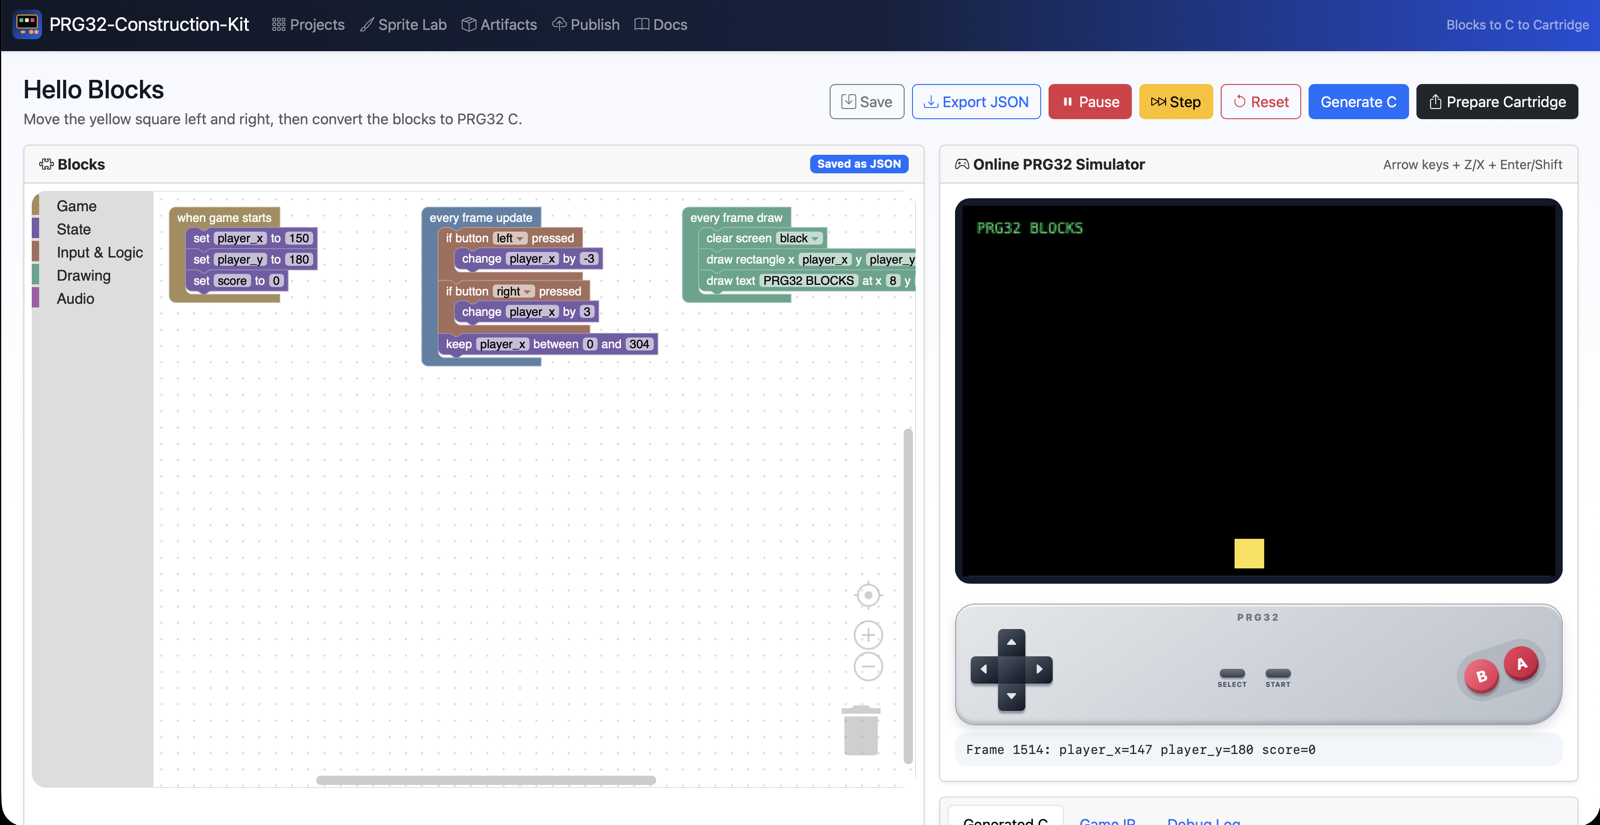
\includegraphics[width=\linewidth]{figures/construction-kit-editor.png}
\captionof{figure}{The Construction Kit. On the left are the blocks. On the
right is the game screen, with a game pad under it \citep{prg32kit}.}
\label{fig:kiteditor}
\end{center}

Look for these four places on the screen:

\begin{itemize}
  \item the \textbf{toolbox}, where the blocks live, sorted by colour;
  \item the \textbf{workspace}, the big empty area where you build;
  \item the \textbf{game screen}, where your game appears;
  \item the \textbf{buttons} at the top: \kbtn{Save}, \kbtn{Play}, \kbtn{Step},
        and \kbtn{Reset}.
\end{itemize}

\begin{prgmission}[Mission 1, step 1: a new project]
\begin{enumerate}
  \item Click \kbtn{New Project}.
  \item Type the title \textbf{First Square}.
  \item Click \kbtn{Create}.
\end{enumerate}
\end{prgmission}

\section{The screen is a grid}

The game screen is made of tiny squares called \textbf{pixels}. There are 320
pixels from left to right and 200 pixels from top to bottom.

To tell the computer \emph{where} to draw, you give it two numbers:

\begin{itemize}
  \item \textbf{x} says how far to the \emph{right};
  \item \textbf{y} says how far \emph{down}.
\end{itemize}

\begin{center}
\begin{tikzpicture}[font=\sffamily\small,scale=0.9]
  \draw[draw=prgink!60,fill=prgink!6,thick] (0,0) rectangle (8,5);
  \fill[prgred] (0,5) circle (2pt) node[above right,text=prgred]{x = 0, y = 0};
  \draw[-{Stealth[length=2.5mm]},thick,prgaccent] (0.4,4.6) -- (3.2,4.6)
    node[right]{x gets bigger};
  \draw[-{Stealth[length=2.5mm]},thick,prgviolet] (0.4,4.6) -- (0.4,2.2)
    node[below right]{y gets bigger};
  \fill[prgamber] (5.3,2.3) rectangle (5.7,2.7);
  \node[below] at (5.5,2.25){x = 152, y = 92};
  \node[anchor=south east] at (8,0.05){x = 319, y = 199};
\end{tikzpicture}
\captionof{figure}{The game screen. The corner at the top left is the
starting point. Going right makes x bigger. Going \emph{down} makes y bigger.}
\label{fig:kidgrid}
\end{center}

\begin{prgwarn}
On a game screen, a \emph{bigger} y is \emph{lower} down. That feels upside
down at first. If something goes down when you wanted up, check your y.
\end{prgwarn}

\section{Three big blocks}

Every game you make has three big yellow blocks. They are in the \textbf{Game}
drawer of the toolbox.

\kgame{when game starts}
\kgame{every frame update}
\kgame{every frame draw}

\begin{itemize}
  \item \textbf{when game starts} runs \emph{one time}, at the beginning. Here
        you get things ready.
  \item \textbf{every frame update} runs again and again, many times each
        second. Here you \emph{change} things.
  \item \textbf{every frame draw} also runs again and again. Here you
        \emph{paint} the picture.
\end{itemize}

A \textbf{frame} is one picture. A cartoon is many pictures shown very quickly,
one after another. A game is the same: get ready once, then change, paint,
change, paint, change, paint\dots

\begin{prgconcept}
A game is a loop. First it gets ready. Then it repeats two jobs forever:
\emph{update} (change the numbers) and \emph{draw} (paint the picture).
\end{prgconcept}

\section{Boxes with names: variables}

A game must remember things: where the player is, how many points you have. It
keeps each thing in a \textbf{variable}. A variable is a box with a name on it
and one number inside.

\begin{center}
\begin{tikzpicture}[font=\sffamily\small]
  \foreach \x/\name/\val in {0/player\_x/152,3.4/player\_y/92}{
    \draw[thick,draw=prgviolet,fill=prgviolet!10,rounded corners=2pt] (\x,0) rectangle ++(2.6,1.4);
    \node[font=\sffamily\bfseries\Large] at (\x+1.3,0.7){\val};
    \node[above,text=prgviolet] at (\x+1.3,1.4){\name};
  }
\end{tikzpicture}
\captionof{figure}{Two variables. Each is a named box with a number inside.}
\end{center}

The purple block \textbf{set} puts a number in a box.

\begin{prgmission}[Mission 1, step 2: get ready]
Drag \textbf{when game starts} into the workspace. Open the purple
\textbf{State} drawer and snap two \textbf{set} blocks inside it. Change the
words and numbers so it looks like this:

\kgame{when game starts}
\kstate[6mm]{set player\_x to 152}
\kstate[6mm]{set player\_y to 92}
\end{prgmission}

\section{Paint the picture}

Now tell the computer what to paint. The green-blue blocks in the
\textbf{Drawing} drawer do that.

\begin{prgmission}[Mission 1, step 3: draw]
Drag \textbf{every frame draw} into the workspace and fill it like this:

\kgame{every frame draw}
\kdraw[6mm]{clear screen BLACK}
\kdraw[6mm]{draw rectangle x player\_x y player\_y w 16 h 16 color YELLOW}
\kdraw[6mm]{draw text HELLO PRG32 at x 8 y 8 fg GREEN bg BLACK}

In the rectangle block, \textbf{w} is how wide and \textbf{h} is how high.
\end{prgmission}

Why \textbf{clear screen} first? Because the computer paints on top of the old
picture. If you do not clean the screen, the old drawings stay.

\begin{prgmission}[Mission 1, step 4: play!]
Click \kbtn{Save}. Then click \kbtn{Play}.

You should see a yellow square in the middle of a black screen, and green words
at the top. You made that!
\end{prgmission}

\section{Change one thing}

Real programmers learn by changing \emph{one} thing and watching what happens.
Try these. After each change, press \kbtn{Reset} and \kbtn{Play}.

\begin{prgtry}
\begin{enumerate}
  \item Change \textbf{player\_x} to 0. Where did the square go?
  \item Change \textbf{player\_x} to 304. Where is it now?
  \item Change \textbf{player\_y} to 184. Is the square higher or lower?
  \item Make the square 64 wide and 8 high. What shape is it?
  \item Change the colour. Change the words.
  \item Add a second rectangle with a different colour. Can you draw a house?
\end{enumerate}
\end{prgtry}

\begin{prgwarn}
The order of blocks matters. Put \textbf{clear screen} \emph{under} your
rectangle and press Play. The square is gone! The computer painted the square,
then painted black over it.
\end{prgwarn}

\section{When something goes wrong}

Mistakes in a program are called \textbf{bugs}. Everybody makes them. Finding
and fixing a bug is called \textbf{debugging}, and it is part of the fun.

\begin{itemize}
  \item \textbf{Nothing on the screen?} Did you press \kbtn{Play}? Is your
        rectangle inside \emph{every frame draw}?
  \item \textbf{Square in the wrong place?} Read your x and y numbers aloud.
  \item \textbf{A block will not snap in?} Blocks only fit inside one of the
        three big yellow blocks.
\end{itemize}

\begin{prgcheck}
You finished Mission~1 if you can:
\begin{itemize}
  \item say what a program is;
  \item point to the top-left corner and say its x and y;
  \item name the three big blocks and say when each one runs;
  \item say what a variable is;
  \item move your square by changing a number.
\end{itemize}
\end{prgcheck}

\begin{prggrownup}
The finished project is in the book's repository as
\fname{examples/blocks\_first\_steps/first\_square.blocks.json}; use
\kbtn{Import JSON} on the Kit's home page to load it. The ``Robot'' game is an
unplugged activity in the tradition of \citet{bell2009}; it is worth ten minutes
before any screen is switched on.
\end{prggrownup}

\chapter{Mission 2 and 3: Move It, Catch It}
\label{ch:kids2}

Your square sits still. A game where nothing moves is not much of a game. In
this chapter you make the square obey the buttons, and then you build a whole
game called \textbf{Lemon Catcher}.

\section{The game pad}

Under the game screen there is a game pad. It has a cross with four arrows, two
round buttons called \kbtn{A} and \kbtn{B}, and two small buttons called
\kbtn{SELECT} and \kbtn{START}. You can click them with the mouse or touch them
with a finger. The arrow keys on the keyboard work too, with \kbtn{Z} for A and
\kbtn{X} for B.

\section{If}

The red block in the \textbf{Input \& Logic} drawer asks a question:

\kinput{if button LEFT pressed}

The blocks you put \emph{inside} it run only when the answer is yes. If the
button is not pressed, the computer skips them.

\begin{prgconcept}
\textbf{If} lets a program choose. \emph{If} the button is pressed, do this.
Otherwise, do nothing and carry on.
\end{prgconcept}

\section{Change}

The purple block \textbf{change} adds a number to a variable.

\kstate{change player\_x by 3}

If player\_x was 152, it becomes 155. Next frame, 158. Then 161. The square
slides to the right.

To go left, x must get \emph{smaller}. So we add a number below zero:

\kstate{change player\_x by -3}

\begin{prgmission}[Mission 2, step 1: move left and right]
Open your First Square project. Drag \textbf{every frame update} into the
workspace and build this:

\kgame{every frame update}
\kinput[6mm]{if button LEFT pressed}
\kstate[12mm]{change player\_x by -3}
\kinput[6mm]{if button RIGHT pressed}
\kstate[12mm]{change player\_x by 3}

Press \kbtn{Save} and \kbtn{Play}. Use the arrows!
\end{prgmission}

\begin{prgtry}
\begin{enumerate}
  \item Change 3 to 1. Then to 10. What does this number do?
  \item Add two more \textbf{if} blocks for UP and DOWN. They must change
        \textbf{player\_y}. Which one needs the minus sign?
\end{enumerate}
\end{prgtry}

\section{Do not fall off the world}

Hold the right arrow for a long time. The square walks off the screen and never
comes back! The variable keeps growing: 320, 330, 340\dots

The purple block \textbf{keep} is a fence. It stops a number from going too low
or too high.

\kstate{keep player\_x between 0 and 304}

Why 304 and not 320? The square is 16 wide. Its left side is at x. If x is 304,
its right side is at $304 + 16 = 320$, exactly the edge.

\begin{prgmission}[Mission 2, step 2: the fence]
Add two \textbf{keep} blocks at the bottom of \emph{every frame update}:

\kstate[6mm]{keep player\_x between 0 and 304}
\kstate[6mm]{keep player\_y between 0 and 184}

Play again. Can the square escape now?
\end{prgmission}

\section{Watching the numbers}

Under the game pad there is a grey line. It shows your variables and their
numbers while the game runs.

Press \kbtn{Play} once more to pause. Now press \kbtn{Step}. The game moves
forward by \emph{one} frame only. Hold the right arrow on the game pad and press
\kbtn{Step} again and again. Watch player\_x: 152, 155, 158\dots

\begin{prgconcept}
\textbf{Step} runs one frame and stops. It lets you slow the computer down
until you can see exactly what your blocks do.
\end{prgconcept}

\section{Mission 3: Lemon Catcher}

Time for a real game. Lemons fall from the sky. You move a basket to catch
them. A green bar grows when you catch one. A red bar grows when you miss.

Start a \textbf{new project} called \textbf{Lemon Catcher}.

\subsection*{The boxes we need}

\begin{center}
\begin{tabular}{@{}ll@{}}
\toprule
Variable & What it remembers \\
\midrule
basket\_x & where the basket is, left to right \\
lemon\_x & where the lemon is, left to right \\
lemon\_y & how far the lemon has fallen \\
score & how many lemons you caught \\
misses & how many lemons you missed \\
\bottomrule
\end{tabular}
\end{center}

\begin{prgmission}[Mission 3, step 1: get ready]
\kgame{when game starts}
\kstate[6mm]{set basket\_x to 144}
\kstate[6mm]{set lemon\_x to 150}
\kstate[6mm]{set lemon\_y to 0}
\kstate[6mm]{set score to 0}
\kstate[6mm]{set misses to 0}
\end{prgmission}

\begin{prgmission}[Mission 3, step 2: draw everything]
\kgame{every frame draw}
\kdraw[6mm]{clear screen BLACK}
\kdraw[6mm]{draw rectangle x lemon\_x y lemon\_y w 10 h 10 color YELLOW}
\kdraw[6mm]{draw rectangle x basket\_x y 180 w 32 h 8 color ORANGE}
\kdraw[6mm]{draw rectangle x 0 y 196 w 320 h 4 color BLUE}

Press \kbtn{Play}. You see a lemon at the top, a basket, and a blue floor.
Nothing moves yet. That is fine. We add one thing at a time.
\end{prgmission}

\begin{prgmission}[Mission 3, step 3: move the basket, drop the lemon]
\kgame{every frame update}
\kinput[6mm]{if button LEFT pressed}
\kstate[12mm]{change basket\_x by -4}
\kinput[6mm]{if button RIGHT pressed}
\kstate[12mm]{change basket\_x by 4}
\kstate[6mm]{keep basket\_x between 0 and 288}
\kstate[6mm]{change lemon\_y by 2}

Play. The basket moves. The lemon falls\dots and falls through the floor.
\end{prgmission}

\section{Touching}

How does the game know the lemon is in the basket? With the other red block:

\kinput{if rect \dots{} touches rect \dots}

``Rect'' is short for \emph{rectangle}. The block has eight numbers: x, y, w
and h for the first rectangle, then x, y, w and h for the second. If the two
rectangles overlap, even a little, the blocks inside run.

\begin{center}
\begin{tikzpicture}[font=\sffamily\small]
  \draw[fill=prgamber!70,draw=prgamber!60!black] (0,0.4) rectangle (0.8,1.2);
  \draw[fill=prgred!50,draw=prgred] (1.6,0) rectangle (4.0,0.5);
  \node at (2,-0.5){not touching};
  \draw[fill=prgred!50,draw=prgred] (6.6,0) rectangle (9.0,0.5);
  \draw[fill=prgamber!70,draw=prgamber!60!black] (7.2,0.3) rectangle (8.0,1.1);
  \node at (7.8,-0.5){touching!};
\end{tikzpicture}
\captionof{figure}{Two rectangles touch when they overlap.}
\end{center}

When you catch a lemon, three things should happen: you get a point, and a new
lemon appears at the top, somewhere new. For ``somewhere new'' there is a
purple block that rolls a dice:

\kstate{set lemon\_x to random from 0 to 310}

\begin{prgmission}[Mission 3, step 4: catch!]
Add this at the bottom of \emph{every frame update}. Type the eight values
carefully: the lemon first, then the basket.

\kinput[6mm]{if rect lemon\_x lemon\_y 10 10 touches rect basket\_x 180 32 8}
\kstate[12mm]{change score by 1}
\kstate[12mm]{set lemon\_y to 0}
\kstate[12mm]{set lemon\_x to random from 0 to 310}
\end{prgmission}

\begin{prgmission}[Mission 3, step 5: miss!]
The blue floor is a rectangle too. If the lemon touches the floor, you missed.

\kinput[6mm]{if rect lemon\_x lemon\_y 10 10 touches rect 0 196 320 4}
\kstate[12mm]{change misses by 1}
\kstate[12mm]{set lemon\_y to 0}
\kstate[12mm]{set lemon\_x to random from 0 to 310}
\end{prgmission}

\section{Showing the score}

The player cannot see inside your variables. Let us draw the score as a bar
that grows. The trick: a width does not have to be a plain number. It can be a
little sum.

\begin{prgmission}[Mission 3, step 6: score bars]
Add these to \emph{every frame draw}, after \textbf{clear screen}:

\kdraw[6mm]{draw text LEMONS at x 8 y 4 fg GREEN bg BLACK}
\kdraw[6mm]{draw rectangle x 64 y 4 w score * 3 h 8 color GREEN}
\kdraw[6mm]{draw text MISSED at x 8 y 16 fg RED bg BLACK}
\kdraw[6mm]{draw rectangle x 64 y 16 w misses * 3 h 8 color RED}

The star \textbf{*} means ``times''. With 5 lemons the bar is $5 \times 3 = 15$
pixels wide. Play, and watch the bars race!
\end{prgmission}

\begin{prgtry}
Make the game your own.
\begin{enumerate}
  \item Make the lemon fall faster. Which number is it?
  \item Make the basket smaller. You must change it in \emph{two} places. Why?
  \item Add a second fruit with its own variables: orange\_x and orange\_y.
  \item Make a ``bad'' fruit that takes away a point when you catch it.
\end{enumerate}
\end{prgtry}

\begin{prgwarn}
If your basket catches nothing, check the \textbf{touches} block. The numbers
there must be the same as the numbers in your \textbf{draw rectangle} blocks.
The computer does not look at the picture. It only looks at the numbers.
\end{prgwarn}

\begin{prgcheck}
You finished Missions~2 and~3 if you can:
\begin{itemize}
  \item explain what \textbf{if} does;
  \item make something move with a button;
  \item say why the fence stops at 304 and not at 320;
  \item use \kbtn{Step} to watch a variable change;
  \item explain how the game knows a lemon was caught.
\end{itemize}
\end{prgcheck}

\begin{prggrownup}
Reference projects: \fname{moving\_square.blocks.json} and
\fname{lemon\_catcher.blocks.json} in \fname{examples/blocks\_first\_steps}.
The Blocks language deliberately has no general comparison block; the ``floor
is a rectangle'' idea in step~5 is how a threshold test is expressed with the
collision block. A complete, playable C rewrite with a numeric score and a
game-over state is in Appendix~\ref{app:worked}, for older siblings and for the
C track.
\end{prggrownup}

\chapter{Mission 4 and 5: Sound, Pictures, and Sharing}
\label{ch:kids3}

Your game works. Now make it \emph{feel} good: add sound, draw your own
pictures, and then put your game on a cartridge so that other people can play
it.

\section{Beep!}

The pink blocks in the \textbf{Audio} drawer make sound.

\kaudio{play beep freq 880 ms 80}

This block has two numbers.

\begin{itemize}
  \item \textbf{freq} is how \emph{high} the sound is. A big number is a high,
        squeaky sound. A small number is a low, growly sound.
  \item \textbf{ms} is how \emph{long} the sound lasts. 1000 is one second, so
        80 is very short.
\end{itemize}

\begin{prgmission}[Mission 4, step 1: happy beep, sad beep]
Open Lemon Catcher. Put a high beep inside the ``caught'' block and a low beep
inside the ``missed'' block:

\kinput{if rect lemon\_x lemon\_y 10 10 touches rect basket\_x 180 32 8}
\kstate[6mm]{change score by 1}
\kaudio[6mm]{play beep freq 880 ms 80}

\kinput{if rect lemon\_x lemon\_y 10 10 touches rect 0 196 320 4}
\kstate[6mm]{change misses by 1}
\kaudio[6mm]{play beep freq 220 ms 150}

Play with the sound on. Can you tell a catch from a miss with your eyes closed?
\end{prgmission}

\begin{prgwarn}
Put sound blocks \emph{inside an if}, so they play only when something
happens. A beep block sitting alone in \emph{every frame update} starts a new
beep every frame, and that is just noise.
\end{prgwarn}

\section{Notes}

The second pink block plays a musical note.

\kaudio{play MIDI note 60 on channel 0 for 250 ms}

Notes have numbers. Note 60 is the \emph{C} in the middle of a piano. Each step
up is the next key.

\begin{center}
\begin{tabular}{@{}lcccccccc@{}}
\toprule
Note name & C & D & E & F & G & A & B & C \\
Number & 60 & 62 & 64 & 65 & 67 & 69 & 71 & 72 \\
\bottomrule
\end{tabular}
\captionof{table}{The white keys from middle C up to the next C.}
\end{center}

\begin{prgmission}[Mission 4, step 2: the Music Pad]
Make a new project called \textbf{Music Pad}. Four buttons play four notes,
and a white bar shows which pad is playing.

\kgame{when game starts}
\kstate[6mm]{set marker\_x to 400}

\kgame{every frame update}
\kstate[6mm]{set marker\_x to 400}
\kinput[6mm]{if button LEFT pressed}
\kstate[12mm]{set marker\_x to 40}
\kaudio[12mm]{play MIDI note 60 on channel 0 for 120 ms}
\kinput[6mm]{if button UP pressed}
\kstate[12mm]{set marker\_x to 104}
\kaudio[12mm]{play MIDI note 64 on channel 0 for 120 ms}

Add two more: RIGHT plays note 67 with the marker at 168, and A plays note 72
with the marker at 232.

\kgame{every frame draw}
\kdraw[6mm]{clear screen BLACK}
\kdraw[6mm]{draw rectangle x 40 y 80 w 48 h 48 color BLUE}
\kdraw[6mm]{draw rectangle x 104 y 80 w 48 h 48 color GREEN}
\kdraw[6mm]{draw rectangle x 168 y 80 w 48 h 48 color RED}
\kdraw[6mm]{draw rectangle x 232 y 80 w 48 h 48 color MAGENTA}
\kdraw[6mm]{draw rectangle x marker\_x y 136 w 48 h 6 color WHITE}
\end{prgmission}

Why is marker\_x set to 400 at the start of every update? The screen is only
320 wide, so 400 is \emph{off the screen}. The bar is hidden there until a
button moves it under a pad. Hiding things off the screen is an old game
maker's trick.

\begin{prgtry}
Play \emph{C, E, G, C}: left, up, right, A. That is a chord called C major.
Change the note numbers to make your own four-note tune. Can a friend copy it
by ear?
\end{prgtry}

\section{Sprite Lab: draw your own pictures}

A small picture used in a game is called a \textbf{sprite}. Click
\textbf{Sprite Lab} at the top of the Kit.

\begin{prgmission}[Mission 4, step 3: a lemon with a face]
\begin{enumerate}
  \item Click \kbtn{New Sprite}. Name it \textbf{lemon}. Keep 16 by 16.
  \item Pick yellow and paint a round lemon, one pixel at a time.
  \item Pick black and give it two eyes and a smile.
  \item Made a mistake? Use the eraser. Erased pixels are see-through.
  \item Click \kbtn{Save}.
\end{enumerate}
\end{prgmission}

A 16 by 16 sprite has $16 \times 16 = 256$ pixels. Every pixel is one colour.
Up close you see squares. From far away you see a lemon. All pictures on all
screens work like this.

\section{What is under the blocks?}

Here is a secret. The computer does not really understand blocks. It
understands a language of words and symbols. One such language is called
\textbf{C}. Grown-up programmers type it by hand.

Click \kbtn{Generate C}. On the right you can see your game written in C.

\begin{center}
\begin{tabularx}{\linewidth}{@{}XX@{}}
\toprule
Your block & The same thing in C \\
\midrule
set score to 0 & \code{score = 0;} \\
change basket\_x by 4 & \code{basket\_x += 4;} \\
if button LEFT pressed & \code{if (input \& PRG32\_BTN\_LEFT) \{ \}} \\
clear screen BLACK & \code{prg32\_gfx\_clear(PRG32\_COLOR\_BLACK);} \\
\bottomrule
\end{tabularx}
\captionof{table}{Each block becomes one line of C.}
\end{center}

\begin{prgtry}
Find the line in the C that came from your \textbf{keep basket\_x between}
block. How many \textbf{if}s did one block turn into?
\end{prgtry}

You do not have to understand all of it. Just notice: your blocks \emph{are} a
real program. One day you may write the words yourself. The older students who
use this book do exactly that.

\section{Mission 5: your game on a cartridge}

Long ago, video games came on \textbf{cartridges}: plastic boxes you pushed
into the machine. \prg games come on cartridges too, but ours are files. A \prg
cartridge file ends in \fname{.prg32}.

\begin{prgmission}[Mission 5, step 1: make the cartridge]
Open your best game. Click \kbtn{Compile Cartridge}.

If your teacher has set up the cartridge tools, green download buttons appear.
You have made a real cartridge!
\end{prgmission}

\begin{center}
\begin{tikzpicture}[font=\sffamily\small,node distance=7mm,
  s/.style={rounded corners=3pt,draw=prgsteel,fill=prgpanel,minimum height=11mm,minimum width=23mm,align=center},
  ar/.style={-{Stealth[length=2.2mm]},draw=prgink!70,thick}]
  \node[s,fill=prgamber!20] (b) {your\\blocks};
  \node[s,right=of b] (c) {C\\program};
  \node[s,right=of c] (k) {cartridge\\\fname{.prg32}};
  \node[s,right=of k,fill=prggreen!15] (m) {a real\\\prg};
  \draw[ar] (b) -- (c); \draw[ar] (c) -- (k); \draw[ar] (k) -- (m);
\end{tikzpicture}
\captionof{figure}{From blocks to a real machine.}
\end{center}

A cartridge can be played in three places:

\begin{itemize}
  \item on a real \textbf{\prg console}, a small computer with a screen and a
        joystick;
  \item in \textbf{PRG32-QT}, an app for computers, tablets, phones, and TVs;
  \item by anyone who finds it in the \textbf{Cartridge Store}.
\end{itemize}

\section{The Cartridge Store}

The Cartridge Store is a web site full of \prg games, like a library. Anyone
can look and play. To \emph{add} a game, you send it in, and a person called an
\textbf{editor} checks it first. In your class, the editor is probably your
teacher.

\begin{prgmission}[Mission 5, step 2: share, with your teacher]
\begin{enumerate}
  \item Give your game a good title and a short sentence that says what it is.
  \item Ask your teacher to open the \kbtn{Publish} page with you.
  \item Click \kbtn{Publish} next to your game.
  \item Wait. Your teacher checks the game and says yes.
  \item Find your game in the Store. Show a friend!
\end{enumerate}
\end{prgmission}

\begin{prgconcept}
Sharing has rules. Share only what \emph{you} made. Never put your full name,
your address, or your photo in a game. Be kind in titles and words: real people
will read them.
\end{prgconcept}

\section{What you have learned}

Look how far you have come. You know the big ideas that every programmer
uses, in every language:

\begin{center}
\begin{tabularx}{\linewidth}{@{}lX@{}}
\toprule
Big idea & Where you used it \\
\midrule
sequence & blocks run from top to bottom \\
loop & update and draw repeat every frame \\
variable & player\_x, score, misses \\
condition & if button pressed, if touching \\
event & a beep when a lemon is caught \\
coordinates & x across, y down \\
randomness & a new lemon somewhere new \\
debugging & Step, and watching the numbers \\
\bottomrule
\end{tabularx}
\end{center}

\begin{prgcheck}
You finished the Young Makers track if you can:
\begin{itemize}
  \item add a sound that plays only when something happens;
  \item draw and save a sprite;
  \item find one of your blocks in the generated C;
  \item explain what a cartridge is;
  \item say two rules for sharing safely.
\end{itemize}
\end{prgcheck}

\begin{prggrownup}
\kbtn{Compile Cartridge} produces real \fname{.prg32} files only when the \prg
toolchain is installed where the Kit runs; otherwise it produces a source-only
bundle (Chapter~\ref{ch:kitteach}). Publication always goes through an editor's
review (Chapter~\ref{ch:store}); pupils should never hold publication tokens.
Sprite Lab converts drawings to C arrays; using a sprite inside a Blocks game
requires the Advanced~C editor, which is a good extension for confident pupils
aged eleven and over.
\end{prggrownup}

\chapter{Teaching with the PRG32 Construction Kit}
\label{ch:kitteach}

This chapter is for the adult in the room. It explains what the PRG32
Construction Kit is, how to install and run it for a class, how the three
pupil chapters before it are meant to be taught, how to assess what children
learn, and how the Blocks track connects to the C and assembly tracks that
older students follow on the same platform. No programming experience is
assumed, although a teacher who has read Chapter~\ref{ch:platform} will
recognise every idea.

\section{What the Kit is, and what it is not}

The PRG32 Construction Kit is a small web application: a server written in
Python that a teacher runs on one computer, and a page that pupils open in a
browser \citep{prg32kit}. Pupils build programs from blocks, in the manner made
familiar by Scratch \citep{resnick2009}, using an editor built on the Blockly
library \citep{blockly}. Five components matter in the classroom.

\begin{center}
\begin{tabularx}{\linewidth}{@{}lX@{}}
\toprule
Component & What it gives the class \\
\midrule
Blocks editor & a 20-block vocabulary in five drawers: Game, State, Input \&
  Logic, Drawing, Audio \\
Simulator & a $320\times200$ game screen in the browser with an on-screen game
  pad, Play/Pause, single-frame \emph{Step}, Reset, and a live read-out of the
  variables \\
Sprite Lab & a pixel editor that saves sprites and converts them to C arrays \\
C generator & deterministic translation of a Blocks project into real \prg C
  source, shown beside the blocks \\
Packager and publisher & builds \fname{.prg32} cartridges when the \prg
  toolchain is present and submits bundles to a Cartridge Store \\
\bottomrule
\end{tabularx}
\captionof{table}{The parts of the Construction Kit \citep{prg32kit}.}
\end{center}

The design decision that distinguishes the Kit from a general-purpose blocks
environment is that it is \emph{not a toy dialect}. The three top-level blocks
are the \code{init}, \code{update}, and \code{draw} functions of
Chapter~\ref{ch:platform}; the drawing blocks are the calls of
Table~\ref{tab:gfxcore}; and the generated C compiles, unmodified, into a
cartridge that runs on the ESP32\nobreakdash-C6. A child of eight and a
first-year undergraduate are therefore programming the same machine through
the same interface, at different altitudes.

\begin{prgconcept}
The Kit's pipeline is: blocks $\rightarrow$ an intermediate description of the
game $\rightarrow$ the browser simulator \emph{and} generated C $\rightarrow$ a
\fname{.prg32} cartridge $\rightarrow$ the Cartridge Store. Every stage is
visible to the pupil, and none is magic.
\end{prgconcept}

It is equally important to know the limits. The simulator approximates the
runtime: sound is a browser tone, and random sequences differ from the
board's. The Blocks vocabulary covers one controller, integer variables,
rectangle collision, rectangles, pixels, text, an indexed palette, random
numbers, and simple notes. Tile maps, scrolling playfields, sprites, tracker
music, scores, and multiplayer exist in the cartridge ABI but have no blocks
yet; they are reached through the Kit's \emph{Advanced~C} editor, which builds
real cartridges but is not simulated in the browser \citep{prg32kit}.

\section{Why blocks, why games, why seven}

The pedagogy rests on three well-supported claims. First, children learn
powerful ideas best by building things they care about and can show to others;
this is Papert's constructionism \citep{papert1980}, and a game on a screen is
about as showable as an artefact gets. Second, block-based editors remove the
syntax errors that dominate a novice's first hours with text, without removing
the concepts; pupils who start with blocks reach comparable or better
conceptual understanding and report more confidence \citep{weintrop2017}.
Third, the habits the track practises (decomposing a problem, naming state,
testing one change at a time, reading what the machine actually did rather
than what one hoped) are the content of what \citet{wing2006} called
computational thinking, and they transfer beyond programming.

Seven is a pragmatic lower bound, not a theoretical one. The track asks a
child to read short labels, to type small numbers, to reason about ``bigger''
and ``smaller'', and to add within a few hundred. Negative numbers appear
(``change by $-3$'') and are best introduced as ``going back'' on a number
line taped to the floor. Multiplication appears once, in the score bar, and
can be treated as a recipe by younger pupils.

\begin{center}
\begin{tabularx}{\linewidth}{@{}lXX@{}}
\toprule
Age & Typical pace & Adaptations \\
\midrule
7--8 & one mission per two sessions; pairs & read aloud; pre-built starter
  projects; floor number line; teacher types titles \\
9--10 & one mission per session & pupils read the chapter; ask for a written
  prediction before each Play \\
11--13 & Missions 1--3 in two sessions & add the generated-C discussion and
  the Advanced~C editor; publish to the Store \\
14+ & one session as an on-ramp & move to Part~III (C) and compare with the
  generated source \\
\bottomrule
\end{tabularx}
\captionof{table}{Suggested pacing by age band.}
\label{tab:kitages}
\end{center}

\section{Installing the Kit for a class}

The Kit needs Python~3.11 or newer and a modern browser. The simplest
arrangement is one teacher computer running the server and every pupil device
opening its address over the classroom network; nothing is installed on pupil
devices, and tablets work because the simulator has touch controls.

\lstinputlisting[style=bash,
  caption={Running the Construction Kit with Python.}
]{scripts/construction_kit/run_python.sh}

For a computer room that is used every week, a container is easier to keep
alive. The supplied Compose file stores all projects in a \fname{data}
directory beside it, so the class's work survives restarts.

\lstinputlisting[style=bash,
  caption={Running the Construction Kit with Docker Compose.}
]{scripts/construction_kit/run_docker.sh}

\begin{center}
\begin{tabularx}{\linewidth}{@{}llX@{}}
\toprule
Variable & Default & Purpose \\
\midrule
\code{PRG32\_KIT\_DATA} & \fname{data} & where projects, sprites, and builds
  are stored \\
\code{PRG32\_KIT\_PORT} & 5090 & HTTP port \\
\code{DATABASE\_URL} & unset & use PostgreSQL instead of the default SQLite
  file \\
\code{PRG32\_STORE\_URL} & \code{http://127.0.0.1:5080} & default Cartridge
  Store \\
\code{PRG32\_BUILD\_COMMAND} & \code{python3 -m prg32 cartridge build} & how
  cartridges are compiled \\
\code{PRG32\_CART\_RAM\_KIB} & 64 & cartridge RAM profile passed to the
  builder \\
\code{SECRET\_KEY} & development value & session secret; change it for any
  shared deployment \\
\bottomrule
\end{tabularx}
\captionof{table}{Construction Kit configuration \citep{prg32kit}.}
\end{center}

\subsection*{Real cartridges are optional}

Without the \prg toolchain the Kit still does everything in
Chapters~\ref{ch:kids1}--\ref{ch:kids2} and most of Chapter~\ref{ch:kids3}:
\kbtn{Compile Cartridge} then produces a \emph{source-only} bundle containing
the generated C, the Blocks project, and a note that a toolchain is required.
To produce real \fname{.prg32} files, start the Kit from a shell in which the
\prg build command works (Chapter~\ref{ch:firstbuild}).

\lstinputlisting[style=bash,
  caption={Starting the Kit with the cartridge toolchain available.}
]{scripts/construction_kit/enable_cartridges.sh}

\begin{prgwarn}
The Kit has no pupil accounts: everyone who can reach the address sees every
project. That is convenient in a primary classroom and inappropriate on the
open Internet. Run it on the school network only. If you enable Advanced~C
with a toolchain, remember that it compiles source typed by pupils on the
teacher's machine; the Kit validates includes and entry points, but it is not
a sandbox \citep{prg32kit}. Use it with classes you trust, on a machine that
holds nothing sensitive.
\end{prgwarn}

\section{A term plan}

The three pupil chapters contain five missions. Table~\ref{tab:kitplan}
spreads them over ten 45-minute sessions, which fits a half-term club or a
unit within a computing curriculum. Each session has the same shape: a short
unplugged or whole-class start, a guided build, free modification, and a
closing circle in which two or three pupils show what they changed.

\begin{center}
\begin{tabularx}{\linewidth}{@{}clXl@{}}
\toprule
\# & Mission & Focus and outcome & Idea \\
\midrule
1 & 1 & Robot game unplugged; tour of the Kit; a square on screen & sequence \\
2 & 1 & coordinates; draw a picture from rectangles & coordinates \\
3 & 2 & buttons move the square & condition \\
4 & 2 & the fence; Step and the variable read-out & variable, debugging \\
5 & 3 & Lemon Catcher: draw, move, fall & loop, decomposition \\
6 & 3 & touching, random, score bars & collision, randomness \\
7 & 4 & beeps on events; Music Pad & event \\
8 & 4 & Sprite Lab; pixels and pictures & representation \\
9 & 5 & own game: plan on paper, then build & design \\
10 & 5 & generated C; cartridge; class showcase and publishing & abstraction \\
\bottomrule
\end{tabularx}
\captionof{table}{A ten-session plan for the Young Makers track.}
\label{tab:kitplan}
\end{center}

\subsection*{The 45-minute session}

\begin{center}
\begin{tabularx}{\linewidth}{@{}lX@{}}
\toprule
Minutes & Activity \\
\midrule
0--5 & Hook: show the finished behaviour, or play an unplugged game \\
5--20 & Guided build: the mission steps, teacher and pupils together \\
20--35 & Make it yours: the ``Try It Yourself'' changes, in pairs \\
35--40 & Look under the hood: Step, or Generate C, on one pupil's project \\
40--45 & Circle: ``what did you change, and what happened?'' Save. \\
\bottomrule
\end{tabularx}
\captionof{table}{The shape of one session.}
\end{center}

\section{Teaching moves that work}

\paragraph{Predict, run, explain.} Before a pupil presses Play after a change,
ask what will happen. A wrong prediction that is then explained teaches more
than a right result that is merely observed.

\paragraph{Pair programming.} Two pupils at one device, one ``driver'' on the
mouse and one ``navigator'' reading the mission, swapping every ten minutes.
It halves the hardware and doubles the talk.

\paragraph{One change at a time.} This is the platform's own rule for
undergraduates (Chapter~\ref{ch:platform}), and it is just as true at eight.
When a project breaks after three simultaneous changes, undo two.

\paragraph{Use Step as a slow-motion camera.} The \kbtn{Step} button advances
one frame and the grey strip shows each variable. Project one pupil's screen
and let the class call out the next value of \code{lemon\_y} before you click.

\paragraph{Let bugs be public and normal.} Keep a ``bug of the day'' on the
board, with the name of the pupil who \emph{found} it.

\begin{center}
\begin{tabularx}{\linewidth}{@{}XX@{}}
\toprule
Misconception & A response \\
\midrule
``The computer knows what I meant.'' & The Robot game; then deliberately swap
  two blocks and run it \\
``y goes up.'' & Tape a grid to the wall with (0,0) at the top left; walk it \\
``The lemon is in the basket because I can see it.'' & Change the drawn
  basket without changing the \emph{touches} numbers; nothing is caught \\
``A variable holds all its old values.'' & A physical box and one card: a new
  card replaces the old \\
``Update runs when I press a button.'' & Step with no button held; the lemon
  still falls \\
``More blocks means a better program.'' & Celebrate the shortest project that
  meets the brief \\
\bottomrule
\end{tabularx}
\captionof{table}{Common misconceptions and how to meet them.}
\end{center}

\section{From blocks to C to assembly: the vertical curriculum}

The reason to teach young children on \prg rather than on a closed blocks
environment is that nothing has to be unlearned later. The same Lemon Catcher
exists at three altitudes in this book.

\lstinputlisting[style=c,firstline=73,lastline=82,
  caption={The start of what the Kit generates for the Lemon Catcher update blocks
  (excerpt of \fname{examples/blocks\_first\_steps/lemon\_catcher.c}).}
]{examples/blocks_first_steps/lemon_catcher.c}

A pupil who has snapped ``if button LEFT pressed'' has met the conditional; the
generated \code{if (input \& PRG32\_BTN\_LEFT)} adds the fact that buttons are
bits; and Chapter~\ref{ch:asm2} shows the same test as an \code{andi} followed
by a branch. In a school that runs all three tracks, older students can be
given the younger pupils' generated C as a code-reading exercise, or asked to
rewrite a Blocks game by hand, as Appendix~\ref{app:worked} does for Lemon
Catcher, and to explain every difference.

\begin{center}
\begin{tikzpicture}[font=\sffamily\small,node distance=5mm,
  s/.style={rounded corners=3pt,draw=prgsteel,fill=prgpanel,minimum height=10mm,minimum width=40mm,align=center},
  ar/.style={-{Stealth[length=2.2mm]},draw=prgink!70,thick}]
  \node[s,fill=prgviolet!12] (b) {Blocks (Part~IV)\\\scriptsize ages 7+};
  \node[s,fill=prgamber!14,right=12mm of b] (c) {C (Part~III)\\\scriptsize ages 14+ and university};
  \node[s,fill=prggreen!12,right=12mm of c] (a) {Assembly (Part~II)\\\scriptsize university};
  \draw[ar] (b) -- node[above,font=\scriptsize]{Generate C} (c);
  \draw[ar] (c) -- node[above,font=\scriptsize]{compile} (a);
\end{tikzpicture}
\captionof{figure}{One platform, three altitudes. Each arrow is something the
tools let a learner actually look at.}
\end{center}

\section{Assessment}

Assess the ideas, not the artefact. A beautiful game copied block for block
shows less than a plain one whose author can explain it.

\begin{center}
\begin{tabularx}{\linewidth}{@{}lXXX@{}}
\toprule
Idea & Beginning & Secure & Extending \\
\midrule
Sequence & builds from a model & explains why order matters & predicts the
  effect of reordering \\
Variables & changes a given value & names and uses own variables & uses an
  expression such as \code{score * 3} \\
Conditions & uses a button block & combines conditions for a rule & expresses
  a threshold with the collision block \\
Debugging & asks for help & uses Step and the read-out & forms and tests a
  hypothesis \\
Design & modifies a game & plans a game on paper first & reviews a peer's
  game kindly and usefully \\
\bottomrule
\end{tabularx}
\captionof{table}{A simple progression rubric.}
\label{tab:kitrubric}
\end{center}

Three low-cost sources of evidence work well: the pupil's saved project
(exported as JSON from the editor); a one-minute ``explain this block to me''
conversation; and a prediction sheet on which pupils write what they expect
before pressing Play.

\section{Inclusion, safety, and data}

The simulator's game pad works with touch, mouse, and keyboard, so pupils who
cannot use one can use another. Colour is never the only carrier of meaning in
the missions, but check any pupil-designed game for colour pairs that are hard
to tell apart. Keep sessions short and screens shared.

On data: the Kit stores project titles, an optional author field, and the
projects themselves. Ask pupils to use first names or team names. Publishing
to a Cartridge Store makes a title, summary, and author string public within
that Store; publish from a teacher-held profile, to a school-run Store, after
the review described in Chapter~\ref{ch:store}. Back up the Kit by copying its
\fname{data} directory while the server is stopped.

\section{Publishing a class's games}

The Kit's \kbtn{Publish} page stores \emph{publish profiles}: a Store address
and, optionally, a bearer token. \kbtn{Compile Cartridge} on a project creates
a bundle, and \kbtn{Publish} on that bundle sends it to the Store, where it
waits as a pending submission until an editor verifies it. In a school the
natural arrangement is that the teacher holds both the Kit's publish token and
the editor role on the school Store, so that a human decision always stands
between a child's work and its publication.

\begin{prgcheck}
You are ready to teach the track when you have: run the Kit and opened it from
a second device; imported the four reference projects from
\fname{examples/blocks\_first\_steps}; played each in the simulator; used
\kbtn{Step} with a button held; clicked \kbtn{Generate C} and matched three
blocks to three lines; and decided whether your installation will build real
cartridges or source-only bundles.
\end{prgcheck}


% Part V --- Bringing It Together
\part{Bringing It Together}
\chapter{Assembly Meets C: One Game, Two Altitudes}
\label{ch:join}

This short chapter is the book's reunion. If you have read both tracks, it will
crystallise something you have half-seen already; if you have read only one, it is
an invitation to glance over the wall at the other side. The claim is simple and,
once shown, hard to unsee: the assembly game and the C game are the same game,
viewed at two altitudes, and the compiler is the translator between them
\citep{prg32teaching}.

\section{The same logic, two languages}

Consider the single most common operation in any of our games: move an object left
when the left button is pressed. In C it is three lines you could read aloud as
English.

\lstinputlisting[
    style=c,
    caption={%\fname{move\_left\_c.c} \protect\
       Move left, in C. Read input, test the bit, change the position.}
]{examples/assembly_meets_c/move_left_c.c}

In assembly it is the same idea spelled out in the machine's own terms: call,
copy the result, mask the bit, branch if clear, subtract, and because
\code{paddle\_x} lives in memory, load before and store after.

\lstinputlisting[
    style=asm,
    caption={%\fname{move\_left\_asm.S} \protect\
       Move left, in assembly. The same logic, with every step the C compiler would have generated made explicit.}
]{examples/assembly_meets_c/move_left_asm.S}

Line up the two listings and the correspondence is exact. The C \code{if (input \&
PRG32\_BTN\_LEFT)} becomes \code{andi} followed by \code{beqz}. The C \code{paddle\_x
-= 3} becomes a load, an \code{addi}, and a store, because a C variable in memory
must be brought into a register to be changed and written back: the
load--modify--store cycle of Chapter~\ref{ch:asm1}. Nothing in the assembly is
arbitrary; every instruction is doing work the C statement implied.

\begin{prgconcept}
A compiler translates each C construct into a fixed pattern of machine
instructions: a bitwise test becomes a mask and a branch, an assignment to a
variable in memory becomes load--modify--store, a function call becomes the
calling convention. C is not magic that the machine somehow understands; it is a
notation that a compiler mechanically turns into exactly the assembly you would
have written by hand.
\end{prgconcept}

\section{What C hides, and what it does not}

The C version is shorter not because it does less but because the compiler writes
the bookkeeping for you. It chooses the registers, emits the loads and stores,
manages the stack frame, and saves \reg{ra} around calls, all the discipline you
practised by hand in Part~II. This is C's bargain: you express intent, the
compiler handles the mechanism.

What C does \emph{not} hide, on this platform, is the machine itself. The same
display, the same input bitmask, the same RGB565 colours, the same three-function
contract, the same two targets. A C variable is still a box in memory; a collision
is still a comparison; a frame is still a turn around a loop. The abstractions of C
sit directly on the concepts of Part~I, which is why a student who has seen both
tracks understands C more deeply than one who has only ever used it: they know what
the compiler is doing on their behalf.

\section{A side-by-side map}

The platform's teaching guide recommends exactly this comparison as a classroom
activity, using the platformer example, whose assembly and C versions implement
the same game \citep{prg32teaching}. Table~\ref{tab:sidebyside} lays the two
languages alongside each other for the concepts you have met.

\begin{center}
\begin{tabularx}{\linewidth}{@{}lXX@{}}
\toprule
Concept & In assembly (Part~II) & In C (Part~III) \\
\midrule
Persistent state & labelled words in \code{.data} & file-scope variables \\
A grouped object & a block of memory at fixed offsets & a \code{struct} \\
Many objects & an array of words & an array \\
Read input & \code{call}, then \code{andi}/\code{beqz} & \code{prg32\_input\_read} and \code{if (\dots \& \dots)} \\
Change a variable & load, modify, store & \code{x += \dots} \\
A decision & a conditional branch & an \code{if} \\
Call the framework & manage \reg{ra} and the stack & write the call \\
Move an actor & \code{call prg32\_platform\_actor\_step} & the same call, by name \\
\bottomrule
\end{tabularx}
\captionof{table}{The same ideas in both languages. The right column is the left
column with the bookkeeping delegated to the compiler
\citep{prg32teaching}.}
\label{tab:sidebyside}
\end{center}

\begin{prgaside}
That the framework call \code{prg32\_platform\_actor\_step} appears identically in
both columns is the whole point of the platform's design. The framework is written
in C and exposes a standard \riscv calling convention, so an assembly game and a C
game invoke it the same way. The boundary between ``your code'' and ``the
framework'' is the same boundary in both languages, which is why the two tracks can
share a single runtime, a single set of examples, and a single pair of targets
\citep{prg32abi,prg32teaching}.
\end{prgaside}

\section{Where to go next}

You have now written native \riscv games, in assembly, in C, or in both, that run
on a real open-architecture processor and on its emulator. The natural next steps
are to read the richer examples you have not yet opened: Space Invaders for many
moving enemies, Tetris for a falling-piece grid, the raycaster for fixed-point
pseudo-3-D, and Wing Commander for two layered playfields \citep{prg32repo}. Each is
a variation on patterns you already know, and each is written to be read.

Beyond the games, the appendices that follow are a working reference for everything
you have used and several things you have not: the complete framework interface,
the workflow for measuring a game's performance like a scientist, full annotated
source for the examples, the use of GitHub to manage and submit your work, the
construction of the physical board, and the setup of your development environment
on whichever operating system you use.

\begin{prgcheck}
You should now be able to look at a short C statement and describe, in words, the
assembly the compiler will produce for it, and to look at a fragment of \riscv
assembly and recognise the C construct it implements. That two-way fluency, between
the notation and the machine, is the deepest thing a first year of computing can
give you, and it is what this book set out to teach.
\end{prgcheck}

\chapter{Publishing Cartridges on the Cartridge Store}
\label{ch:store}

A game that only its author can run is an exercise. A game that a classmate
can find, download onto their own board, and beat your high score on is a
publication. The \textbf{PRG32 Cartridge Store} is the service that turns one
into the other: a catalogue of \fname{.prg32} cartridges with an editorial
review step, plus the score, metrics, and multiplayer services that games use
at run time \citep{prg32store}. This chapter follows a cartridge from a source
file to a catalogue page, and it tells the story four times, once for each kind
of person who meets the Store: the visitor without an account, the registered
user who publishes, the editor who reviews, and the administrator who runs the
service.

\section{The Store in one picture}

\begin{center}
\begin{tikzpicture}[font=\sffamily\scriptsize,node distance=5mm,
  s/.style={rounded corners=2pt,draw=prgsteel,fill=prgpanel,minimum height=9mm,minimum width=25mm,align=center},
  q/.style={rounded corners=2pt,draw=prgamber,fill=prgamber!10,minimum height=9mm,minimum width=25mm,align=center},
  g/.style={rounded corners=2pt,draw=prggreen,fill=prggreen!10,minimum height=9mm,minimum width=25mm,align=center},
  ar/.style={-{Stealth[length=2mm]},draw=prgink!70}]
  \node[s] (dev) {registered user\\builds a bundle};
  \node[q,right=9mm of dev] (pend) {pending\\submission};
  \node[s,below=6mm of pend] (ed) {editor\\verifies or rejects};
  \node[g,right=9mm of pend] (cat) {public\\catalogue};
  \node[s,right=9mm of cat,yshift=8mm] (brd) {\prg board,\\QEMU, PRG32-QT};
  \node[s,right=9mm of cat,yshift=-8mm] (web) {anyone with\\a browser};
  \draw[ar] (dev) -- node[above]{upload} (pend);
  \draw[ar] (ed) -- (pend);
  \draw[ar] (pend) -- node[above]{verify} (cat);
  \draw[ar] (cat) -- (brd);
  \draw[ar] (cat) -- (web);
\end{tikzpicture}
\captionof{figure}{The life of a submission. Nothing reaches the public
catalogue without an editor's decision \citep{prg32storeapi}.}
\label{fig:storeflow}
\end{center}

\begin{prgconcept}
Publishing is \emph{moderated}. An upload creates a pending submission; only
when a member of the \code{editors} group verifies it does the cartridge appear
in the catalogue. The Store never executes uploaded code: it validates the
package, stores it, and serves it.
\end{prgconcept}

\begin{center}
\begin{tabularx}{\linewidth}{@{}lXl@{}}
\toprule
Who & May & Needs \\
\midrule
Visitor & browse, search, read game pages and colophons, download cartridges,
  view scoreboards and statistics & nothing \\
Registered user & everything above, plus upload bundles for review, create
  publication tokens, submit scores, own metrics runs & verified e-mail \\
Editor & everything above, plus review the queue, edit descriptive metadata,
  verify or reject, administer published cartridges & \code{editors} group \\
Administrator & everything above, plus settings, users, groups, roles,
  authentication providers, backup and restore & admin role \\
\bottomrule
\end{tabularx}
\captionof{table}{The four points of view of this chapter
\citep{prg32store,prg32storeapi}.}
\label{tab:storeroles}
\end{center}

\section{What exactly gets published}

Three nested things are involved, and beginners confuse them.

A \textbf{cartridge} is one \fname{.prg32} file: the \code{PRG2} header, your
linked code and data, an optional audio block, and an optional metadata
trailer \citep{prg32cartfmt}. One cartridge file contains one linked image, so
the Store keeps one file per \emph{architecture}: \code{esp32c6} for the
physical board and \code{qemu} for the emulator.

A \textbf{bundle} is a ZIP archive holding a \fname{manifest.json}, an icon,
and one or more cartridge files. The bundle is the unit of submission.

A \textbf{game} in the catalogue is identified by the manifest's \code{id};
each \code{version} of that game holds its architecture variants.

\lstinputlisting[style=json,
  caption={A bundle manifest (\fname{examples/store\_publishing/manifest.json}).
  Required fields are \code{abi}, \code{id}, \code{title}, \code{version},
  \code{assets.icon}, and a non-empty \code{architectures} list.}
]{examples/store_publishing/manifest.json}

\begin{prgwarn}
The \code{id} and the \code{version} are forever. Editors can correct a title
or a tag during review, but the Store preserves the identifier, the version,
and the authorship of the package as submitted. Choose a reverse-domain
identifier you control (\code{it.myschool.class3b.lemons}), and raise the
version for every new submission.
\end{prgwarn}

A cartridge may also carry a \textbf{colophon}: the credits and controls screen
shown after a cartridge is activated and before play begins. It is the game's
title page, and writing one is a small lesson in attribution.

\lstinputlisting[style=json,
  caption={A colophon (\fname{examples/store\_publishing/colophon.json}).
  \code{abi}, \code{title}, \code{version}, and \code{developer.name} are
  required.}
]{examples/store_publishing/colophon.json}

\section{The visitor: no account needed}

Everything about \emph{getting} games is open. A visitor to the Store's web
page sees the catalogue, can search by title, summary, author, or tag, and can
open a game's page to read its description, authors, versions, download count,
colophon, and leaderboard. The \kbtn{Scores} and \kbtn{Stats} pages are public
too.

Most visitors, however, are not people at a browser but \emph{devices}. A \prg
board whose Wi\nobreakdash-Fi is configured finds the Store (by a saved address
or by mDNS discovery on the classroom network), lists the catalogue from its
Setup menu, and downloads a cartridge straight into one of its four slots. The
PRG32-QT application of Chapter~\ref{ch:qt} does the same from its Store
screen. Both ask for the variant that matches their architecture.

\lstinputlisting[style=bash,
  caption={The visitor's view from a terminal: discover, list, search, and
  download, all without credentials.}
]{scripts/store/client_download.sh}

\begin{center}
\begin{tabularx}{\linewidth}{@{}lX@{}}
\toprule
Endpoint & Returns \\
\midrule
\code{GET /.well-known/prg32-store.json} & the discovery document: where each
  service lives \\
\code{GET /api/games} & the catalogue; accepts \code{q}, \code{page},
  \code{per\_page} \\
\code{GET /api/games/<id>} & one game record with its versions \\
\code{GET /api/games/<id>/icon}, \code{/screenshot}, \code{/colophon} & the
  game's artwork and credits \\
\code{GET /api/games/<id>/download} & a cartridge; accepts \code{version} and
  \code{architecture} \\
\code{GET /api/scores} & scores; accepts \code{game}, \code{player},
  \code{limit} \\
\code{GET /api/stats/downloads} & download time series and top games \\
\bottomrule
\end{tabularx}
\captionof{table}{The public, read-only interface \citep{prg32storeapi}.}
\end{center}

\begin{prgaside}
The firmware and the host tools check a downloaded cartridge before running
it: the ABI major version, the ABI hash, and the features it requires must be
ones the runtime provides. An incompatible cartridge is refused with a message
rather than executed. Openness about downloading is safe because the consumer,
not the catalogue, has the last word.
\end{prgaside}

\section{The registered user: publishing your game}

\subsection{An account and a token}

To register, enter an e\nobreakdash-mail address on the Store's
\kbtn{Register} page; the Store sends a verification link, and following it
lets you set a password. Your username is that verified address. A school
Store may instead be connected to the institution's single sign-on, in which
case you simply log in.

Publishing from a command line, or from the Construction Kit, needs a
\textbf{publication token}. Open \kbtn{Tokens}, type a label that says where
the token will live (``lab laptop''), and create it. The token is displayed
once: copy it then. You can rename or revoke any of your tokens later, and you
can see when each was last used.

\begin{prgwarn}
A token \emph{is} your account, for anything a script can do. Keep it in an
environment variable, never in a source file, and never commit it to Git
(Appendix~\ref{app:github}). If one leaks, revoke it on the \kbtn{Tokens} page
and create another.
\end{prgwarn}

\subsection{Build one cartridge per architecture}

From a \prg checkout with ESP-IDF active, build the portable cartridge twice,
once for each architecture label. The source here is the C Lemon Catcher of
Appendix~\ref{app:worked}.

\lstinputlisting[style=bash,
  caption={Building the two architecture variants and inspecting one.}
]{scripts/store/build_variants.sh}

Before you submit, \emph{play} both variants: the \code{qemu} one in QEMU or
PRG32-QT, the \code{esp32c6} one on a board if you have it. An editor will.

\subsection{Describe it}

Put \fname{manifest.json} and a square PNG icon beside the two cartridge files.
Optionally embed the same metadata, the icon, and the colophon inside each
cartridge as a metadata trailer, so that the file describes itself even when it
travels outside a bundle.

\lstinputlisting[style=bash,
  caption={Optional: attaching a metadata trailer and reading it back.}
]{scripts/store/attach_metadata.sh}

\subsection{Pack and submit}

\lstinputlisting[style=bash,
  caption={Packing the bundle and submitting it for review.}
]{scripts/store/pack_and_publish.sh}

The same bundle can be submitted from a browser: log in, open \kbtn{Publish},
choose the ZIP file, and press \kbtn{Upload for Review}. Either way the Store
answers with a \emph{pending} submission and its number. Your game is not yet
public. When an editor verifies it, it appears in the catalogue; if it is
rejected, fix what the editor asked for, raise the version if required, and
submit again.

\begin{center}
\begin{tabularx}{\linewidth}{@{}lX@{}}
\toprule
Before submitting, check that\dots & Why \\
\midrule
both variants build and run & the editor will try them \\
\code{cartridge summary} shows the portable import model & firmware-specific
  cartridges are not accepted by current tools \\
the \code{id} is yours and the \code{version} is new & both are permanent \\
the title and summary say what the game is & they are the catalogue entry \\
authors and licence are true & attribution is part of the record \\
the colophon lists the controls & players read it before they play \\
no personal data is in any text & publication is public \\
all art and sound are your own or properly licensed & you are the publisher \\
\bottomrule
\end{tabularx}
\captionof{table}{A submission checklist.}
\label{tab:storechecklist}
\end{center}

\subsection{After publication: scores and runs}

A published game can use the Store at run time. Scores posted with your session
or token appear on the game's leaderboard and on the public scoreboard, and a
cartridge can submit them itself with
\code{prg32\_score\_submit\_current\_player}. Performance runs
(Appendix~\ref{app:perf}) that are posted with your token are linked to your
account and listed on your own runs page, which only you and the administrators
can open.

\section{The editor: reviewing submissions}

Editors are ordinary users whom an administrator has added to the
\code{editors} group. They see one more item in the navigation bar,
\kbtn{Review}, which opens the queue of pending submissions.

Opening a submission shows who submitted it, its identifier, version, authors,
and architecture files, and an \emph{Editable Metadata} form. An editor may
change exactly seven descriptive fields: title, summary, description, tags,
licence, homepage, and repository. The identifier, the version, and the authors
are shown but cannot be changed; an attempt to change them through the API is
refused \citep{prg32storeapi}. Two buttons end the review: \kbtn{Verify and
Publish}, and \kbtn{Reject}.

\lstinputlisting[style=bash,
  caption={The editor's review, scripted. The token belongs to a user in the
  \code{editors} group.}
]{scripts/store/editor_review.sh}

\begin{prgconcept}
The editor may improve how a game is \emph{described}, but may not alter what
it \emph{is} or who made it. This is the same separation a journal observes
between copy-editing a paper and changing its authors.
\end{prgconcept}

What should an editor actually check? The Store validates form: that the
package is a ZIP, that the manifest and colophon are well-formed, that the icon
is a real image, that identifiers are path-safe. Judgement is left to people.

\begin{center}
\begin{tabularx}{\linewidth}{@{}lX@{}}
\toprule
Question & How to answer it \\
\midrule
Does it run? & obtain each variant of the submission and play it in
  PRG32-QT or QEMU \\
Is it what it says? & compare title, summary, and tags with the game \\
Is the content suitable for this Store's audience? & play past the title
  screen; read every string \\
Is the attribution honest? & authors, licence, acknowledgements; borrowed art
  and music \\
Is anyone's privacy at risk? & names, photographs, contact details in text or
  art \\
Is it a new version or a duplicate? & search the catalogue for the identifier
  and the title \\
\bottomrule
\end{tabularx}
\captionof{table}{An editorial checklist.}
\end{center}

A rejection should always come with a reason and a way forward, sent by
whatever channel the class uses; the Store records the decision, not the
conversation. Editors can also correct or withdraw what is already published:
the \kbtn{Cartridges} page lets them edit the title, summary, and tags of a
published version, or delete a variant or a whole version.

\begin{prgtry}
Run a peer-review session. Each student submits a cartridge to the class Store;
each is then made editor for \emph{someone else's} submission and must write
three sentences before deciding: what the game does, one thing that works well,
and one thing that must change before publication.
\end{prgtry}

\section{The administrator: running a Store}

\subsection{Deployment}

The Store is a small Python web service with an SQLite database and a data
directory. The supported way to run it is a container.

\lstinputlisting[style=bash,
  caption={First deployment of a classroom Store.}
]{scripts/store/admin_deploy.sh}

\begin{prgwarn}
A fresh Store has an administrator named \code{admin} whose password is
\code{password}. Change it before the first pupil connects. A Store also
refuses to start without a \code{SECRET\_KEY}; generate a long random one and
keep it with the deployment's secrets, because it signs every login session.
\end{prgwarn}

\subsection{Settings}

The \kbtn{Setup} page, visible to administrators only, holds everything that
gives a Store its identity and policy: its name, tagline, logo, colours, and
custom style; the default role of new users; publishing settings; whether and
how the Store advertises itself by mDNS as \code{\_prg32store.\_tcp.local.};
the SMTP server used to send registration links; and the optional external
login providers (OpenID Connect and SAML~2.0 from the page, LDAP from the
environment). Without SMTP, registration links are written to the server log,
which is acceptable only for a demonstration.

\subsection{People}

\begin{center}
\begin{tabularx}{\linewidth}{@{}lX@{}}
\toprule
Page & Purpose \\
\midrule
\kbtn{Users} & create, edit, and delete users; set a role; reset a password;
  assign groups \\
\kbtn{Groups} & create, rename, and delete groups; \code{editors} is the group
  that grants review rights \\
\code{/admin/roles} & the fixed roles and how many users hold each \\
\kbtn{Cartridges} & edit descriptive metadata or delete versions (shared with
  editors) \\
\kbtn{Backup} & download a complete backup; restore one \\
\bottomrule
\end{tabularx}
\captionof{table}{Administration pages \citep{prg32storeapi}.}
\end{center}

A sound arrangement for a course is: one or two administrators (the lecturer
and a technician); the teaching assistants in the \code{editors} group;
students as ordinary registered users. Do not make every editor an
administrator: the right to approve a game should not include the right to
read the user list or restore a backup.

\subsection{Backup, restore, and the network}

The \kbtn{Backup} page produces a single ZIP containing a snapshot of the
database and the data directory: settings, users, groups, cartridges, pending
submissions, scores, statistics, and metrics. The same page restores one.
Alternatively, stop the service and archive the data directory.

\lstinputlisting[style=bash,
  caption={A cold backup of the Store's data directory.}
]{scripts/store/admin_backup.sh}

\begin{center}
\begin{tabularx}{\linewidth}{@{}lX@{}}
\toprule
Check & Detail \\
\midrule
Reachability & the host firewall admits TCP 5080; boards and laptops share the
  network \\
Discovery & \code{/.well-known/prg32-store.json} returns addresses that are
  reachable \emph{from the boards} \\
Multiplayer & a reverse proxy, if any, forwards WebSocket traffic to
  \code{/api/multiplayer} \\
Transport & beyond a closed classroom network, serve the Store over HTTPS
  behind a reverse proxy \\
Tokens & rotate shared classroom tokens at the end of each term \\
Backups & scheduled, stored elsewhere, and restored once as a test \\
\bottomrule
\end{tabularx}
\captionof{table}{An operations checklist.}
\end{center}

\section{Publishing from the Construction Kit}

Chapter~\ref{ch:kids3} ended with a child pressing \kbtn{Publish}. What
happened is now easy to describe. The Kit generated C from the blocks, built
the two architecture variants, wrote a manifest, zipped a bundle, and sent it
to the Store with the token stored in the teacher's publish profile. The Store
created a pending submission in that teacher's name, and the teacher, wearing
the editor's hat, verified it. A seven-year-old's game travelled exactly the
road of Figure~\ref{fig:storeflow}.

\section{Publishing as a scholarly habit}

It is worth saying why a first-year course should bother with any of this. A
catalogue entry with an identifier, a version, named authors, a licence, and a
review record is, in miniature, a publication in the sense the rest of a degree
will use the word. Students who publish a cartridge have practised versioning,
attribution, licensing, peer review, and the difference between a private
artefact and a public one, on an object they care about.

\begin{prgcheck}
You have understood this chapter if you can: name the four roles and one thing
only each can do; explain the difference between a cartridge, a bundle, and a
game; say which manifest fields can never be changed after submission; create
and revoke a publication token; submit a bundle and find it in the pending
queue; and state the first two things an administrator must do on a new Store.
\end{prgcheck}


% -------------------- APPENDICES --------------------
\appendix
\part{Appendices}
\chapter{The \prg Runtime Interface}
\label{app:api}

This appendix is the working reference for the \prg framework calls used
throughout the book, together with the calling convention, the cartridge tool, and
the constants you will reach for most often. It catalogues the public interface
declared in \fname{components/prg32/include/prg32.h} and documented in the
platform's ABI notes \citep{prg32repo,prg32abi}. A cartridge can call exactly the
functions listed in the portable cartridge ABI (\fname{prg32/abi/prg32\_abi.json};
version 1.6, 139 entries, at the time of writing). A few functions declared in
the header are \emph{resident-only}: they belong to the firmware, and a cartridge
that calls one fails to link with an undefined-symbol error. It is organised by task rather
than alphabetically, so that you can find a call by what you are trying to do.

\section{The calling convention}

Every framework function follows the standard \riscv calling convention, which is
what allows assembly games and C games to call the same functions
\citep{prg32abi}. Arguments are passed in \reg{a0}--\reg{a7} in order; the return
value comes back in \reg{a0}. Temporaries \reg{t0}--\reg{t6} may be destroyed by a
call; saved registers \reg{s0}--\reg{s11} are preserved across one. The return
address is in \reg{ra} and must be saved before a nested call; the stack pointer
\reg{sp} stays 16-byte aligned.

\begin{center}
\begin{tabularx}{\linewidth}{@{}llX@{}}
\toprule
Register & Role & Preserved across a call? \\
\midrule
\reg{a0}--\reg{a7} & arguments / return value & no \\
\reg{t0}--\reg{t6} & temporaries & no \\
\reg{s0}--\reg{s11} & saved values & yes \\
\reg{ra} & return address & no (save it yourself) \\
\reg{sp} & stack pointer & yes (16-byte aligned) \\
\bottomrule
\end{tabularx}
\captionof{table}{The \riscv register convention as \prg uses it \citep{prg32abi}.}
\end{center}

\section{Lifecycle and timing}

\begin{center}
\begin{tabularx}{\linewidth}{@{}lX@{}}
\toprule
Function & Purpose \\
\midrule
\code{prg32\_ticks\_ms()} & milliseconds since start, for timing and animation \\
\code{prg32\_random\_number(min,max)} & uniform random value in an inclusive range \\
\code{prg32\_gfx\_present()} & display the frame you have drawn \\
\code{prg32\_init()} & initialise the runtime (resident-only; embedded firmware builds) \\
\bottomrule
\end{tabularx}
\captionof{table}{Lifecycle and timing calls.}
\end{center}

\section{Input}

All buttons arrive as a single bitmask. Player two occupies the same layout shifted
into higher bits (\code{PRG32\_P2\_*}) \citep{prg32repo}.

\begin{center}
\begin{tabularx}{\linewidth}{@{}lX@{}}
\toprule
Function & Purpose \\
\midrule
\code{prg32\_input\_read()} & full player 1 / player 2 bitmask \\
\code{prg32\_input\_read\_player(p)} & one player's bits, normalised to the low bits \\
\code{prg32\_input\_read\_menu()} & both joysticks merged, for menu navigation \\
\code{prg32\_input\_wait\_released(mask)} & block until the selected bits are released \\
\bottomrule
\end{tabularx}
\captionof{table}{Input calls.}
\end{center}

\begin{center}
\begin{tabular}{@{}lr l lr@{}}
\toprule
Constant & Bit & & Constant & Bit \\
\midrule
\code{PRG32\_BTN\_LEFT}  & \code{0x01} & & \code{PRG32\_BTN\_A}      & \code{0x10} \\
\code{PRG32\_BTN\_RIGHT} & \code{0x02} & & \code{PRG32\_BTN\_B}      & \code{0x20} \\
\code{PRG32\_BTN\_UP}    & \code{0x04} & & \code{PRG32\_BTN\_SELECT} & \code{0x40} \\
\code{PRG32\_BTN\_DOWN}  & \code{0x08} & & (\code{PRG32\_BTN\_START} alias) & \code{0x40} \\
\bottomrule
\end{tabular}
\captionof{table}{Player-one button bits \citep{prg32repo}.}
\end{center}

\section{Graphics}

The viewport is 320 by 200 within a 320-by-240 display; colours are RGB565
\citep{prg32repo}.

\begin{center}
\begin{tabularx}{\linewidth}{@{}lX@{}}
\toprule
Function & Purpose \\
\midrule
\code{prg32\_gfx\_clear(color)} & fill the viewport with one colour \\
\code{prg32\_gfx\_pixel(x,y,color)} & set one pixel \\
\code{prg32\_gfx\_rect(x,y,w,h,color)} & filled rectangle \\
\code{prg32\_gfx\_text8(x,y,s,fg,bg)} & draw a text string \\
\code{prg32\_gfx\_present()} & present the finished frame \\
\code{prg32\_gfx\_set\_fullscreen(on)} & draw into the full 320-by-240 display instead of the viewport \\
\bottomrule
\end{tabularx}
\captionof{table}{Core graphics calls.}
\end{center}

\begin{center}
\begin{tabularx}{\linewidth}{@{}lX@{}}
\toprule
Function & Purpose \\
\midrule
\code{prg32\_palette\_set(index,rgb565)} & assign a colour to one of 256 palette entries \\
\code{prg32\_palette\_get(index)} & read a palette entry \\
\code{prg32\_gfx\_clear\_indexed(index)} & fill the viewport with a palette index \\
\code{prg32\_gfx\_rect\_indexed(x,y,w,h,index)} & filled rectangle in a palette index \\
\code{prg32\_gfx\_pixel\_indexed(x,y,index)} & one pixel in a palette index \\
\bottomrule
\end{tabularx}
\captionof{table}{Indexed (palette) graphics calls.}
\end{center}

\begin{center}
\begin{tabularx}{\linewidth}{@{}lX@{}}
\toprule
Function & Purpose \\
\midrule
\code{prg32\_band\_set\_mode(band,mode)} & what a status band shows: nothing, FPS, Wi-Fi, game, debug, custom \\
\code{prg32\_band\_set\_text(band,text)} & custom text for a band \\
\code{prg32\_band\_set\_game\_info(text)} & the game-information line (score, level) \\
\code{prg32\_band\_set\_colors(band,fg,bg)} & band colours \\
\bottomrule
\end{tabularx}
\captionof{table}{The two 20-pixel status bands above and below the viewport
(\code{PRG32\_BAND\_TOP}, \code{PRG32\_BAND\_BOTTOM}).}
\end{center}

\begin{center}
\begin{tabular}{@{}lr l lr@{}}
\toprule
Colour & RGB565 & & Colour & RGB565 \\
\midrule
\code{PRG32\_COLOR\_BLACK} & \code{0x0000} & & \code{PRG32\_COLOR\_YELLOW}  & \code{0xffe0} \\
\code{PRG32\_COLOR\_WHITE} & \code{0xffff} & & \code{PRG32\_COLOR\_CYAN}    & \code{0x07ff} \\
\code{PRG32\_COLOR\_RED}   & \code{0xf800} & & \code{PRG32\_COLOR\_MAGENTA} & \code{0xf81f} \\
\code{PRG32\_COLOR\_GREEN} & \code{0x07e0} & & \code{PRG32\_COLOR\_BLUE}    & \code{0x001f} \\
\bottomrule
\end{tabular}
\captionof{table}{Named colour constants \citep{prg32repo}.}
\end{center}

\section{Sprites and collision}

\begin{center}
\begin{tabularx}{\linewidth}{@{}lX@{}}
\toprule
Function & Purpose \\
\midrule
\code{prg32\_sprite\_hitbox(ax,ay,aw,ah,bx,by,bw,bh)} & non-zero if two rectangles overlap \\
\code{prg32\_sprite\_anim\_frame(now,count,ms)} & which animation frame to show now \\
\code{prg32\_sprite\_draw\_frame(x,y,w,h,frames,frame,transparent)} & draw one frame of an animation \\
\code{prg32\_sprite\_draw\_8x8(x,y,bits,fg,bg)} & draw an 8-by-8 bit sprite \\
\code{prg32\_sprite\_draw\_16x16(x,y,rgb565)} & draw a 16-by-16 RGB565 sprite (also \code{\_24x24}) \\
\code{prg32\_sprite\_anim\_init / \_update / \_draw} & an animated sprite object that advances its own frames \\
\code{prg32\_sprite\_draw\_indexed(x,y,\&spr,frame)} & draw a palette-indexed sprite (1, 2, 4, or 8 bits per pixel) \\
\bottomrule
\end{tabularx}
\captionof{table}{Sprite and collision calls \citep{prg32repo}.}
\end{center}

\section{Playfields and tiles}

The framework provides two scrolling tile layers for larger worlds
\citep{prg32repo}.

\begin{center}
\begin{tabularx}{\linewidth}{@{}lX@{}}
\toprule
Function & Purpose \\
\midrule
\code{prg32\_playfield\_put(layer,tx,ty,id)} & place a tile in the grid \\
\code{prg32\_playfield\_get(layer,tx,ty)} & read a tile from the grid \\
\code{prg32\_playfield\_scroll(layer,x,y)} & scroll a layer to a position \\
\code{prg32\_playfield\_parallax(layer,x\_q8,y\_q8)} & scroll with fixed-point parallax \\
\code{prg32\_playfield\_camera(x,y)} & set the shared camera position \\
\code{prg32\_playfield\_draw\_dual()} & draw both layers \\
\bottomrule
\end{tabularx}
\captionof{table}{Playfield and tile calls.}
\end{center}

\section{Platform-game physics}

The actor struct \code{prg32\_platform\_actor\_t} and its helpers implement
gravity, movement, and tile collision \citep{prg32repo}.

\begin{center}
\begin{tabularx}{\linewidth}{@{}lX@{}}
\toprule
Function & Purpose \\
\midrule
\code{prg32\_platform\_tile\_flags(id,flags)} & give a tile behaviour (solid, hazard, \dots) \\
\code{prg32\_platform\_actor\_init(\&a,layer,x,y,w,h)} & set up an actor \\
\code{prg32\_platform\_actor\_step(\&a,input,move,jump,grav,maxfall)} & one frame of physics; returns state flags \\
\code{prg32\_platform\_camera\_follow(\&a,dzx,dzy)} & scroll to keep the actor in view \\
\bottomrule
\end{tabularx}
\captionof{table}{Platform physics calls. Pass the actor by address (\code{\&}).}
\end{center}

\begin{center}
\begin{tabular}{@{}ll l ll@{}}
\toprule
Tile flag & Meaning & & Actor state & Meaning \\
\midrule
\code{...\_SOLID}    & blocks movement & & \code{...\_ON\_GROUND} & standing on ground \\
\code{...\_PLATFORM} & one-way platform & & \code{...\_HIT\_HEAD}  & bumped a ceiling \\
\code{...\_HAZARD}   & harmful tile & & \code{...\_HAZARD}    & touched a hazard \\
\code{...\_COLLECT}  & collectable & & \code{...\_COLLECT}   & collected an item \\
\bottomrule
\end{tabular}
\captionof{table}{Tile flags (\code{PRG32\_TILE\_FLAG\_*}) and actor state bits
(\code{PRG32\_PLATFORM\_*}) \citep{prg32repo}.}
\end{center}

\section{Console}

\begin{center}
\begin{tabularx}{\linewidth}{@{}lX@{}}
\toprule
Function & Purpose \\
\midrule
\code{prg32\_console\_clear()} & clear the 40-by-25 text console \\
\code{prg32\_console\_putc(ch)} & write one character \\
\code{prg32\_console\_write(s)} & write a string to the console \\
\code{prg32\_console\_hex32(v)} & write a 32-bit value in hexadecimal \\
\bottomrule
\end{tabularx}
\captionof{table}{Console calls.}
\end{center}

\section{Sound}

The mixer has eight voices at 22\,050\,Hz. It drives the I2S amplifier on the
board and host audio on QEMU and PRG32-QT. Samples, instruments, and tracker
music come from the optional audio block of the cartridge \citep{prg32cartfmt}.

\begin{center}
\begin{tabularx}{\linewidth}{@{}lX@{}}
\toprule
Function & Purpose \\
\midrule
\code{prg32\_audio\_note(ch,instr,note,vol,ms)} & play a MIDI note for a duration; returns at once \\
\code{prg32\_audio\_note\_on(ch,instr,note,vol)} / \code{\_note\_off(ch)} & start and stop a sustained note \\
\code{prg32\_audio\_notes(ch,instr,vol,notes,count)} & play a sequence of notes (blocking) \\
\code{prg32\_audio\_play\_sample(id,vol,pitch)} & play a sample from the audio block \\
\code{prg32\_audio\_play\_track(id)} / \code{\_stop\_track()} & start and stop tracker music \\
\code{prg32\_audio\_set\_master\_volume(v)} & overall volume \\
\code{prg32\_audio\_set\_channel\_pan(ch,pan)} & stereo position of a channel \\
\code{prg32\_buzzer\_tone(hz,ms,duty)} & legacy: PWM tone on a passive buzzer, if one is fitted \\
\bottomrule
\end{tabularx}
\captionof{table}{Sound calls. Prefer the \code{prg32\_audio\_*} family; the
buzzer helpers remain for older examples. Consult \fname{prg32\_audio.h} for exact
argument types.}
\end{center}

\section{Text entry}

\begin{center}
\begin{tabularx}{\linewidth}{@{}lX@{}}
\toprule
Function & Purpose \\
\midrule
\code{prg32\_text\_input(buffer,capacity,title)} & run a complete on-screen keyboard dialogue \\
\code{prg32\_keyboard\_init / \_update / \_draw} & the same keyboard, driven from your own loop \\
\bottomrule
\end{tabularx}
\captionof{table}{On-screen keyboard calls.}
\end{center}

\section{Scores}

\begin{center}
\begin{tabularx}{\linewidth}{@{}lX@{}}
\toprule
Function & Purpose \\
\midrule
\code{prg32\_score\_submit(game,player,score)} & record a score under a given name \\
\code{prg32\_score\_submit\_current\_player(game,score)} & record a score under the name saved in setup \\
\code{prg32\_score\_player\_prompt()} & ask the player for a name with the on-screen keyboard \\
\code{prg32\_score\_count(game)} / \code{prg32\_score\_get(game,i,\&s)} & read the local leaderboard \\
\code{prg32\_scoreboard\_show(game,title)} & display the leaderboard \\
\code{prg32\_score\_sync\_remote()} & exchange scores with the configured Cartridge Store \\
\bottomrule
\end{tabularx}
\captionof{table}{Score calls \citep{prg32abi}. Remote scores are described in
Chapter~\ref{ch:store}.}
\end{center}

\section{Multiplayer}

A cartridge joins a room identified by a \emph{signature} string; only
cartridges with the same signature see each other. On the board the relay is
reached over Wi-Fi through the Cartridge Store; QEMU provides an offline stub so
that the same code builds and runs.

\begin{center}
\begin{tabularx}{\linewidth}{@{}lX@{}}
\toprule
Function & Purpose \\
\midrule
\code{prg32\_multiplayer\_available()} & non-zero when the service can be used \\
\code{prg32\_multiplayer\_join(signature,flags)} / \code{\_leave()} & enter and leave a room \\
\code{prg32\_multiplayer\_set\_local\_state(\dots)} & publish this player's position and state \\
\code{prg32\_multiplayer\_tick()} & exchange state; call once per frame \\
\code{prg32\_multiplayer\_get\_peer\_count()} / \code{\_get\_peer(i,\dots)} & read the other players \\
\bottomrule
\end{tabularx}
\captionof{table}{Multiplayer calls; see \fname{prg32\_multiplayer.h} for the
peer structure.}
\end{center}

\section{Cartridge slots and network state}

\begin{center}
\begin{tabularx}{\linewidth}{@{}lX@{}}
\toprule
Function & Purpose \\
\midrule
\code{prg32\_cart\_stored\_count()} & how many of the four slots hold a cartridge \\
\code{prg32\_cart\_get\_slot\_info(slot,\&info)} & name, sizes, and flags of a stored cartridge \\
\code{prg32\_cart\_default\_slot()} & saved default cartridge slot, or $-1$ \\
\code{prg32\_cart\_select\_slot(slot)} / \code{\_select\_default()} & switch to another stored cartridge \\
\code{prg32\_wifi\_current\_mode()} / \code{\_current\_ip()} & Wi-Fi mode and address \\
\bottomrule
\end{tabularx}
\captionof{table}{Selected cartridge-slot and network calls \citep{prg32abi}.}
\end{center}

\section{The command-line tool}

Everything is one Python module, run from the \prg repository root with ESP-IDF
active \citep{prg32repo}. Add \code{--help} to any command for its options.

\begin{center}
\begin{tabularx}{\linewidth}{@{}lX@{}}
\toprule
Command & Purpose \\
\midrule
\code{doctor} & check the toolchain and partition table \\
\code{esp32c6 build | flash | build-and-flash} & resident firmware for the board \\
\code{esp32c6 upload | run | upload-and-run} & send a cartridge to a board (or PRG32-QT) over HTTP \\
\code{esp32c6 screenshot | memory | performance} & capture the screen; analyse memory; fetch test results \\
\code{qemu build | run | build-and-run} & emulator firmware and virtual screen \\
\code{qemu upload} & stage a cartridge into the emulator flash image \\
\code{cartridge build} & build a portable \fname{.prg32} from \fname{.S} or \fname{.c} \\
\code{cartridge summary} & print header, ABI, sizes, features, metadata \\
\code{store attach-metadata | inspect-metadata} & write and read the metadata trailer \\
\code{store discover | list | download} & find a Store and fetch from it \\
\code{store pack-bundle | publish-bundle} & create and submit a Store bundle \\
\code{wifi set} & preconfigure the board's Wi-Fi \\
\code{debug enable | pause | step | resume | speed | state} & control the PRG32-QT debugger \\
\code{abi gen | check} & regenerate and verify the ABI headers (framework developers) \\
\bottomrule
\end{tabularx}
\captionof{table}{\code{python3 -m prg32 \dots}: the unified tool.}
\label{tab:cli}
\end{center}

Useful options of \code{cartridge build} are \code{--portable} (always),
\code{--entry-prefix}, \code{--name}, \code{--out}, \code{--architecture}
(\code{esp32c6} or \code{qemu}), \code{--cart-ram-kib}, \code{--audio-block},
\code{--multiplayer}, and \code{--required-feature}.

\section{The HTTP runtime API}

When the board's firmware is running and reachable, it exposes a small HTTP
interface useful for tooling and labs \citep{prg32repo}. PRG32-QT serves the
same interface and adds the debugger route.

\begin{center}
\begin{tabularx}{\linewidth}{@{}lX@{}}
\toprule
Endpoint & Returns \\
\midrule
\code{GET /api/runtime} & firmware version, cartridge state and RAM size, frame count, last input \\
\code{GET /api/games} & the installed cartridges \\
\code{POST /api/games?slot=cart0} & install a cartridge into a slot \\
\code{GET /api/screenshot.bmp} & the current 320-by-240 framebuffer as a BMP \\
\code{GET /api/performance.json} & the latest performance-test result \\
\code{GET}, \code{POST /api/debug} & PRG32-QT only: debugger state and commands \\
\bottomrule
\end{tabularx}
\captionof{table}{Selected HTTP runtime endpoints \citep{prg32repo,prg32qt}.}
\end{center}

\chapter{Measuring Performance Like a Scientist}
\label{app:perf}

A game that ``feels fast'' is an opinion; a game that spends 4.2 milliseconds per
frame in \code{update} is a measurement. This appendix shows how to turn the first
into the second using \prg's optional performance-metrics pipeline, which records
per-frame timing and uploads it to a small local server for analysis
\citep{prg32metrics,prg32scimeasure}. The workflow is designed to be reproducible,
so that a classmate or a reviewer can repeat your experiment and obtain the same
result: this is the defining property of a scientific measurement.

\section{Why measure, and what stays unchanged}

Metrics are disabled by default, so ordinary gameplay is never slowed by
measurement \citep{prg32metrics}. You enable them only for a profiling lab or a
report. When enabled, the runtime begins a measurement \emph{run} when a cartridge
starts and ends it when the cartridge is replaced, recording a sample every few
frames into an in-memory ring buffer that a background task uploads. Because the
recording function merely copies a sample and returns, the game's own timing is
disturbed as little as possible \citep{prg32metrics}.

\section{What each frame records}

A sample captures where a frame's time went and how healthy the system was
\citep{prg32metrics}. The most useful fields for a first report are the three
phase timings and the deadline flag.

\begin{center}
\begin{tabularx}{\linewidth}{@{}lX@{}}
\toprule
Field & Meaning \\
\midrule
\code{frame} & the frame counter \\
\code{update\_us} & microseconds spent in your \code{update} \\
\code{draw\_us} & microseconds spent in your \code{draw} \\
\code{present\_us} & microseconds spent displaying the frame \\
\code{frame\_us} & total work: update + draw + present \\
\code{fps\_x100} & active-work frames per second, times 100 \\
\code{heap\_free} & free memory at that moment \\
\code{deadline\_missed} & true when the frame's work exceeded the 30-FPS budget \\
\bottomrule
\end{tabularx}
\captionof{table}{Per-frame sample fields \citep{prg32metrics}.}
\end{center}

\begin{prgconcept}
The frame budget at 30 frames per second is about 33 milliseconds. If
\code{update}, \code{draw}, and \code{present} together exceed that,
\code{deadline\_missed} is set and the game cannot keep its rate. Profiling is the
art of finding which of the three phases is the culprit and reducing it, a habit
worth forming early.
\end{prgconcept}

\section{The reproducible workflow}

The platform's scientific-measurement tutorial prescribes a discipline borrowed
from experimental science: state the question, freeze the software, measure, and
report enough that someone else can repeat it \citep{prg32scimeasure}.

\paragraph{State a narrow question.} Good questions are observable and repeatable:
how much frame time does each demo spend in update, draw, and present? Does QEMU
produce the same visual output as the board? Which examples stay below the 30-FPS
budget? Write the question, one expected result, and one reason it might be wrong,
\emph{before} measuring \citep{prg32scimeasure}.

\paragraph{Freeze the software state.} Record the exact commit, the ESP-IDF
version, the target (ESP32\nobreakdash-C6 hardware or ESP32\nobreakdash-C3 QEMU), the display backend,
the metrics configuration, and the cartridge build command, so the experiment can
be reconstructed \citep{prg32scimeasure}.

\lstinputlisting[
    style=bash,
    caption={%\fname{record\_state.sh} \protect\
       Recording the software state for reproducibility.}
]{scripts/app_b_performance/record_state.sh}

\paragraph{Build with metrics enabled.} A checked-in configuration profile turns
on metrics without disturbing the normal board defaults; you combine the two
profiles in one build \citep{prg32metrics}.

\lstinputlisting[
    style=bash,
    caption={%\fname{build\_metrics.sh} \protect\
       Building the board firmware with metrics enabled, using both configuration profiles.}
]{scripts/app_b_performance/build_metrics.sh}

\paragraph{Run the metrics server.} A small Flask and SQLite server collects the
uploaded samples \citep{prg32metrics}.

\lstinputlisting[
    style=bash,
    caption={%\fname{start\_metrics\_server.sh} \protect\
       Starting the local metrics server.}
]{scripts/app_b_performance/start_metrics_server.sh}

Point \code{CONFIG\_PRG32\_METRICS\_SERVER\_URL} at the computer's address that the
board or QEMU can reach, then run your cartridge; the firmware uploads samples in
the background as it plays \citep{prg32metrics}.

\section{Getting results out}

The server stores each run and computes summary statistics. You can list runs,
inspect one with its statistics, download the raw samples as CSV, or download a
ready-made Markdown report \citep{prg32metrics}.

\begin{center}
\begin{tabularx}{\linewidth}{@{}lX@{}}
\toprule
Endpoint & Returns \\
\midrule
\code{GET /api/runs} & all recorded runs \\
\code{GET /api/runs/<id>} & one run with summary statistics \\
\code{GET /api/runs/<id>/samples.csv} & the raw per-frame samples \\
\code{GET /api/runs/<id>/report.md} & a formatted report \\
\bottomrule
\end{tabularx}
\captionof{table}{Metrics-server endpoints for retrieving results
\citep{prg32metrics}.}
\end{center}

For a written report there is an export helper that produces, from one run, a CSV
file, a Markdown report, a small \LaTeX{} table you can paste into a document, and,
when \code{matplotlib} is installed, PNG plots \citep{prg32metrics}.

\lstinputlisting[
    style=bash,
    caption={%\fname{export\_run.sh} \protect\
       Exporting a run into report-ready artefacts.}
]{scripts/app_b_performance/export_run.sh}

\section{A complete profiling exercise}

The platform suggests a self-contained experiment that teaches both profiling and
the effect of measurement itself on the thing measured \citep{prg32metrics}. Run a
cartridge with metrics off and note the frame rate. Enable metrics with a sample
every frame and run the same cartridge for thirty seconds. Export the run and
compare the update, draw, and present times. Then raise the sample period to one in
five frames and repeat. Finally, explain how the measurement overhead and the
network conditions changed the numbers.

\begin{prgtargets}
\textbf{Both targets.} The metrics pipeline works for both the ESP32\nobreakdash-C6 and the
QEMU target, and the screenshot endpoint returns the same 320-by-240 BMP in either
case, which makes ``does QEMU match the board?'' a question you can answer with
evidence rather than impression \citep{prg32qemu,prg32scimeasure}.
\end{prgtargets}

\begin{prgaside}
The instruction to record one expected result, and one reason it might be wrong
before measuring, is at the heart of a honest experiment. A
prediction made after seeing the data is no prediction at all. By committing to an
expectation first, you turn a casual look at some numbers into a genuine test, and
you learn the most from the cases where the machine surprises you.
\end{prgaside}

\chapter{Full Working Examples}
\label{app:worked}

This appendix collects complete, working source listings for the games built and
referenced in the chapters. Each is reproduced verbatim from the \prg repository's
\fname{examples/games} directory, where the sources are deliberately written with a
comment on nearly every instruction so that a first-year student can connect each
line to its visible effect \citep{prg32repo}. Read them after the corresponding
chapter: the assembly listings reward the reader of Part~II, the C listings the
reader of Part~III, and the side-by-side comparison rewards anyone who has read
Chapter~\ref{ch:join}.

All the programs implement games discussed in the text, and all are designed
to run unchanged on both the QEMU emulator and the physical ESP32\nobreakdash-C6, packaged as
\fname{.prg32} cartridges by the workflow of Appendix~\ref{app:api}
\citep{prg32qemu}.

\section{Pong in graphics assembly}

This is the complete \code{pong\_graphics} example developed across
Chapters~\ref{ch:asm1}--\ref{ch:asm3}. It exports the three symbols
\code{pong\_graphics\_init}, \code{pong\_graphics\_update}, and
\code{pong\_graphics\_draw}, keeps its state in \code{.data}, moves a paddle and a
bouncing ball, and renders them with \code{prg32\_gfx\_rect}. The optional debug
overlay at the end is guarded by a compile-time flag.

\lstinputlisting[
    style=asm,
    caption={%
        \fname{examples/games/pong/graphics/game.S} \protect\\
        complete graphics Pong in \riscv assembly \citep{prg32repo}.%
        }
    ]{examples/complete/pong_graphics_game.S}

\section{Pong in ASCII assembly}

The ASCII variant uses the same three-function structure but renders to the text
console, making it the gentlest possible introduction to the calling convention,
as used in Chapter~\ref{ch:asm1}. Note how closely its \code{update} mirrors the
graphics version: the same input read, the same bit tests, the same clamps,
differing only in units (text columns rather than pixels).

\lstinputlisting[
    style=asm,
    caption={%
    \fname{examples/games/pong/ascii/game.S} \protect\\
    complete ASCII Pong in \riscv assembly \citep{prg32repo}.%
}]{examples/complete/pong_ascii_game.S}

\section{Pong in C}

The C version, the basis of Chapter~\ref{ch:c1}, expresses the identical game in a
fraction of the lines. Compare it directly with the graphics assembly above: every
C statement here corresponds to a block of instructions there, which is the lesson
of Chapter~\ref{ch:join}. This version also keeps a second paddle alive with a
fallback AI so the two-player screen stays in motion even without a second player.

\lstinputlisting[
    style=c,
    caption={%
    \fname{examples/games/pong/c/game.c} \protect\\
    complete Pong in C \citep{prg32repo}.%
}]{examples/complete/pong_c_game.c}

\section{Breakout in C}

Breakout is Pong with one new idea: a row of bricks, stored as the bits of a single
byte, each set bit meaning a brick is still present. When the ball reaches the
brick row, the code clears the corresponding bit with a bitwise AND and bounces the
ball. This is the bitmask technique of Chapter~\ref{ch:asm2} reused for game state,
as discussed in Chapter~\ref{ch:asmcap}.

\lstinputlisting[
    style=c,
    caption={%
    \fname{examples/games/breakout/c/game.c} \protect\\
    complete Breakout in C, showing bricks as a bitmask \citep{prg32repo}.%
}]{examples/complete/breakout_c_game.c}

\section{Lemon Catcher in C}

This listing is not from the \prg repository; it was written for this book. It
is the game that the Young Makers track builds from blocks in
Chapter~\ref{ch:kids2}, rewritten by hand: named constants replace the numbers
typed into blocks, a helper function removes a repetition, the score is printed
as digits, a round ends after five misses, and the result goes to the
scoreboard. Set it beside the Kit's generated
\fname{examples/blocks\_first\_steps/lemon\_catcher.c} and list every difference;
each one is a decision a programmer made.

\lstinputlisting[style=c,
caption={%
    \fname{examples/complete/lemon\_catcher\_c\_game.c} \protect\\
    Lemon Catcher, hand-written in C.%
}]{examples/complete/lemon_catcher_c_game.c}

\section{Where to find the rest}

The \code{PRG32} repository contains, for each of its example games, an ASCII assembly
version, a graphics assembly version, and a C version, alongside focused feature
demos for scrolling, parallax, animated sprites, and dual playfields
\citep{prg32repo}. Having read the four listings above, you have the vocabulary to
read any of them. The recommended next reads, in increasing richness, are Space
Invaders, Tetris, the platformer, the raycaster, and Wing Commander, each of which
is a variation on the patterns reproduced here.

\chapter{Using GitHub for Your Coursework}
\label{app:github}

The \prg platform lives on GitHub, and so should your work \citep{prg32repo}. This
appendix is a practical introduction to the version-control workflow you will use
to obtain the platform, track your own changes, recover from mistakes, and submit
assignments. It assumes no prior experience with Git. The aim is not Git mastery
but the handful of operations that make coursework safer and submission painless.

\section{Why version control, concretely}

Two everyday disasters motivate everything in this appendix. The first is the
embedding lab of Chapter~\ref{ch:ccap}, where you temporarily modify the firmware's
build list and main loop, then must restore them; without a record of the original,
``restore'' becomes guesswork. The second is the moment, familiar to every
programmer, when a working game stops working after an edit and you cannot remember
what you changed. Version control solves both: it remembers every committed state of
your files and lets you compare or return to any of them.

\begin{prgconcept}
\textbf{Git} records snapshots, called \emph{commits}, of your project over time.
Each commit is a labelled, recoverable state. \textbf{GitHub} hosts your Git
repository online, so your work is backed up, shareable, and submittable. Together
they turn ``I think I broke something'' into ``let me see exactly what I changed.''
\end{prgconcept}

\section{Getting the platform}

You obtain \prg by \emph{cloning} its repository, which downloads the full project
and its history \citep{prg32repo}.

\lstinputlisting[
    style=bash,
    caption={%\fname{clone\_repo.sh} \protect\
       Cloning the platform repository.}
]{scripts/app_d_github/clone_repo.sh}

To incorporate later updates from the upstream project without losing your own
work, you fetch and merge changes; for coursework, however, the cleaner path is to
keep your own changes on a branch, described below.

\section{The everyday cycle}

Three commands cover the great majority of daily use: \code{status} to see what has
changed, \code{add} to stage the changes you want to keep, and \code{commit} to
record them with a message.

\lstinputlisting[
    style=bash,
    caption={%\fname{git\_cycle.sh} \protect\
       The everyday Git cycle: inspect, stage, commit.}
]{scripts/app_d_github/git_cycle.sh}

\begin{prgwarn}
Write commit messages that your future self will understand: ``Add boundary clamp
to mygame paddle,'' not ``stuff'' or ``fix.'' A week later, when you are hunting for
the commit where a bug appeared, descriptive messages are the difference between a
minute and an hour. The platform's own history follows this practice.
\end{prgwarn}

\section{Branches: experiment freely}

A \emph{branch} is an independent line of work. Before a risky change, such as the
firmware embedding of Chapter~\ref{ch:ccap}, or a large refactor of your game, make
a branch. If the experiment fails, you discard the branch and your main line is
untouched; if it succeeds, you merge it back.

\lstinputlisting[
    style=bash,
    caption={%\fname{branch\_workflow.sh} \protect\
       Working on a branch, then merging or discarding.}
]{scripts/app_d_github/branch_workflow.sh}

\begin{prgconcept}
A branch lets you try something that might break your project, in isolation. The
embedding lab is the textbook case: branch first, embed and test, then either merge
the working result or discard the branch to restore the firmware to its original
state in one command: exactly the ``restore afterwards'' the tutorial requires
\citep{prg32tutorialc}.
\end{prgconcept}

\section{Recovering from mistakes}

When an edit breaks a working game, Git shows you precisely what changed since your
last commit, and can undo it.

\lstinputlisting[
    style=bash,
    caption={%\fname{undo\_changes.sh} \protect\
       Seeing and undoing uncommitted changes.}
]{scripts/app_d_github/undo_changes.sh}

The discipline that makes this powerful is committing often: after each working
step of the incremental method this book teaches. If you commit after every
verified change (``draw the paddle,'' ``add input,'' ``add the clamp''), then any
break is, at worst, one step's worth of work to inspect or undo.

\section{Submitting your work}

For submission you push your commits to your own GitHub repository, then share its
link or open a pull request as your course directs. You create an empty repository
on GitHub, connect it as a remote, and push.

\lstinputlisting[
    style=bash,
    caption={%\fname{publish\_repo.sh} \protect\
       Publishing your work to your own GitHub repository.}
]{scripts/app_d_github/publish_repo.sh}

\begin{prgaside}
The \prg repository models the conventions you are learning: a \fname{README} that
orients a newcomer, a \fname{CONTRIBUTING} guide, a \fname{LICENSE}, a
\fname{CITATION.cff} so the work can be cited, and continuous-integration workflows
that run automated checks on every change \citep{prg32repo}. When you structure your
own coursework repository, these are the files that signal care and make your work
easy for an instructor to evaluate.
\end{prgaside}

\section{Citing the platform}

If you use \prg in a report, a thesis, or any submitted work, cite it. The
repository ships citation metadata in \fname{CITATION.cff} for exactly this purpose
\citep{prg32repo}. This book cites the platform throughout, and the bibliography
entry for the repository is the model to follow in your own writing.

\begin{prgcheck}
You should now be able to clone the platform, see what you have changed, stage and
commit changes with a meaningful message, work safely on a branch, undo an
unwanted change, and push your work to GitHub for submission. These few operations
are enough for an entire first year of coursework.
\end{prgcheck}

\chapter{Building the Physical PRG32}
\label{app:hw}

Everything in this book runs on the QEMU emulator, so a board is never strictly
required. But the platform comes alive on real hardware: real buttons, a real
display, a real loudspeaker. Building it is an instructive exercise in its own
right. This appendix is the classroom reference wiring for a breadboard PRG32,
drawn from the platform's hardware notes \citep{prg32repo,prg32hardware}. Treat it
as a parts list and a wiring map, not as a soldering course; the connections are
all low-voltage and breadboard-friendly.

\section{The parts}

A working prototype needs a small, inexpensive set of components
\citep{prg32repo}.

\begin{center}
\begin{tabularx}{\linewidth}{@{}rlX@{}}
\toprule
Qty & Item & Purpose \\
\midrule
1 & ESP32\nobreakdash-C6 development board & the \riscv host that runs everything \\
1 & ILI9341 2.8" SPI TFT, 320$\times$240 & the video display \\
1 & 5-way digital joystick module & player-one input \\
2 & push buttons & A and B \\
1 & MAX98357A I2S amplifier + 4--8\,$\Omega$ speaker & mono sound \\
1 & second MAX98357A + speaker (optional) & stereo sound \\
1 & second joystick (optional) & player-two games such as Pong \\
-- & breadboard and jumper wires & to connect it all \\
\bottomrule
\end{tabularx}
\captionof{table}{The breadboard parts list \citep{prg32repo}.}
\end{center}

\begin{prgconcept}
The ESP32\nobreakdash-C6 is the \riscv microcontroller at the centre of the board: the same
32-bit \riscv processor family your code targets on QEMU. Everything else, such as the
display, the joystick, the amplifier, is a peripheral wired to its general-purpose
pins. Building the board is, concretely, connecting peripherals to a \riscv
processor.
\end{prgconcept}

\section{Display and input wiring}

The reference wiring matches the firmware's pin configuration in
\fname{main/prg32\_config.h}; using these exact pins means the firmware works
without reconfiguration \citep{prg32hardware}. The display uses the SPI bus; each
joystick direction is a switch to ground, and the firmware enables internal
pull-ups so no external resistors are needed.

\begin{center}
\begin{tabular}{@{}ll l ll@{}}
\toprule
ESP32\nobreakdash-C6 & ILI9341 display & & ESP32\nobreakdash-C6 & Input \\
\midrule
3V3   & VCC  & & GPIO18 & P1 LEFT \\
GND   & GND  & & GPIO19 & P1 RIGHT \\
GPIO7 & MOSI & & GPIO3  & P1 UP \\
GPIO2 & MISO & & GPIO13 & P1 DOWN \\
GPIO6 & SCLK & & GPIO20 & P1 SELECT \\
GPIO10 & CS  & & GPIO21 & P1 A \\
GPIO1 & DC   & & GPIO22 & P1 B \\
GPIO0 & RST  & & GPIO4  & audio BCLK \\
GPIO5 & BL   & & GPIO11 & audio LRC / WS \\
      &      & & GPIO23 & audio DIN \\
\bottomrule
\end{tabular}
\captionof{table}{Reference display, player-one input, and audio wiring
\citep{prg32hardware}. Each joystick direction and button connects as a
normally-open switch to ground. GPIO20 is the single Start/Select button.
Always confirm against the repository's hardware guide before wiring: pin
assignments have changed between hardware revisions.}
\label{tab:wiring}
\end{center}

\begin{center}
\begin{tikzpicture}[font=\sffamily\scriptsize,
  mcu/.style={draw=prgsteel,fill=prgpanel,minimum width=24mm,minimum height=44mm,rounded corners=2pt},
  dev/.style={draw=prgink!55,fill=prgink!4,minimum width=22mm,minimum height=12mm,rounded corners=2pt,align=center},
  w/.style={draw=prgaccent,thick}]
  \node[mcu] (mcu) at (0,0) {};
  \node[anchor=north,text=prgsteel,font=\sffamily\bfseries\scriptsize] at (mcu.north){ESP32-C6};
  \node[anchor=south,text=prgsteel,font=\scriptsize] at (mcu.south){RISC-V host};
  \node[dev] (lcd) at (4.2,1.6) {ILI9341 TFT\\\scriptsize SPI: MOSI/SCLK/CS/DC/RST};
  \node[dev] (joy) at (4.2,0) {Joystick P1\\\scriptsize 5 switches to GND};
  \node[dev] (buz) at (4.2,-1.6) {MAX98357A + speaker\\\scriptsize I2S: BCLK/LRC/DIN};
  \draw[w] (mcu.east|-lcd) -- (lcd.west);
  \draw[w] (mcu.east|-joy) -- (joy.west);
  \draw[w] (mcu.east|-buz) -- (buz.west);
  \node[dev] (pwr) at (-4.0,1.0) {USB power\\\scriptsize 5V in};
  \node[dev] (wifi) at (-4.0,-1.0) {Wi-Fi AP\\\scriptsize ``PRG32'' upload};
  \draw[w] (pwr.east) -- (mcu.west|-pwr);
  \draw[draw=prgamber,thick,dashed] (mcu.west|-wifi) -- (wifi.east);
\end{tikzpicture}
\captionof{figure}{The reference PRG32 board: a \riscv ESP32\nobreakdash-C6 with a display, a
joystick, and an audio amplifier on its GPIO pins, powered over USB and exposing a Wi-Fi
access point for cartridge upload \citep{prg32hardware,prg32repo}.}
\end{center}

\begin{prgwarn}
Wire power before signals and keep the two rails apart: the display and the
ESP32\nobreakdash-C6 logic run from 3V3, while the amplifiers take their supply
from the 5V rail; all grounds must be joined. Disconnect USB while you wire.
Many ESP32\nobreakdash-C6 boards carry an onboard RGB LED on GPIO8, which the
firmware uses as a status light and audio level meter; the current display
wiring leaves that pin free \citep{prg32hardware}.
\end{prgwarn}

\section{Audio}

Sound comes from a MAX98357A I2S amplifier driving a small loudspeaker: three
signal wires (bit clock, word select, data) carry digital samples from the
runtime's eight-voice mixer. A second amplifier on the same three wires gives
stereo \citep{prg32hardware}. The platform's safety notes are worth repeating:
connect an amplifier only to a 4--8\,$\Omega$ speaker, never to headphones or a
line input; keep speaker wires short on the breadboard; and use a USB supply
that can deliver the speaker current. Earlier revisions of the board used a
passive buzzer instead; the legacy \code{prg32\_buzzer\_*} calls drive one only
if it is fitted and configured.

\section{Controllers over USB}

The ESP32\nobreakdash-C6 does not host arbitrary USB game controllers directly. The platform
bridges them: a small helper board (an ESP32\nobreakdash-S3, an RP2040 with USB-host support,
or a PC-side serial helper) reads the USB controller and forwards button presses
to the ESP32\nobreakdash-C6 over a simple serial packet \citep{prg32repo}. Because that packet
feeds the same input bitmask your games already read, no game code changes to gain
controller support: a clean example of an abstraction boundary doing its job.

\section{From breadboard to board}

The repository's \fname{docs/pcb} directory contains a reference printed-circuit
design for those who wish to go further than a breadboard, and
\fname{docs/hardware} lists a bill of materials with purchasing links
\citep{prg32repo}. These are beyond a first course, but they show the path from a
classroom prototype to a finished device, and they are open for you to study and
extend.

\begin{prgcheck}
With the parts above and the wiring of Table~\ref{tab:wiring}, you can assemble a
working PRG32 on a breadboard, flash the resident firmware once
(Chapter~\ref{ch:firstbuild}), and then upload cartridge after cartridge over the
board's Wi-Fi. Every game you built on QEMU in this book will then run on hardware
you wired yourself.
\end{prgcheck}


% -------------------- BACK MATTER --------------------
\backmatter
\bibliography{frontmatter/references}

\end{document}
